
%% bare_jrnl_comsoc.tex
%% V1.4b
%% 2015/08/26
%% by Michael Shell
%% see http://www.michaelshell.org/
%% for current contact information.
%%
%% This is a skeleton file demonstrating the use of IEEEtran.cls
%% (requires IEEEtran.cls version 1.8b or later) with an IEEE
%% Communications Society journal paper.
%%
%% Support sites:
%% http://www.michaelshell.org/tex/ieeetran/
%% http://www.ctan.org/pkg/ieeetran
%% and
%% http://www.ieee.org/

%%*************************************************************************
%% Legal Notice:
%% This code is offered as-is without any warranty either expressed or
%% implied; without even the implied warranty of MERCHANTABILITY or
%% FITNESS FOR A PARTICULAR PURPOSE! 
%% User assumes all risk.
%% In no event shall the IEEE or any contributor to this code be liable for
%% any damages or losses, including, but not limited to, incidental,
%% consequential, or any other damages, resulting from the use or misuse
%% of any information contained here.
%%
%% All comments are the opinions of their respective authors and are not
%% necessarily endorsed by the IEEE.
%%
%% This work is distributed under the LaTeX Project Public License (LPPL)
%% ( http://www.latex-project.org/ ) version 1.3, and may be freely used,
%% distributed and modified. A copy of the LPPL, version 1.3, is included
%% in the base LaTeX documentation of all distributions of LaTeX released
%% 2003/12/01 or later.
%% Retain all contribution notices and credits.
%% ** Modified files should be clearly indicated as such, including  **
%% ** renaming them and changing author support contact information. **
%%*************************************************************************


% *** Authors should verify (and, if needed, correct) their LaTeX system  ***
% *** with the testflow diagnostic prior to trusting their LaTeX platform ***
% *** with production work. The IEEE's font choices and paper sizes can   ***
% *** trigger bugs that do not appear when using other class files.       ***                          ***
% The testflow support page is at:
% http://www.michaelshell.org/tex/testflow/

%\documentclass[journal,comsoc]{IEEEtran}
\documentclass[comsoc]{IEEEtran}

%
% If IEEEtran.cls has not been installed into the LaTeX system files,
% manually specify the path to it like:
% \documentclass[journal,comsoc]{../sty/IEEEtran}

\usepackage[T1]{fontenc}% optional T1 font encoding

% Some very useful LaTeX packages include:
% (uncomment the ones you want to load)

% *** MISC UTILITY PACKAGES ***
%
%\usepackage{ifpdf}
% Heiko Oberdiek's ifpdf.sty is very useful if you need conditional
% compilation based on whether the output is pdf or dvi.
% usage:
% \ifpdf
%   % pdf code
% \else
%   % dvi code
% \fi
% The latest version of ifpdf.sty can be obtained from:
% http://www.ctan.org/pkg/ifpdf
% Also, note that IEEEtran.cls V1.7 and later provides a builtin
% \ifCLASSINFOpdf conditional that works the same way.
% When switching from latex to pdflatex and vice-versa, the compiler may
% have to be run twice to clear warning/error messages.


% *** CITATION PACKAGES ***
%
%\usepackage{cite}
% cite.sty was written by Donald Arseneau
% V1.6 and later of IEEEtran pre-defines the format of the cite.sty package
% \cite{} output to follow that of the IEEE. Loading the cite package will
% result in citation numbers being automatically sorted and properly
% "compressed/ranged". e.g., [1], [9], [2], [7], [5], [6] without using
% cite.sty will become [1], [2], [5]--[7], [9] using cite.sty. cite.sty's
% \cite will automatically add leading space, if needed. Use cite.sty's
% noadjust option (cite.sty V3.8 and later) if you want to turn this off
% such as if a citation ever needs to be enclosed in parenthesis.
% cite.sty is already installed on most LaTeX systems. Be sure and use
% version 5.0 (2009-03-20) and later if using hyperref.sty.
% The latest version can be obtained at:
% http://www.ctan.org/pkg/cite
% The documentation is contained in the cite.sty file itself.


% *** GRAPHICS RELATED PACKAGES ***
%
\ifCLASSINFOpdf
% \usepackage[pdftex]{graphicx}
% declare the path(s) where your graphic files are
% \graphicspath{{../pdf/}{../jpeg/}}
% and their extensions so you won't have to specify these with
% every instance of \includegraphics
% \DeclareGraphicsExtensions{.pdf,.jpeg,.png}
\else
% or other class option (dvipsone, dvipdf, if not using dvips). graphicx
% will default to the driver specified in the system graphics.cfg if no
% driver is specified.
% \usepackage[dvips]{graphicx}
% declare the path(s) where your graphic files are
% \graphicspath{{../eps/}}
% and their extensions so you won't have to specify these with
% every instance of \includegraphics
% \DeclareGraphicsExtensions{.eps}
\fi
% graphicx was written by David Carlisle and Sebastian Rahtz. It is
% required if you want graphics, photos, etc. graphicx.sty is already
% installed on most LaTeX systems. The latest version and documentation
% can be obtained at: 
% http://www.ctan.org/pkg/graphicx
% Another good source of documentation is "Using Imported Graphics in
% LaTeX2e" by Keith Reckdahl which can be found at:
% http://www.ctan.org/pkg/epslatex
%
% latex, and pdflatex in dvi mode, support graphics in encapsulated
% postscript (.eps) format. pdflatex in pdf mode supports graphics
% in .pdf, .jpeg, .png and .mps (metapost) formats. Users should ensure
% that all non-photo figures use a vector format (.eps, .pdf, .mps) and
% not a bitmapped formats (.jpeg, .png). The IEEE frowns on bitmapped formats
% which can result in "jaggedy"/blurry rendering of lines and letters as
% well as large increases in file sizes.
%
% You can find documentation about the pdfTeX application at:
% http://www.tug.org/applications/pdftex


% *** MATH PACKAGES ***
%
\usepackage{amsmath}
% A popular package from the American Mathematical Society that provides
% many useful and powerful commands for dealing with mathematics.
% Do NOT use the amsbsy package under comsoc mode as that feature is
% already built into the Times Math font (newtxmath, mathtime, etc.).
% 
% Also, note that the amsmath package sets \interdisplaylinepenalty to 10000
% thus preventing page breaks from occurring within multiline equations. Use:
\interdisplaylinepenalty=2500
% after loading amsmath to restore such page breaks as IEEEtran.cls normally
% does. amsmath.sty is already installed on most LaTeX systems. The latest
% version and documentation can be obtained at:
% http://www.ctan.org/pkg/amsmath


% Select a Times math font under comsoc mode or else one will automatically
% be selected for you at the document start. This is required as Communications
% Society journals use a Times, not Computer Modern, math font.
\usepackage[cmintegrals]{newtxmath}
% The freely available newtxmath package was written by Michael Sharpe and
% provides a feature rich Times math font. The cmintegrals option, which is
% the default under IEEEtran, is needed to get the correct style integral
% symbols used in Communications Society journals. Version 1.451, July 28,
% 2015 or later is recommended. Also, do *not* load the newtxtext.sty package
% as doing so would alter the main text font.
% http://www.ctan.org/pkg/newtx
%
% Alternatively, you can use the MathTime commercial fonts if you have them
% installed on your system:
%\usepackage{mtpro2}
%\usepackage{mt11p}
%\usepackage{mathtime}


%\usepackage{bm}
% The bm.sty package was written by David Carlisle and Frank Mittelbach.
% This package provides a \bm{} to produce bold math symbols.
% http://www.ctan.org/pkg/bm


% *** SPECIALIZED LIST PACKAGES ***
%
%\usepackage{algorithmic}
% algorithmic.sty was written by Peter Williams and Rogerio Brito.
% This package provides an algorithmic environment fo describing algorithms.
% You can use the algorithmic environment in-text or within a figure
% environment to provide for a floating algorithm. Do NOT use the algorithm
% floating environment provided by algorithm.sty (by the same authors) or
% algorithm2e.sty (by Christophe Fiorio) as the IEEE does not use dedicated
% algorithm float types and packages that provide these will not provide
% correct IEEE style captions. The latest version and documentation of
% algorithmic.sty can be obtained at:
% http://www.ctan.org/pkg/algorithms
% Also of interest may be the (relatively newer and more customizable)
% algorithmicx.sty package by Szasz Janos:
% http://www.ctan.org/pkg/algorithmicx


% *** ALIGNMENT PACKAGES ***
%
%\usepackage{array}
% Frank Mittelbach's and David Carlisle's array.sty patches and improves
% the standard LaTeX2e array and tabular environments to provide better
% appearance and additional user controls. As the default LaTeX2e table
% generation code is lacking to the point of almost being broken with
% respect to the quality of the end results, all users are strongly
% advised to use an enhanced (at the very least that provided by array.sty)
% set of table tools. array.sty is already installed on most systems. The
% latest version and documentation can be obtained at:
% http://www.ctan.org/pkg/array

% IEEEtran contains the IEEEeqnarray family of commands that can be used to
% generate multiline equations as well as matrices, tables, etc., of high
% quality.

% *** SUBFIGURE PACKAGES ***
%\ifCLASSOPTIONcompsoc
%  \usepackage[caption=false,font=normalsize,labelfont=sf,textfont=sf]{subfig}
%\else
%  \usepackage[caption=false,font=footnotesize]{subfig}
%\fi
% subfig.sty, written by Steven Douglas Cochran, is the modern replacement
% for subfigure.sty, the latter of which is no longer maintained and is
% incompatible with some LaTeX packages including fixltx2e. However,
% subfig.sty requires and automatically loads Axel Sommerfeldt's caption.sty
% which will override IEEEtran.cls' handling of captions and this will result
% in non-IEEE style figure/table captions. To prevent this problem, be sure
% and invoke subfig.sty's "caption=false" package option (available since
% subfig.sty version 1.3, 2005/06/28) as this is will preserve IEEEtran.cls
% handling of captions.
% Note that the Computer Society format requires a larger sans serif font
% than the serif footnote size font used in traditional IEEE formatting
% and thus the need to invoke different subfig.sty package options depending
% on whether compsoc mode has been enabled.
%
% The latest version and documentation of subfig.sty can be obtained at:
% http://www.ctan.org/pkg/subfig

% *** FLOAT PACKAGES ***
%
%\usepackage{fixltx2e}
% fixltx2e, the successor to the earlier fix2col.sty, was written by
% Frank Mittelbach and David Carlisle. This package corrects a few problems
% in the LaTeX2e kernel, the most notable of which is that in current
% LaTeX2e releases, the ordering of single and double column floats is not
% guaranteed to be preserved. Thus, an unpatched LaTeX2e can allow a
% single column figure to be placed prior to an earlier double column
% figure.
% Be aware that LaTeX2e kernels dated 2015 and later have fixltx2e.sty's
% corrections already built into the system in which case a warning will
% be issued if an attempt is made to load fixltx2e.sty as it is no longer
% needed.
% The latest version and documentation can be found at:
% http://www.ctan.org/pkg/fixltx2e

%\usepackage{stfloats}
% stfloats.sty was written by Sigitas Tolusis. This package gives LaTeX2e
% the ability to do double column floats at the bottom of the page as well
% as the top. (e.g., "\begin{figure*}[!b]" is not normally possible in
% LaTeX2e). It also provides a command:
%\fnbelowfloat
% to enable the placement of footnotes below bottom floats (the standard
% LaTeX2e kernel puts them above bottom floats). This is an invasive package
% which rewrites many portions of the LaTeX2e float routines. It may not work
% with other packages that modify the LaTeX2e float routines. The latest
% version and documentation can be obtained at:
% http://www.ctan.org/pkg/stfloats
% Do not use the stfloats baselinefloat ability as the IEEE does not allow
% \baselineskip to stretch. Authors submitting work to the IEEE should note
% that the IEEE rarely uses double column equations and that authors should try
% to avoid such use. Do not be tempted to use the cuted.sty or midfloat.sty
% packages (also by Sigitas Tolusis) as the IEEE does not format its papers in
% such ways.
% Do not attempt to use stfloats with fixltx2e as they are incompatible.
% Instead, use Morten Hogholm'a dblfloatfix which combines the features
% of both fixltx2e and stfloats:
%
% \usepackage{dblfloatfix}
% The latest version can be found at:
% http://www.ctan.org/pkg/dblfloatfix

%\ifCLASSOPTIONcaptionsoff
%  \usepackage[nomarkers]{endfloat}
% \let\MYoriglatexcaption\caption
% \renewcommand{\caption}[2][\relax]{\MYoriglatexcaption[#2]{#2}}
%\fi
% endfloat.sty was written by James Darrell McCauley, Jeff Goldberg and 
% Axel Sommerfeldt. This package may be useful when used in conjunction with 
% IEEEtran.cls'  captionsoff option. Some IEEE journals/societies require that
% submissions have lists of figures/tables at the end of the paper and that
% figures/tables without any captions are placed on a page by themselves at
% the end of the document. If needed, the draftcls IEEEtran class option or
% \CLASSINPUTbaselinestretch interface can be used to increase the line
% spacing as well. Be sure and use the nomarkers option of endfloat to
% prevent endfloat from "marking" where the figures would have been placed
% in the text. The two hack lines of code above are a slight modification of
% that suggested by in the endfloat docs (section 8.4.1) to ensure that
% the full captions always appear in the list of figures/tables - even if
% the user used the short optional argument of \caption[]{}.
% IEEE papers do not typically make use of \caption[]'s optional argument,
% so this should not be an issue. A similar trick can be used to disable
% captions of packages such as subfig.sty that lack options to turn off
% the subcaptions:
% For subfig.sty:
% \let\MYorigsubfloat\subfloat
% \renewcommand{\subfloat}[2][\relax]{\MYorigsubfloat[]{#2}}
% However, the above trick will not work if both optional arguments of
% the \subfloat command are used. Furthermore, there needs to be a
% description of each subfigure *somewhere* and endfloat does not add
% subfigure captions to its list of figures. Thus, the best approach is to
% avoid the use of subfigure captions (many IEEE journals avoid them anyway)
% and instead reference/explain all the subfigures within the main caption.
% The latest version of endfloat.sty and its documentation can obtained at:
% http://www.ctan.org/pkg/endfloat
%
% The IEEEtran \ifCLASSOPTIONcaptionsoff conditional can also be used
% later in the document, say, to conditionally put the References on a 
% page by themselves.




% *** PDF, URL AND HYPERLINK PACKAGES ***
%
%\usepackage{url}
% url.sty was written by Donald Arseneau. It provides better support for
% handling and breaking URLs. url.sty is already installed on most LaTeX
% systems. The latest version and documentation can be obtained at:
% http://www.ctan.org/pkg/url
% Basically, \url{my_url_here}.

% *** Do not adjust lengths that control margins, column widths, etc. ***
% *** Do not use packages that alter fonts (such as pslatex).         ***
% There should be no need to do such things with IEEEtran.cls V1.6 and later.
% (Unless specifically asked to do so by the journal or conference you plan
% to submit to, of course. )

% correct bad hyphenation here
\hyphenation{op-tical net-works semi-conduc-tor}

% New packages added by the authors
%\usepackage{setspace}
\usepackage{epsfig}    
\usepackage{amsfonts}
\usepackage{amssymb}
\usepackage{amsmath}
\usepackage{subfigure}
\usepackage{comment}
\usepackage{multirow}
\usepackage{soul} 
\usepackage[dvipsnames]{xcolor}
\usepackage{hyperref}
\usepackage{color}
\usepackage{mathtools}
%\usepackage{fullpage}
\usepackage{algorithmic}
\usepackage{cite}
%\usepackage{setspace}
\usepackage{textcomp}
%\usepackage{xspace}
\usepackage{siunitx}
\usepackage{epstopdf}
\usepackage{url}
\usepackage[normalem]{ulem}
\usepackage{dblfloatfix}

\usepackage{wrapfig}
\usepackage{caption}
%\usepackage{subcaption}

\usepackage{tikz}
\usepackage{tkz-tab}
\usetikzlibrary{automata,arrows,positioning,calc}
\usetikzlibrary{shapes,snakes}
\usetikzlibrary{arrows}
\usepackage{multirow}
\usepackage{booktabs}
\usepackage{hyperref}
%\usepackage{tcolorbox}
\usepackage{scalerel}
%\usepackage{tkz-kiviat,numprint,fullpage} 
%\definecolor{darkgreen}{rgb}{0.0, 0.5, 0.0}
\pgfdeclarelayer{background}
\pgfdeclarelayer{foreground}
\pgfsetlayers{background,main,foreground}
\newcommand\ColorBox[1]{\textcolor{#1}{\rule{2ex}{2ex}}}
\usepackage{scalefnt}

\begin{document}
	\title{Spatial Reuse in IEEE 802.11ax WLANs}

	\author{Francesc~Wilhelmi,~Sergio~Barrachina-Mu\~noz,~Cristina~Cano,~Ioannis~Selinis,~and~Boris~Bellalta}% <-this % stops a space
	%\thanks{Acknowledgment here.}% <-this % stops a space
	%\thanks{Manuscript received April 19, 2005; revised August 26, 2015.}
	
	% note the % following the last \IEEEmembership and also \thanks - 
	% these prevent an unwanted space from occurring between the last author name
	% and the end of the author line. i.e. if you had this:
	% 
	% \author{....lastname \thanks{...} \thanks{...} }
	%                     ^------------^------------^----Do not want these spaces!
	%
	% a space would be appended to the last name and could cause every name on that
	% line to be shifted left slightly. This is one of those "LaTeX things". For
	% instance, "\textbf{A} \textbf{B}" will typeset as "A B" not "AB". To get
	% "AB" then you have to do: "\textbf{A}\textbf{B}"
	% \thanks is no different in this regard, so shield the last } of each \thanks
	% that ends a line with a % and do not let a space in before the next \thanks.
	% Spaces after \IEEEmembership other than the last one are OK (and needed) as
	% you are supposed to have spaces between the names. For what it is worth,
	% this is a minor point as most people would not even notice if the said evil
	% space somehow managed to creep in.
	
	% The paper headers
	%\markboth{Journal of \LaTeX\ Class Files,~Vol.~14, No.~8, August~2015}%
	%{Shell \MakeLowercase{\textit{et al.}}: Bare Demo of IEEEtran.cls for IEEE Communications Society Journals}
	% The only time the second header will appear is for the odd numbered pages
	% after the title page when using the twoside option.
	% 
	% *** Note that you probably will NOT want to include the author's ***
	% *** name in the headers of peer review papers.                   ***
	% You can use \ifCLASSOPTIONpeerreview for conditional compilation here if
	% you desire.
	
	% If you want to put a publisher's ID mark on the page you can do it like
	% this:
	%\IEEEpubid{0000--0000/00\$00.00~\copyright~2015 IEEE}
	% Remember, if you use this you must call \IEEEpubidadjcol in the second
	% column for its text to clear the IEEEpubid mark.
	
	% use for special paper notices
	%\IEEEspecialpapernotice{(Invited Paper)}
	
	% make the title area
	\maketitle
	
	% As a general rule, do not put math, special symbols or citations
	% in the abstract or keywords.
	\begin{abstract}
	Dealing with massively crowded scenarios is one of the most ambitious goals of next-generation wireless networks. With this goal in mind, the IEEE 802.11ax amendment includes, among other techniques, the Spatial Reuse (SR) operation. This operation encompasses a set of unprecedented techniques that are expected to significantly boost the performance of Wireless Local Area Networks (WLANs) in dense environments. In particular, the main objective of the SR operation is to maximize the reutilization of the medium by increasing the number of parallel transmissions. Nevertheless, due to the novelty of the operation, its performance gains remain largely unknown. In this paper, we first provide a gentle tutorial of the SR operation included in the IEEE 802.11ax, which is exhaustively overviewed. Then, we analytically model SR and delve into the new kind of inter-WLAN interactions that appear as a result. Finally, we provide a simulation-driven analysis of the potential of SR in a variety of deployments, comprising different network densities and traffic loads. Our results show that the SR operation can significantly improve the medium reutilization, especially in scenarios under high interference conditions. Moreover, we highlight the non-intrusive design feature of SR, which is meant for enhancing the number of simultaneous transmissions without affecting the environment. We conclude the paper by drawing some conclusions on the main challenges and limitations of the SR operation included in the IEEE 802.11ax, as well as on the research gaps and future directions.
	\end{abstract}
	
	% Note that keywords are not normally used for peerreview papers.
	\begin{IEEEkeywords}
		IEEE 802.11ax, spatial reuse, high-density, WLAN, tutorial.
	\end{IEEEkeywords}
	
	% For peer review papers, you can put extra information on the cover
	% page as needed:
	% \ifCLASSOPTIONpeerreview
	% \begin{center} \bfseries EDICS Category: 3-BBND \end{center}
	% \fi
	%
	% For peerreview papers, this IEEEtran command inserts a page break and
	% creates the second title. It will be ignored for other modes.
	\IEEEpeerreviewmaketitle
	
	\section{Introduction}
	\label{section:intro}
	% The very first letter is a 2 line initial drop letter followed
	% by the rest of the first word in caps.
	% 
	% form to use if the first word consists of a single letter:
	% \IEEEPARstart{A}{demo} file is ....
	% 
	% form to use if you need the single drop letter followed by
	% normal text (unknown if ever used by the IEEE):
	% \IEEEPARstart{A}{}demo file is ....
	% 
	% Some journals put the first two words in caps:
	% \IEEEPARstart{T}{his demo} file is ....
	% 
	% Here we have the typical use of a "T" for an initial drop letter
	% and "HIS" in caps to complete the first word.
	
	%IEEE Wireless Local Area Networks (WLANs) are evolving towards increasingly dense deployments in which multiple devices must share scarce channel resources. However, the current channel access mechanism based on Carrier Sense Multiple Access (CSMA) were not designed to support a huge number of overlapping devices. 
	
	\IEEEPARstart{D}{ue} to popularity and ease of deployment of IEEE Wireless Local Area Networks (WLANs), it is becoming increasingly common to find multiple WLANs within overlapping areas. Alas, the most typical channel access mechanism based on Carrier Sense Multiple Access (CSMA) was not designed to support a huge number of contending devices, which usually results in low performance.
	
	In order to improve the performance of WLANs, several amendments have been conceived along the past few years. Earlier IEEE 802.11 standards, e.g., 11n (2009) and 11ac (2013), defined the concepts of High Throughput (HT) and Very High Throughput (VHT) devices, respectively. These standards defined new functionalities to be included at that time, such as Channel Bonding (CB). More recently, the Task Group ax (TGax) was created to develop the IEEE 802.11ax-2020 (11ax) standard \cite{tgax2019draft}, which belongs to the group of standards for next-generation WLANs (e.g., IEEE 802.11aq, IEEE 802.11ad, IEEE 802.11ay). Through the definition of High Efficiency (HE) WLANs, the 11ax mainly aims to improve network efficiency in dense deployments. To that purpose, it includes several novel techniques, such as Orthogonal Frequency Division Multiple Access (OFDMA), Downlink/Uplink Multi-User Multiple-Input-Multiple-Output (DL/UL MU-MIMO), and the Spatial Reuse (SR) operation. We refer the reader to the works in \cite{bellalta2016ieee, afaqui2016ieee, qu2018survey, khorov2018tutorial} for an overview of the major novelties proposed in the IEEE 802.11ax standard.
	
	In this paper, we focus on the 11ax SR operation of the 11ax, which seeks to increase the number of parallel transmissions \cite{merlin2009methods}. In order to do so, the amendment introduces Carrier Sense Threshold (CST) adjustment for the detected OBSS transmissions\footnote{In the following, we will use intra-BSS or inter-BSS to refer to the transmissions within the same or different WLANs, respectively.}), which is performed through two different mechanisms: \emph{i)} Overlapping Basic Service Set (OBSS) Packet Detect (PD)-based SR, and \emph{ii)} Spatial Reuse Parameter (SRP)-based SR. However, the main difference between the two mechanisms lies in the degree of collaboration between WLANs for identifying SR-based opportunities (further details are provided in Sections \ref{section:enablers_sr_11ax} and \ref{section:operation_sr_11ax}).
	
	In any case, adjusting the sensitivity constitutes the core of the SR operation, thus aiming to increase network efficiency without negatively impacting on the environment. For that purpose, Transmission Power Control (TPC) is considered to complement the SR operation by limiting the additional interference incurred during enhanced simultaneous transmissions. 
	
	Fig.~\ref{fig:sr_summary} summarizes the components that constitute the 11ax SR operation, which are described in detail throughout this paper.
	
	\begin{figure}[ht!]
		\centering
		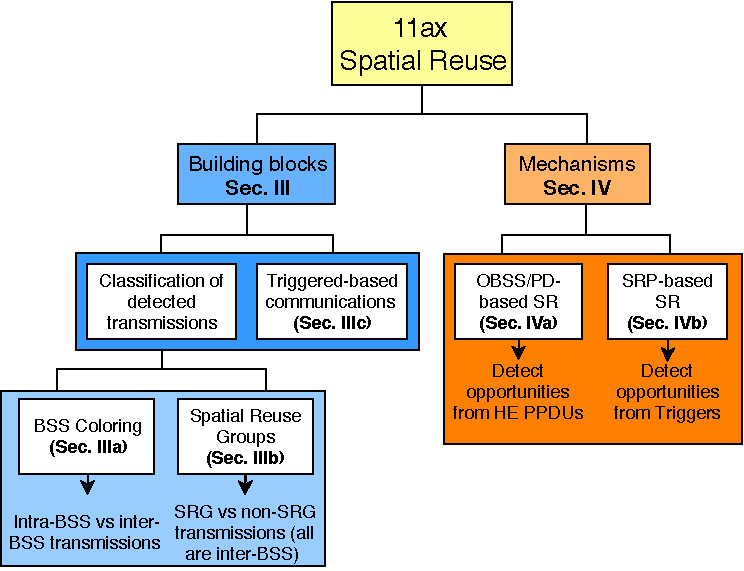
\includegraphics[width=\columnwidth]{sr_summary}
		\caption{Summary of the 11ax SR operation.}
		\label{fig:sr_summary}
	\end{figure}
	
	In order to illustrate the potential SR enhancement in an OBSS, let us focus on Fig.~\ref{fig:spatial_reuse_11ax}. Unlike typical coverage representations in wireless networks, throughout this paper, we consider the carrier sense area of each device (instead of the generated interference). For that, our representation assumes that the transmission power used by any device is fixed and that all the WLANs are in the same channel. Accordingly, the dashed circles in Fig.~\ref{fig:spatial_reuse_11ax} indicate the transmitters that can be detected by the node of interest. In our example, both Access Points (APs) can simultaneously transmit to their corresponding stations (STAs), provided that they use the enhanced combination of CST and transmission power (bold line). In contrast, parallel transmissions are not possible when using the default configuration.
	\begin{figure}[ht!]
		\centering
		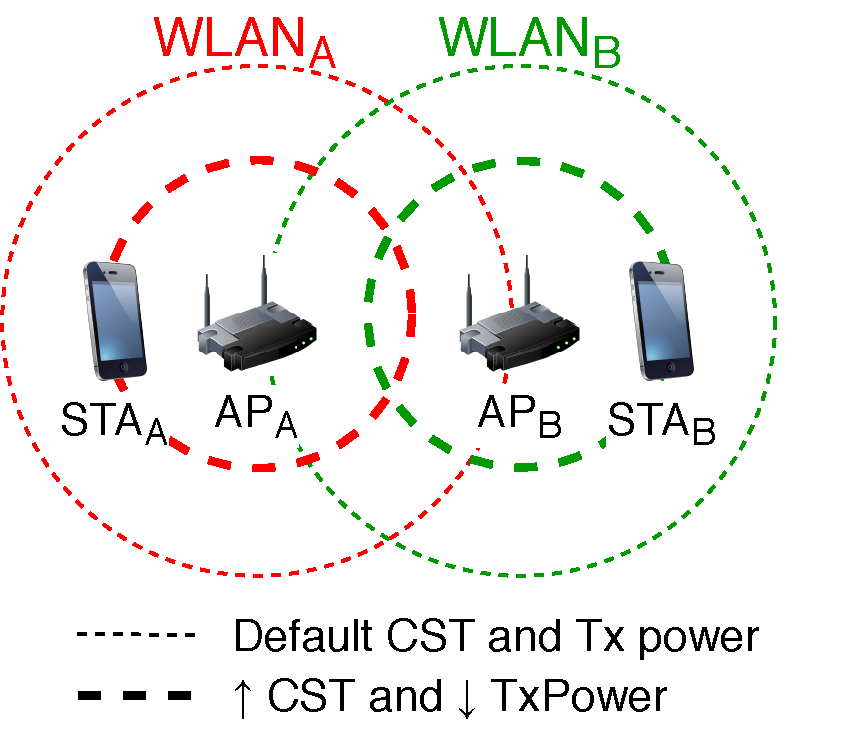
\includegraphics[width=0.33\textwidth]{fig_1.pdf}
		\caption{SR enhancement through CST adjustment and TPC. The carrier sensing area of each transmitter is graphically represented by the dashed lines.}
		\label{fig:spatial_reuse_11ax}
	\end{figure}
	
	In spite of the apparent benefits of the SR operation, its actual potential is still unknown. In some situations, dynamic sensitivity and transmission power adjustment have been shown to significantly increase the network performance and to contribute to reducing the effects of the well-known hidden and exposed terminal problems \cite{zhou2005balancing}. However, in some other cases, these problems may be exacerbated as well \cite{wilhelmi2019potential}. Indeed, modifying either the CST or the transmit power can worsen the hidden/exposed terminal problems by generating flow starvation and asymmetries.
	
	Fig. \ref{fig:policies_sr} shows in an intuitive manner the effect of increasing and decreasing both the transmission power and the sensitivity in an OBSS. For instance, an increase in the sensitivity of a device may contribute to accessing the channel more often since the listening area is reduced. However, that can also lead to a higher number of collisions by hidden-node.
	\begin{figure}[ht!]
		\centering
		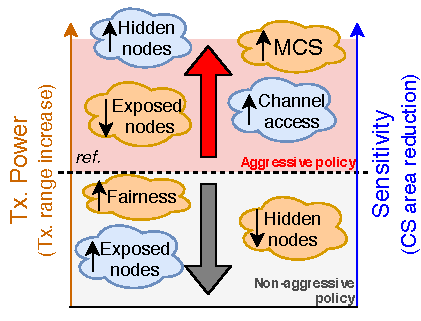
\includegraphics[width=0.8\columnwidth]{policies_sr}
		\caption{Effects of different policies with regards to sensitivity adjustment and transmission power control.}
		\label{fig:policies_sr}
	\end{figure}
	
	Therefore, dealing with the spatial dimension may lead to severe implications and generate complex inter-WLAN interactions that are hard to predict beforehand. Indeed, the SR operation is one of the least studied features in next-generation WLANs. In fact, only a few works have delved into the 11ax SR operation and have assessed its potential. 
	
	Firstly, the authors in \cite{mori2014performance} evaluated the benefits of using dynamic sensitivity thresholds for inter-BSS transmissions, given a fixed transmit power. Secondly, the work in \cite{qu2018survey} exhaustively surveyed the 11ax amendment, thus providing an overview of the first drafted SR operation. Moreover, it provided some results on applying SR in both indoor and outdoor scenarios. For the former, a high potential was shown with regards to throughput maximization. Similarly, the authors in \cite{shen2018research} introduced the contents of the 11ax SR as they are described in the amendment. In addition, they provided a performance evaluation based on the adjustment of the inter-BSS sensitivity threshold. Their results showed significant gains when applying SR, especially for dense scenarios. 

	Unlike in \cite{mori2014performance, qu2018survey, shen2018research}, in this paper we delve into the 11ax SR operation in more detail since we consider the two different SR operations included in the 11ax amendment. In addition, our analysis of the 11ax SR is not limited to the technical information included in the amendment. Instead, we accompany our descriptions with illustrative use cases, thus bringing a new perspective that allows devising the real utility behind the operation. We thus go beyond the definition of the specification, shedding light on its purpose, benefits, and challenges.
	
	% Contributions
	Our aim in this paper not only lies in providing a comprehensive tool for researchers interested in the topic, but to analyze the potential of the SR operation in future WLANs. Moreover, we focus on the potential gaps in the standard to be filled by the research community. The main contributions of this paper lie in the description, analysis, and evaluation of the 11ax SR operation. In particular:
	\begin{enumerate}
		\item We provide a gentle, exhaustive, and comprehensive overview of the SR operation included in the 11ax amendment.
		\item We model the SR operation and capture the interactions between WLANs through an analytical model. The results of this model are verified with an 11ax-based simulator \cite{barrachina2019komondor}.
		\item We explore the potential of the SR operation in improving network efficiency in dense WLANs through simulations. %We expect that our results can be later used for future developments in other well-known simulation tools \st{such as ns-3 \cite{riley2010ns}~\textcolor{red}{IMO the ns-3 webpage should also be used}}.
		\item We delve into the gaps and gray areas existing in the current 11ax SR operation and elaborate on future research directions in the field. %An important remark is that the IEEE 802.11ax does not include the exact procedures to concisely achieve SR, which opens the door to the research community to contribute towards SR enhancement in IEEE 802.11 WLANs. Instead, it establishes a set of limitations regarding the possible transmission power and sensitivity values. Besides, it establishes the communication procedures and the data formats to be used by HE-stations (HE-STAs) to implement the SR operation. 
	\end{enumerate}
	
	% Document structure
	The remainder of this document is structured as follows. Section \ref{section:previous_work_sr} surveys the related work on SR in WLANs. The specifications and procedures that enable the 11ax SR operation are described in Section \ref{section:enablers_sr_11ax} and Section \ref{section:operation_sr_11ax} details the operation itself. Section~\ref{section:analytical_model} presents an analysis-based study of the SR operation in simple scenarios, whilst Section~\ref{section:performance_evaluation} studies the SR operation in more complex/dense deployments through simulations. Section \ref{section:ways_forwad} identifies the gaps and research opportunities found within the 11ax SR operation and explores potential ways forward. Finally, Section~\ref{section:conclusions} provides some concluding remarks.
	
	% ----------------------------------
	% -
	% 	-- Previous Work on SR --
	% -
	% ----------------------------------
	\section{Spatial Reuse techniques in IEEE 802.11 WLANs}%\section{Related Work on Spatial Reuse in IEEE 802.11 WLANs}
	\label{section:previous_work_sr}
	
	\begin{figure*}[ht!]
		\centering
		\subfigure[Scenario]{\label{fig:11ax_bss_coloring_a}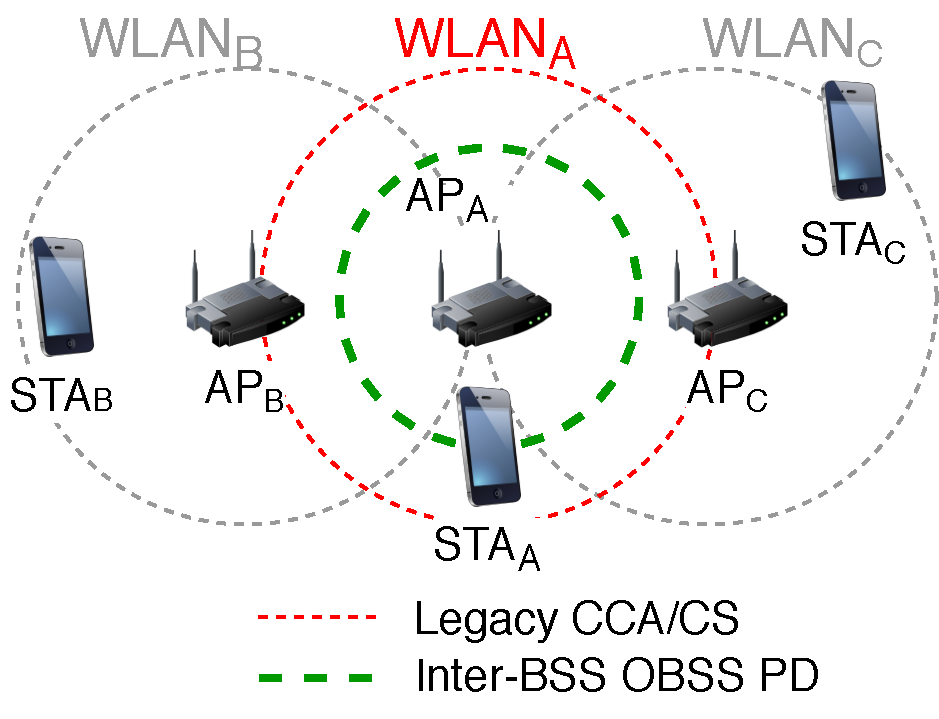
\includegraphics[width=0.65\columnwidth]{fig_2a}}
		\hspace{1cm}
		\subfigure[Packets exchange]{\label{fig:11ax_bss_coloring_b}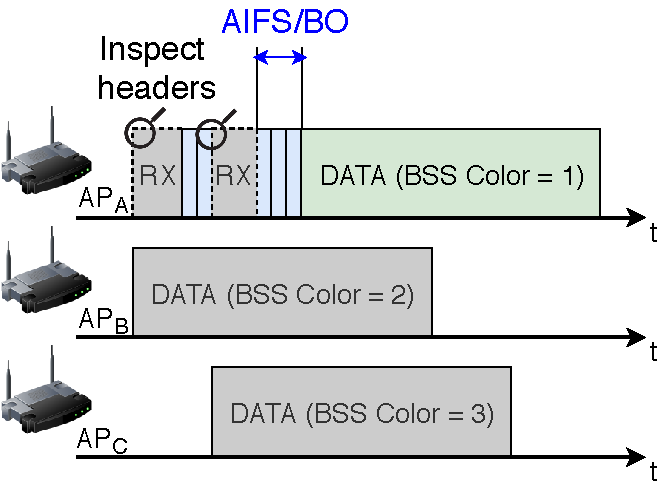
\includegraphics[width=0.7\columnwidth]{fig_4b}}
		\caption{Channel access rules based on BSS coloring. In (b), the propagation delay is considered to be negligible.}
	\end{figure*}
	
	When it comes to IEEE 802.11 WLANs, we find few works related to the 11ax SR operation. Nonetheless, the problem of dynamic sensitivity and transmission power adjustment has been addressed in multiple ways. On the one hand, we find centralized solutions such as the ones proposed in \cite{li2011achieving, jamil2016novel, nakahira2014centralized}, where the SR operation is controlled and mandated from the APs. Among these, we highlight \cite{jamil2016novel}, which uses a method based on Neural Networks (NN) to compute the best combination of sensitivity and transmit power to be used by all the WLANs in a given scenario. Nonetheless, centralized approaches require coordination and extra overhead, which is usually impractical.
	
	On the other hand, SR has been addressed through a decentralized perspective in \cite{chevillat2005dynamic, tang2011improving, chau2017effective, wilhelmi2019collaborative, wilhelmi2019potential}. Most of the decentralized strategies rely on collecting feedback on several performance metrics (e.g., sensed interference, packets lost, etc.). While works such as \cite{chevillat2005dynamic, tang2011improving, chau2017effective} propose adaptive mechanisms to adjust the CST and/or the transmission power, some others like \cite{wilhelmi2019collaborative, wilhelmi2019potential} provide probabilistic approaches based on Reinforcement Learning (RL) for finding the best possible configuration.
	
	Regarding the 11ax amendment itself, the Dynamic Sensitivity Control (DSC) scheme was proposed to be included in the standard as the official SR solution, but it was never incorporated. The performance of DSC was evaluated in \cite{afaqui2015evaluation, afaqui2016dynamic, kulkarni2015taming}. Furthermore, the authors in \cite{selinis2016evaluation, selinis2017exploiting} combined DSC with BSS color schemes to devise further improvements in WLANs.
	
	The current 11ax SR operation has nonetheless been studied to a lower extent. Based on the OBSS/PD-based SR operation, the work in \cite{selinis2018control} proposed a new mechanism to adjust the OBSS/PD threshold.\footnote{The OBSS/PD threshold refers to the sensitivity to be used for detected inter-WLAN transmissions.} This mechanism, so-called Control OBSS/PD Sensitivity Threshold (COST), differs from DSC in terms of the information available in 11ax nodes. In this case, nodes are supposed to be aware of any change in the OBSS. 
	
	Unlike previous works, we focus on the IEEE 802.11ax SR operation defined in Draft v4.0 and delve into its potential through analytical modeling and a simulation tool. Moreover, we identify potential gaps and research opportunities with regard to the amendment.

	% ----------------------------------
	% -
	% 	-- IEEE 802.11ax Preliminaries --
	% -
	% ----------------------------------
	\section{IEEE 802.11ax Spatial Reuse Operation: Building Blocks}
	\label{section:enablers_sr_11ax}
	In order to understand the 11ax SR operation in detail we must first introduce the concepts and features that are the enablers of the operation itself. In particular, the 11ax SR operation can be understood through the \textbf{BSS coloring} and \textbf{Spatial Reuse Groups (SRG)}. In addition, it is important to know the basics on \textbf{Triggered-based (TB) transmissions}, which are the foundations upon which the SRP-based SR operation is built.
	
	%% BSS COLORING
	\subsection{BSS coloring}	
	\label{section:bss_coloring}	
	BSS coloring is a key enabler of the 11ax SR operation, whereby HE nodes can rapidly identify the source of a given transmission. Accordingly, WLANs can effectively determine whether the channel is occupied by a device of the same WLAN (intra-BSS transmission, same color) or from another one (inter-BSS transmission, different color). The BSS color, which is determined by the AP and is included in the preambles of Wi-Fi frames,\footnote{The \texttt{BSS color} field is included in the Physical Layer Convergence Procedure (PLCP) header. See Appendix \ref{section:frames} for further details.} is a value in the range of 1 to 63. It remains static until the AP considers to change it. In case of noticing a BSS color overlap (i.e., two different WLANs use the same color), a new color may be chosen by the affected APs. 
	
	The method for selecting a new color is out of the scope of the 11ax amendment, but the advertising operation is actually defined. An HE AP may announce a new BSS color via the \texttt{BSS Color Change Announcement} element, which is carried in Beacon, Probe Response and (Re)Association Response frames. 
	
	% Intra-BSS and Inter-BSS frames
	\subsubsection{BSS color-based channel access rules}
	\label{section:bss_color_channel_access}
	
	\begin{figure*}[ht!]
		\centering
		\subfigure[Scenario]{\label{fig:fig_5_a}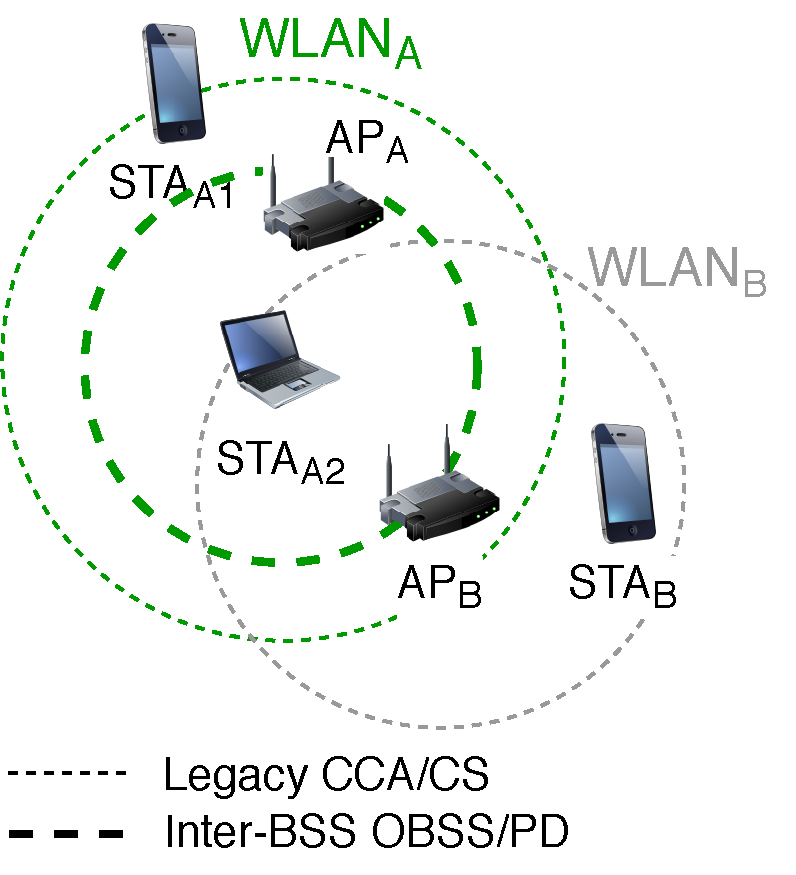
\includegraphics[width=0.65\columnwidth]{fig_5_a}}
		\hspace{1cm}
		\subfigure[Packets exchange]{\label{fig:fig_5_b}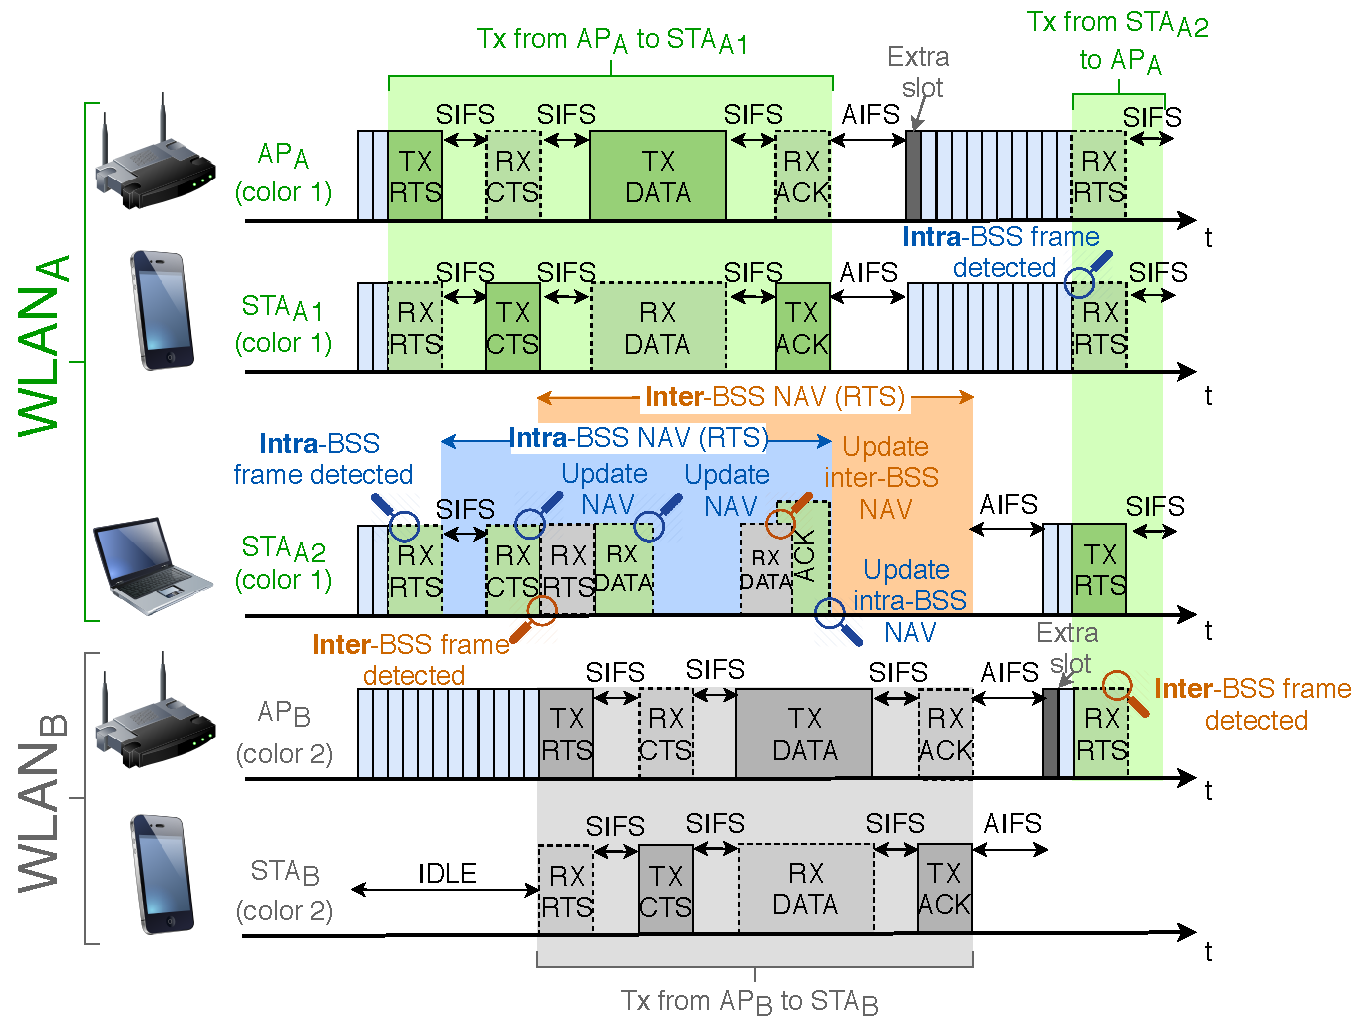
\includegraphics[width=1.2\columnwidth]{fig_5_b}}
		\caption{Two NAVs operation in an OBSS.}
		\label{fig:two_navs}
	\end{figure*}
	
	When detecting a transmission, an HE node can distinguish between intra and inter-BSS frames by rapidly inspecting the \texttt{BSS color} field that is carried in every HE PLCP Protocol Data Unit (PPDU).\footnote{In case that the \texttt{BSS color} is not announced, frames can be classified according to the \texttt{GROUP\_ID} and \texttt{PARTIAL\_AID} in VHT PPDUs, or the MAC address in the MAC header of legacy frames (i.e., predecessor amendments of the IEEE 802.11ac).} In particular, the default PD threshold (i.e., -82 dBm) is used for intra-BSS frames. So, from now onwards, we will refer to the default PD threshold simply as Clear Channel Assessment / Carrier Sense (CCA/CS). On the contrary, when inter-BSS frames are detected, more aggressive PD thresholds can be applied to increase the number of parallel transmissions. Those PD thresholds are termed \textbf{non-SRG OBSS/PD} and \textbf{SRG OBSS/PD}. The SRG OBSS/PD is used when spatial reuse groups are allowed, which is discussed in detail in Section \ref{section:srg}.
	
	Now, in order to illustrate how BSS coloring can help at enhancing SR, let us consider the scenario shown in Fig. \ref{fig:11ax_bss_coloring_a}. In this scenario, $\text{AP}_{A}$ suffers from flow starvation if the default CCA/CS value is used, which entails being in the range of both $\text{AP}_B$ and $\text{AP}_C$. Note that simultaneous transmissions can be held in both $\text{WLAN}_B$ and $\text{WLAN}_C$ because their devices are not in the range of each other. Therefore, they monopolize the channel and generate starvation to $\text{WLAN}_A$. Nevertheless, using a higher CST value for inter-BSS frames allows $\text{AP}_{A}$ to ignore transmissions from $\text{AP}_B$ and $\text{AP}_C$. 
	
	As shown in Fig. \ref{fig:11ax_bss_coloring_b}, $\text{AP}_A$ first identifies the source of a detected transmission by inspecting its headers. Then, it uses a less conservative CST for inter-BSS communications, which in this case is referred to as the non-SRG OBSS/PD. This CST value allows $\text{AP}_A$ to continue the backoff procedure and eventually transmit, increasing spectral efficiency.
	
	% Two NAVs
	\subsubsection{Two NAVs}
	\label{section:two_navs}
	The SR operation entails significant changes on the virtual carrier sensing procedure, which roughly consist in maintaining two different Network Allocation Vectors (NAVs), i.e., \emph{intra-BSS NAV} and \emph{inter-BSS NAV} for intra and inter-BSS frames, respectively. According to that, a given transmitter can decrease its backoff counter only if both NAV timers are set to zero. Otherwise, it must remain idle for at least the duration of the ongoing transmission(s),\footnote{The duration used for setting the NAV is indicated in the Duration field of a Physical layer Service Data Unit (PSDU).} which had previously activated the virtual carrier sensing. 
	
	To showcase the utilization of two NAVs within the SR operation, we consider the scenario shown in Fig. \ref{fig:fig_5_a}, where packets are exchanged as illustrated in Fig. \ref{fig:fig_5_b}. In this scenario, $\text{WLAN}_A$ and $\text{WLAN}_B$ are considered to be within the same sensitivity area, provided that they both use the same CCA/CS value. In opposite, both WLANs can ignore each others' transmissions in case of applying SR based on the BSS Color.
	
	By following the Distributed Coordination Function (DCF) operation, $\text{AP}_A$ sends a Request-to-Send (RTS) frame to $\text{STA}_\text{A1}$, in order to start a downlink transmission to that node. Then, $\text{STA}_\text{A2}$ decodes the RTS frame and realizes that it was sent by a device belonging to the same WLAN (the BSS color field matches with its own). In other words, the RTS is classified as an intra-BSS frame. As a result, $\text{STA}_\text{A2}$ uses the default CCA/CS threshold and enters into a virtual carrier sense state by using the intra-BSS NAV. Note that a legacy device simply attempts to decode the RTS frame and decide whether the channel is occupied or not according to the legacy CCA/CS threshold. It is also worth mentioning that the NAV timer is updated in $\text{STA}_\text{A2}$ when $\text{STA}_\text{A1}$ sends the Clear-to-Send (CTS) frame to $\text{AP}_A$, because they are in the sensing range. 
	
	In parallel to those intra-BSS interactions, $\text{AP}_B$ starts its own downlink transmission to $\text{STA}_B$. The RTS that initiates such a transmission is also listened by $\text{STA}_\text{A2}$, which sets the inter-BSS NAV accordingly. In this occasion, the acknowledgments sent by $\text{STA}_B$ are ignored by $\text{STA}_\text{A2}$ due to the OBSS/PD threshold employed for inter-BSS transmissions. However, it has no impact on the modification of the inter-BSS NAV, which is properly set by the frames transmitted by $\text{AP}_B$. Finally, once both timers are over, $\text{STA}_\text{A2}$ can perform an uplink transmission, provided that it gains access to the channel.
	
	The utility behind maintaining two NAVs becomes evident for dense deployments. On the one hand, the intra-BSS NAV allows protecting STAs from intra-BSS transmissions, thus reducing the effect of certain anomalies such as the hidden-terminal problem. On the other hand, as a novelty, the inter-BSS NAV allows mitigating OBSS interference, which contributes to increasing the number of parallel transmissions. 
	
	%%% SR groups
	\subsection{Spatial Reuse Groups}
	\label{section:srg}
	To further enhance network efficiency, the 11ax provides a mechanism that allows differentiating between two types of inter-BSS frames; that is to say, belonging or not to the same SRG. These groups can be formed by WLANs to achieve a more sophisticated SR operation. For instance, more aggressive channel access policies can be used for transmissions within the same SRG, in case that higher levels of interference could be supported by the nodes of the same SRG. Or it could be the other way around. A conservative policy can be employed for the sake of minimizing collisions by hidden nodes. 
	
	Despite that the formation of SRGs is out of the scope of the amendment, differentiating between two OBSS/PD thresholds can be useful for capturing more subtle inter-WLAN interactions. Note, as well, that SRGs could be formed online to address some issues detected by an entity controlling a set of APs (e.g., belonging to the same operator).
	
	Fig. \ref{fig:fig_4} shows a scenario in which the formation of SRGs makes sense. In this case, the channel utilization can be enhanced through the non-SRG OBSS/PD (light dashed lines). However, if doing so homogeneously, $\text{STA}_C$ is expected to suffer packet losses. In particular, $\text{STA}_C$ cannot properly decode the information sent by $\text{AP}_C$ when $\text{AP}_A$ also occupies the channel. Nevertheless, $\text{WLAN}_A$ and $\text{WLAN}_C$ can form a group and employ a more conservative OBSS/PD threshold (i.e., SRG OBSS/PD), so that parallel transmissions between these two WLANs are not possible. Besides, the non-SRG OBSS/PD threshold (which is more aggressive) can be still employed for transmissions held by any pair of WLANs involving $\text{WLAN}_B$, thus increasing network efficiency. As shown, not only the formation of SRGs is a complex task, but also the definition of both non-SRG and SRG OBSS/PD thresholds.
	
	\begin{figure}[ht!]
		\centering
		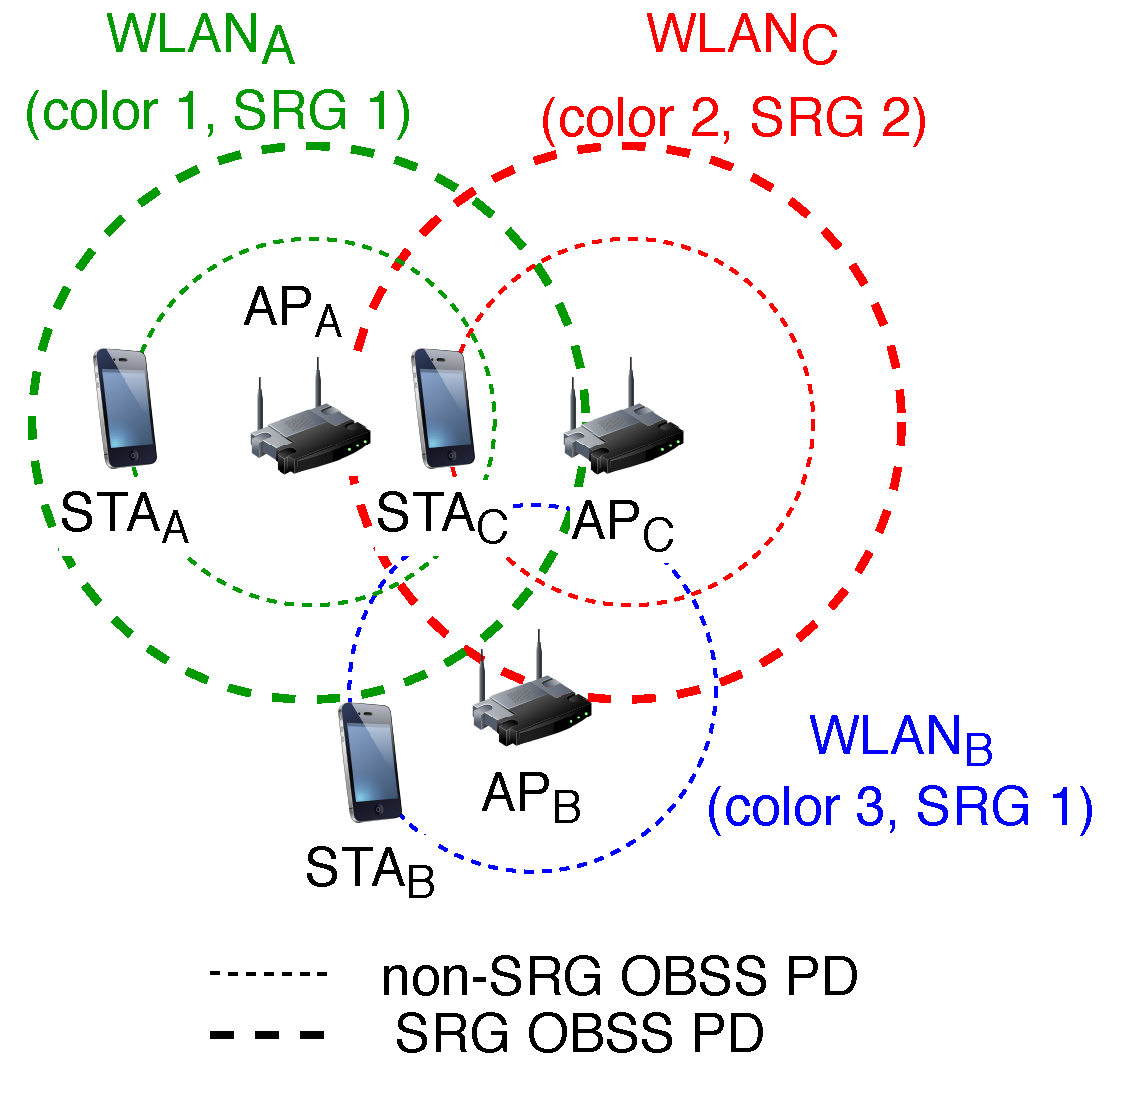
\epsfig{file=fig_4.pdf, width=6cm}
		\caption{Spatial Reuse Groups in an OBSS.}
		\label{fig:fig_4}
	\end{figure}
	
	In order to apply the SR operation based on SRGs, the involved HE nodes must have indicated support to this feature. With regards to HE STAs, they enable the SRG operation upon the reception of an activating \texttt{Spatial Reuse Parameter Set} element (further described in Appendix \ref{section:srps}) from their AP. Then, for the following detected PPDUs, both HE APs and STAs may differentiate between SRG and non-SRG PPDUs. Note that 11ax devices can also identify the source of non-HE transmissions. Therefore, not only HE devices are supported but also legacy devices. The way of classifying frames according to the SRG is backward compatible with previous IEEE 802.11 amendments. Technically speaking, SRG identification is done as follows:
	\begin{itemize}
		\item In case of detecting an HE PPDU, the HE STA inspects the \texttt{BSS color} and checks if it belongs to the same SRG. Such information is kept on the \texttt{SRG BSS Color Bitmap} of the \texttt{Spatial Reuse Parameter Set}, which stores the different BSS colors that belong to the same SRG. The AP of a given WLAN is responsible for maintaining the SRG BSS Color Bitmap up to date, and to inform STAs in case of noticing any change.
		\item When it comes to VHT PPDUs, inter-BSS transmissions are considered to belong to the same SRG if the \texttt{GROUP\_ID} parameter (included in the \texttt{RXVECTOR}\footnote{The RXVECTOR constitutes a set of parameters that the PHY layer delivers to the MAC on receiving a PPDU.}) has a value of 0, and the bit in the \texttt{SRG Partial BSSID Bitmap} field corresponding to the numerical value of \texttt{PARTIAL\_AID}\footnote{The \texttt{PARTIAL\_AID} is an identifier which, similarly to the BSS color, is used by IEEE 802.11ac WLANs to quickly identify the source of a transmission.} (also included in the \texttt{RXVECTOR}) is set to 1. 
		\item Finally, regarding other types of PPDU, they are classified as SRG PPDUs if the BSSID information from a MAC Protocol Data Unit (MPDU) of the PPDU is correctly received and the bit in the \texttt{SRG Partial BSSID Bitmap} field corresponding to the numerical value of BSSID is 1.
	\end{itemize}
	
	% SRG and non-SRG frames
	\subsubsection{SRG-based Channel Access Rules}
	\label{section:srg_channel_access}
	\begin{figure}[ht!]
		\centering
		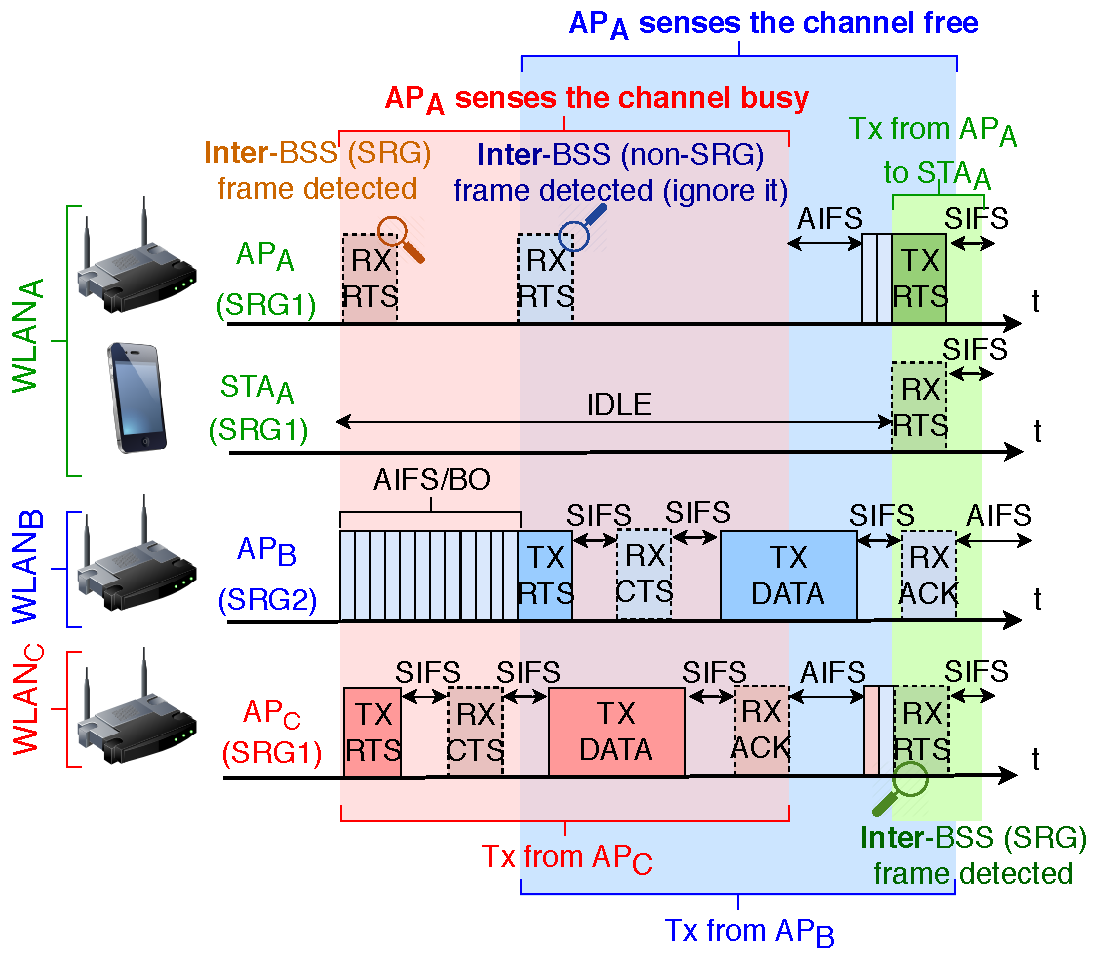
\includegraphics[width=\columnwidth]{fig_7}
		\caption{Packets exchange based on SRG channel access rules.}
		\label{fig:srg_channel_access}
	\end{figure}
	
	Differentiating between SRGs may provide higher SR enhancements than considering only one type of inter-BSS frame. Despite the specific utilization of SRGs is also out of the scope of the 11ax amendment, we can devise several situations where its application can be useful. As previously pointed out, one possibility is to establish groups for those WLANs whose transmissions need to be protected. In other words, an HE STA detecting an SRG frame can implement a more conservative channel access policy. Conversely, a more aggressive policy can be applied for non-SRG PPDUs, thus increasing the number of parallel transmissions. 
	
	In order to illustrate the SRG-based channel access rules, let us retake the scenario shown in Fig. \ref{fig:fig_4}, where three overlapping WLANs share the medium. While $\text{WLAN}_A$ and $\text{WLAN}_B$ belong to SRG 1, $\text{WLAN}_C$ belongs to SRG 2. Accordingly, different power detection mechanisms are applied by $\text{WLAN}_A$ when detecting inter-BSS frames belonging to groups 1 or 2 (note that all the WLANs use different BSS colors). 
	
	As shown in Fig. \ref{fig:srg_channel_access}, transmissions from $\text{WLAN}_C$ (in blue) provoke that $\text{AP}_A$ senses the channel busy. In contrast, packets detected from $\text{WLAN}_B$ (in red) are ignored by $\text{AP}_A$ after PHY headers are inspected. In this example, a less restrictive OBSS/PD is applied for transmissions within the same SRG than for non-SRG ones. The fact is that $\text{STA}_B$ is sufficiently far away from $\text{AP}_A$. Therefore, simultaneous transmissions between $\text{WLAN}_A$ and $\text{WLAN}_B$ are completely feasible. The opposite occurs for $\text{WLAN}_A$-$\text{WLAN}_C$ interactions. In this case, collisions may occur at STA$_C$ if simultaneous transmissions are held, thus requiring additional protection.
	
	%% TB communications
	\subsection{Triggered-based communications}
	\label{section:tb_communication}
	As previously pointed out, one of the 11ax SR operations relies on TB transmissions \cite{bellalta2019ap}. Roughly, in a TB communication, an AP schedules UL transmissions from one or more STAs. To that purpose, a Trigger Frame (TF) is sent by a given AP to indicate the group of users that are allowed to transmit during the current Transmission Opportunity (TXOP), along with other relevant information. Fig. \ref{fig:TB_transmission_example} illustrates an example of a TB transmission. After gaining access to the channel, the AP first sends a TF packet, which is received by HE STAs. Upon successful reception of the TF, STAs start their TB UL transmissions simultaneously, which can be enabled by using multiple antenna technologies (i.e., MU-MIMO) or different OFDMA subcarriers. Once all the transmissions are finished, the AP acknowledges all the packets with a multi-station block ACK (MACK).
	\begin{figure}[ht!]
		\centering
		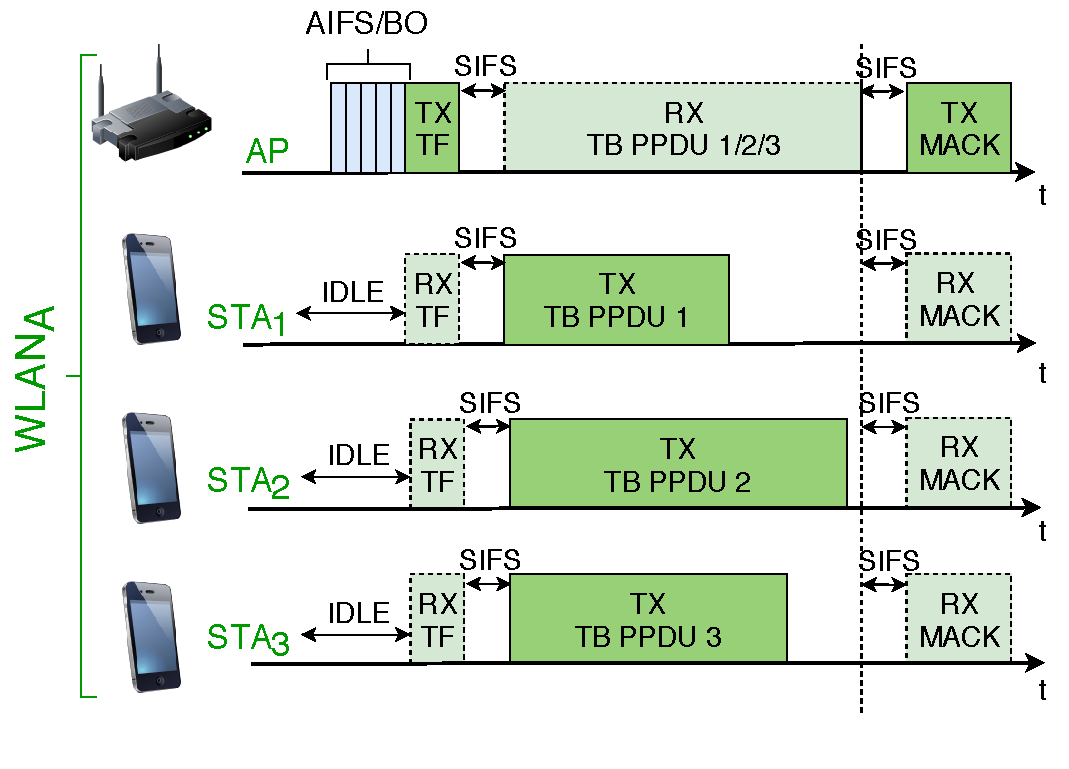
\includegraphics[width=\columnwidth]{fig_8}
		\caption{TB UL transmission held in a WLAN.}
		\label{fig:TB_transmission_example}
	\end{figure}
	
	\begin{figure*}[ht!]
		\centering
		\begin{minipage}{\columnwidth}
			\centering
			\vbox{%
			\vfill	\subfigure[Scenario]{\label{fig:fig_9a}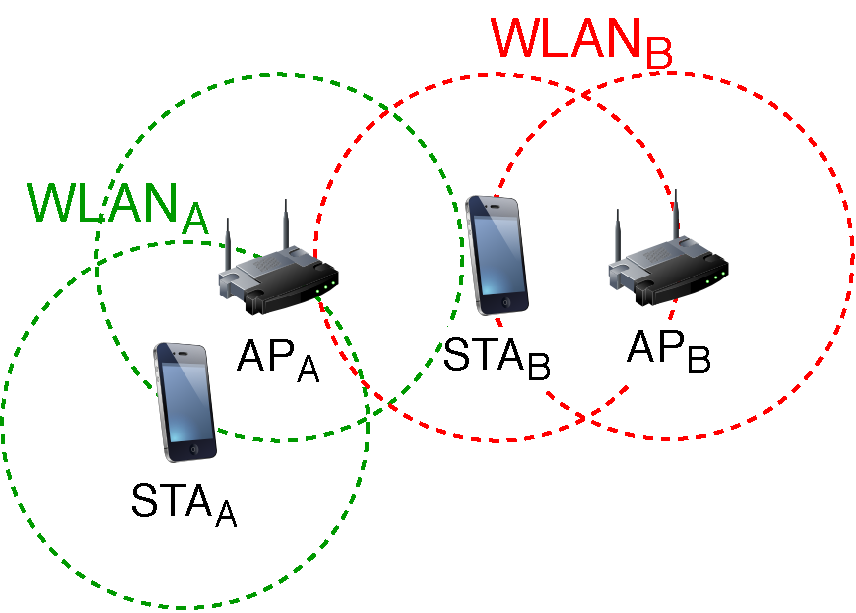
\includegraphics[width=0.65\columnwidth]{fig_9a}}
			\vfill}
		\end{minipage}
		\begin{minipage}{\columnwidth}
			\centering
			\vbox{%
			\vfill
			\subfigure[Packets exchange]{\label{fig:fig_9b}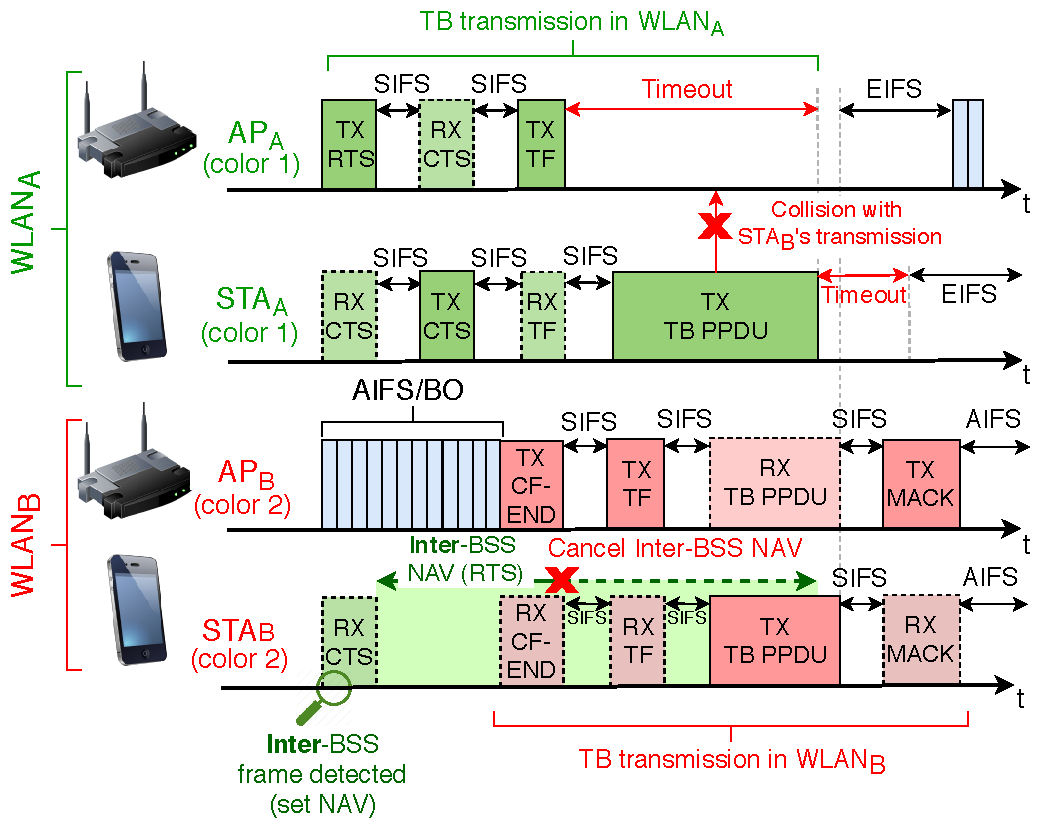
\includegraphics[width=\columnwidth]{fig_9b}}
			\vfill}
		\end{minipage}
		\caption{NAV cancellation anomaly in TB UL transmissions. $\text{AP}_{B}$ is not in range of neither $\text{AP}_{A}$ nor $\text{STA}_{A}$, so it cancels the NAV in $\text{STA}_{B}$ through a CF-End frame before starting a TB transmission. As a result, a collision occurs at $\text{WLAN}_{A}$.}
		\label{fig:two_navs_issues}
	\end{figure*}
	
	In particular, the SR operation takes advantage of TB communications for detecting what is called SRP opportunities. By inspecting an inter-BSS TF packet, an HE STA implementing SRP-based SR can determine the maximum allowed interference by the inter-BSS AP scheduling the transmission. As a result, it can transmit during the TXOP at a regulated transmission power. Further details on this are provided in Section \ref{section:srp_based}.
	
	Finally, it is worth mentioning that, before scheduling a UL transmission, APs can cancel the virtual carrier sensing of their STAs by sending a Contention Free End (CF-End) control frame. This is done to reduce the idle periods provoked by inter-BSS transmissions, thus enhancing network efficiency. Nonetheless, some performance anomalies can occur. In particular, canceling the inter-BSS NAV of a STA may lead to collisions. To illustrate such an anomaly, let us refer to Fig.~\ref{fig:two_navs_issues}, where $\text{STA}_{B}$ sets an inter-BSS NAV when $\text{AP}_{A}$ schedules an UL transmission from $\text{STA}_{A}$. Since $\text{AP}_{B}$ is unaware of that transmission, it may send a CF-End frame to $\text{STA}_{B}$ to cancel the inter-BSS NAV before initiating another TB UL communication. As a consequence, a collision occurs in $\text{AP}_{A}$.
	
	% ----------------------------------
	% -
	% 	-- IEEE 802.11ax --
	% -
	% ----------------------------------
	
	\section{IEEE 802.11ax Spatial Reuse Operation}
	\label{section:operation_sr_11ax}
	The IEEE 802.11ax SR operation is divided into two different mechanisms: \emph{i)} \textbf{OBSS/PD-based SR} and \emph{ii)} \textbf{SRP-based SR}. So far, we have described the elements that enable both operations, thus providing insights on the potential of applying SR. In this Section, we show the technical details of the IEEE 802.11ax SR operation, thus embodying the concepts that have been previously introduced in Section \ref{section:enablers_sr_11ax}.
	
	%% OBSS_PD-BASED SR
	\subsection{OBSS/PD-based Spatial Reuse}
	\label{section:obss_pd_based}
	The OBSS/PD-based SR operation is based on the adjustment of the CST and the transmission power after detecting an inter-BSS frame. By knowing the source of an ongoing transmission, an HE STA may employ different CST values, thus improving spectral efficiency. This operation aims to increase the channel utilization when other WLANs are transmitting. In particular, when a PPDU reception starts at any HE node, the MAC layer receives a notification from the PHY. At that moment, the node inspects the packet and, among several operations, it determines whether the PPDU is an intra-BSS or an inter-BSS frame. The latter may be subdivided into SRG or non-SRG frames, provided that SRGs are enabled.
	
	% General constraints
	\subsubsection{General constraints}
	As a general rule, the OBSS/PD threshold that is used for detected inter-BSS frames cannot exceed a certain value. This upper bound is illustrated in Fig. \ref{fig:fig_7}, and is defined as follows:
	\begin{align}\nonumber \text{OBSS/PD} \leq & \max\Big(\text{OBSS/PD}_{\min}, \min\big(\text{OBSS/PD}_{\max},\\ & \text{OBSS/PD}_{\min} + (\text{TX\_PWR}_{\text{ref}}-\text{TX\_PWR})\big)\Big), \nonumber \end{align}
	where $\text{OBSS/PD}_{\min}$ and $\text{OBSS/PD}_{\max}$ are set to $-82$ dBm and $-62$ dBm, respectively, the reference power $\text{TX\_PWR}_{\text{ref}}$ is set to 21 or 25 dBm, according to the
	capabilities of the device,\footnote{The $\text{TX\_PWR}_{\text{ref}}$ is set to 21 dBm at HE nodes which \texttt{Highest NSS Supported M1} field is equal or less than 1. Otherwise, the  $\text{TX\_PWR}_{\text{ref}}$ is set to 25 dBm. The \texttt{Highest NSS Supported M1} subfield is part of the \texttt{Tx Rx HE MCS Support} field of the \texttt{HE Capabilities element}.} and $\text{TX\_PWR}$ is the transmission power at the antenna connector in dBm of the HE node that identifies the SR-based opportunity.
	\begin{figure}[ht!]
		\centering
		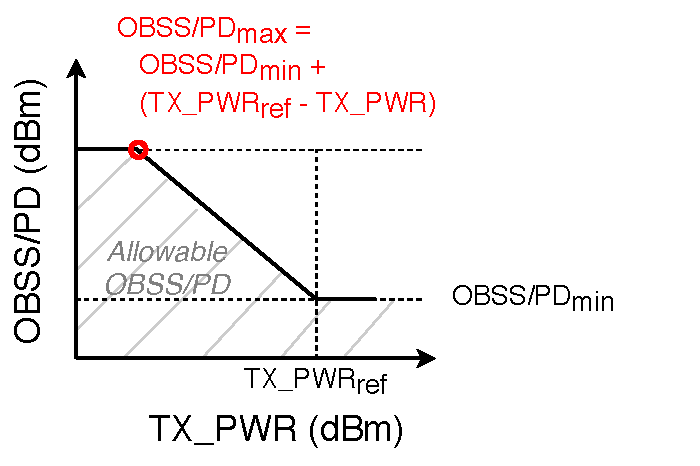
\includegraphics[width=0.8\columnwidth]{fig_10}
		\caption{Graphical representation of the adjustment rules for OBSS/PD and transmission power \cite{tgax2019draft}.}
		\label{fig:fig_7}
	\end{figure}
	
	Note that the $\text{OBSS/PD}$ is defined for 20 MHz PPDUs received on the primary channel, but, in general, this value depends on the bandwidth used. In particular, the $\text{OBSS/PD}$ increases 3 dB each time the channel width is doubled, as shown in Table \ref{tbl:sensitivity_channel_width}.
	\begin{table}[ht!]
		\centering
		\resizebox{0.9\columnwidth}{!}{\begin{tabular}{|c|l|}
			\hline
			\textbf{Channel width} & \multicolumn{1}{c|}{\textbf{$\text{OBSS/PD}$}} \\ \hline
			40 MHz & $\text{OBSS/PD}_{20 \text{MHz}}$ + 3 dB \\ \hline
			80 MHz & $\text{OBSS/PD}_{20 \text{MHz}}$ + 6 dB \\ \hline
			160 MHz or 80+80 MHz   & $\text{OBSS/PD}_{20 \text{MHz}}$ + 9 dB \\ \hline
		\end{tabular}}
		\caption{Effect of the channel width on the OBSS/PD threshold.}
		\label{tbl:sensitivity_channel_width}
	\end{table}	
	
	% SRG constraints
	\subsubsection{SRG-based constraints}	
	In addition to the general rules for the OBSS/PD, further constraints apply when using SRGs. In particular, an AP can define certain tolerance margins for setting both the SRG and the non-SRG OBSS/PD (see Tables \ref{tbl:non-srg} and \ref{tbl:srg}). Those margins are named minimum and maximum OBSS/PD offset, respectively, and must verify:
	\begin{itemize}
		\item -82 dBm $\leq$ -82 dBm + SRG OBSS/PD Min Offset dBm $\leq$ -62 dBm 
		\item SRG OBSS/PD Min Offset $\leq$ SRG OBSS/PD Max Offset
		\item SRG OBSS/PD Max Offset + -82 dBm $\leq$ -62 dBm 
		\item Non-SRG OBSS/PD Max Offset + -82 dBm $\leq$  -62 dBm
	\end{itemize}
	
	\begin{table}[ht!]
		\centering
		\resizebox{\columnwidth}{!}{	\begin{tabular}{|c|c|c|c|}
			\hline	\textbf{\begin{tabular}[c]{@{}c@{}}OBSS/PD SR \\ Disallowed\end{tabular}} & \textbf{\begin{tabular}[c]{@{}c@{}}Non-SRG \\Offset\end{tabular}} & \textbf{\begin{tabular}[c]{@{}c@{}}Non-SRG \\OBSS/PD Min\end{tabular}} & \textbf{\begin{tabular}[c]{@{}c@{}}Non-SRG \\OBSS/PD Max\end{tabular}} \\ \hline	\begin{tabular}[c]{@{}c@{}}Unspecified\end{tabular} & \begin{tabular}[c]{@{}c@{}}Unspecified\end{tabular} & -82 & -62 \\ \hline 
			0 & 0 & -82 & -62 \\ \hline
			0 & 1 & -82 & \begin{tabular}[c]{@{}c@{}}-82 + Non-SRG \\OBSS/PD Max off.\end{tabular} \\ \hline
			1 & Don't care & -82 & -82 \\ \hline
		\end{tabular}}
		\caption{Minimum and maximum non-SRG OBSS/PD threshold (in dBm) to be used by a given HE STA, according to the information provided by the AP in parameters \texttt{OBSS/PD SR Disallowed} and \texttt{Non-SRG Offset Present}.}
		\label{tbl:non-srg}
	\end{table}			
	
	\begin{table}[ht! ]
		\centering
		\resizebox{\columnwidth}{!}{	\begin{tabular}{|c|c|c|}
			\hline
			\textbf{SRG field} & \textbf{SRG OBSS/PD Min} & \textbf{SRG OBSS/PD Max} \\ \hline	\begin{tabular}[c]{@{}c@{}}Unspecified\end{tabular} & N/A & N/A \\ \hline
			0 & N/A & N/A \\ \hline
			1 & \begin{tabular}[c]{@{}c@{}}-82 + SRG OBSS/PD\\ Min Offset\end{tabular} & \begin{tabular}[c]{@{}c@{}}-82 + SRG OBSS/PD\\ Max Offset\end{tabular} \\ \hline
		\end{tabular}}
		\caption{Minimum and maximum SRG OBSS/PD values (in dBm) to be used by a given HE STA, according to the information provided by the \texttt{SRG} field. If SRG is not activated (or its value is unspecified), PPDU frames cannot be classified as SRG frames.}
		\label{tbl:srg}
	\end{table}
	
	Note, as well, that the way of computing the exact SRG and non-SRG OBSS/PD values is not defined in the standard, thus opening the door to new contributions. In relation to this, the authors of \cite{tgax2016obss_pd_evaluation} proposed using the Received Signal Strength Indicator (RSSI) of received beacons to compute it, so that $\text{OBSS/PD} =  \text{RSSI} - \text{OBSS/PD}_{\text{margin}}$. This approach is similar to the DSC procedure described in Section \ref{section:previous_work_sr}.
	%\textcolor{green}{ioannis: similar to the DSC (11-17-0163, DSC as OBSS/PD, Graham Smith (SR Technologies)) maybe we can also mention their findings. I assume OBSS/PD should be approx. (-60 -80) for Margin of 30, given that RSSI should be between -30 and -50}.
	
	% Tx Power restriction
	\subsubsection{Transmit power restriction}	\label{section:tx_power_restriction}
	So far, we have referred to CST adjustment, but TPC is also an important part of the SR operation. In particular, a power restriction is imposed for any transmission occurring as a result of a detected SR opportunity (i.e., after ignoring a given inter-BSS frame through the OBSS/PD-based SR operation). By applying a power restriction, the standard aims to reduce the impact of these transmissions on other ongoing ones. The allowed transmit power is related to the $\text{OBSS/PD}$ employed for detecting the SR opportunity. Simply put, the more inter-BSS transmissions can be ignored (by increasing the OBSS/PD), the less interference should be generated. The transmission power restriction lasts until the end of the SR opportunity that the HE node identifies once its backoff reaches zero. Notice that this period depends on the duration of the active transmission(s) used for detecting the SR opportunities. The maximum allowed transmission power ($\text{TX\_PWR}_{\max}$) is given by:
	\begin{equation}
	\resizebox{.9\columnwidth}{!}{$\text{TX\_PWR}_{\max} = \text{TX\_PWR}_{\text{ref}} - (\text{OBSS/PD} -\text{OBSS/PD}_{\min})$}
	\label{eq:power_restriction}
	\end{equation}
	
	Notice that the previous equation holds for $\text{OBSS/PD}_{\max} \geq \text{OBSS/PD} > \text{OBSS/PD}_{\min}$. Otherwise, the maximum transmission power is unconstrained.
	
	\subsubsection{Example of OBSS/PD Spatial Reuse}
	% EXAMPLES
	In order to illustrate the OBSS/PD-based SR operation in detail, we propose the scenario shown in Fig. \ref{fig:fig_8_a}, from which we focus on $\text{STA}_\text{C2}$. In this scenario, several potential interfering devices (belonging to $\text{WLAN}_A$ and $\text{WLAN}_B$) surround $\text{STA}_\text{C2}$. In particular, when using the default CCA/CS, all the APs are able to transmit simultaneously. However, $\text{STA}_\text{C2}$ suffers from flow starvation, due to its unprivileged position.
	\begin{figure}[ht!]
		\centering
		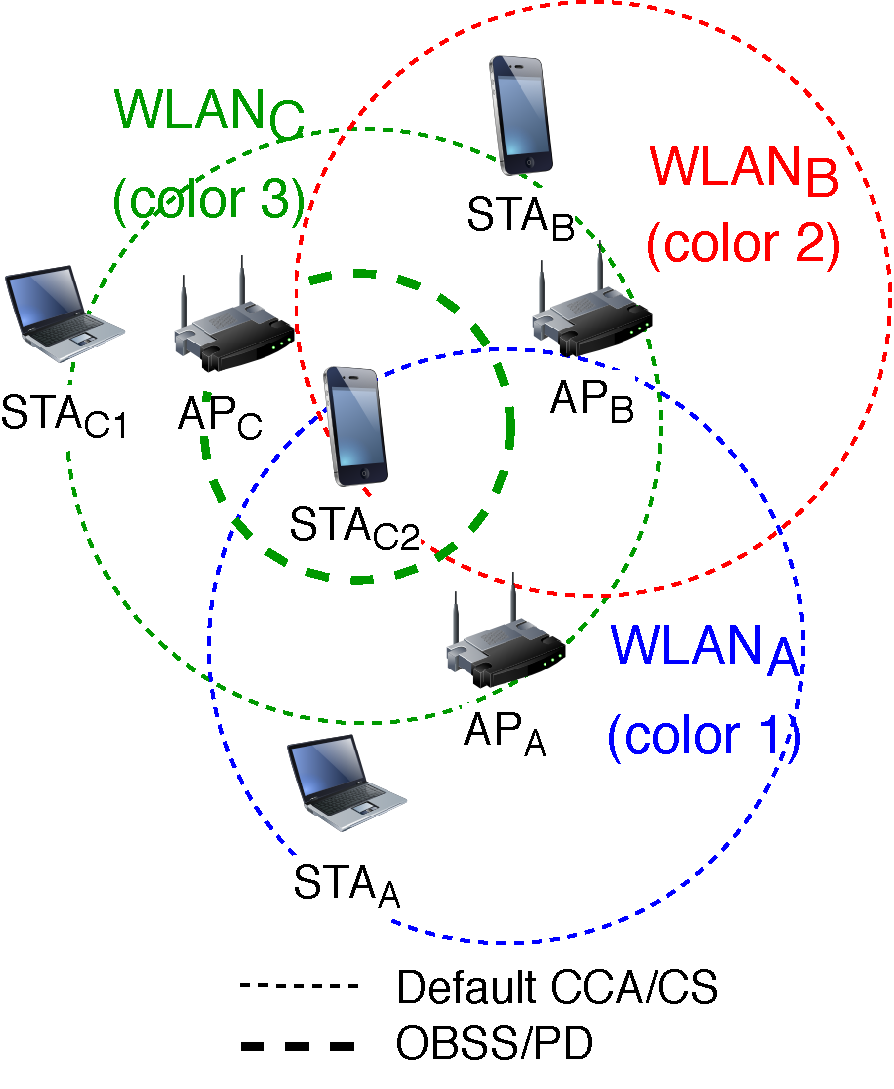
\includegraphics[width=0.6\columnwidth]{fig_11}
		\caption{Scenario for showcasing the OBSS/PD SR operation.}
		\label{fig:fig_8_a}
	\end{figure}
	
	The OBSS/PD-based SR operation can solve the flow starvation issue experienced in $\text{STA}_\text{C2}$ by allowing the latter to ignore inter-BSS transmissions. In that case, $\text{STA}_\text{C2}$ is able to detect SR opportunities when nodes from $\text{WLAN}_A$ and $\text{WLAN}_B$ transmit, provided that the appropriate OBSS/PD value is used. Notice that any detected SR opportunity is subject to a power restriction. Since different OBSS/PD thresholds can be maintained for different inter-BSS transmissions (of SRG and non-SRG type), different power restrictions can be used. This has to be taken into account before transmitting so that the most restrictive limitation is used once channel access is gained.
	
	Fig. \ref{fig:fig_12} illustrates an example of packets exchanged when OBSS/PD-based SR is enabled. The following particular interactions (displayed in yellow) are given:
	\begin{enumerate}
		\item When $\text{AP}_A$ starts transmitting an RTS frame, $\text{STA}_\text{C2}$ analyzes the packet and classifies it as an inter-BSS frame. As a result, it applies a more aggressive CST value, which allows sensing the channel idle ($\text{RSSI}_{A \rightarrow \text{C2}} < \text{OBSS/PD}$). However, $\text{STA}_\text{C2}$ must take into account a first power restriction, which is given by Equation \eqref{eq:power_restriction}.
		\item The same procedure is followed at $\text{STA}_\text{C2}$ when detecting the RTS frame transmitted by $\text{AP}_C$. However, the transmission cannot be ignored this time since a more restrictive PD policy is applied for intra-BSS frames (i.e., default CCA/CS).
		\item As for points 1) and 2), $\text{AP}_B$'s transmission is ignored by $\text{STA}_\text{C2}$ because $\text{RSSI}_{B \rightarrow \text{C2}} < \text{OBSS/PD}$. Again, a new power restriction is considered.
		\item Finally, $\text{STA}_\text{C2}$ is able to transmit because of the detected SR opportunities. The transmission is nonetheless subject to the transmission power limitation, which is the more restrictive one from all the collected power restrictions (PRs). In particular, $\text{TX PWR}_{max} = \min(\text{PR}_1, \text{PR}_2)$.\footnote{Notice that, once $\text{STA}_\text{C2}$ transmits under the power restriction, the ACK sent by $\text{STA}_B$ can be ignored, so that a new power restriction is not defined.}
	\end{enumerate}
	
	\begin{figure}[ht!]
		\centering
		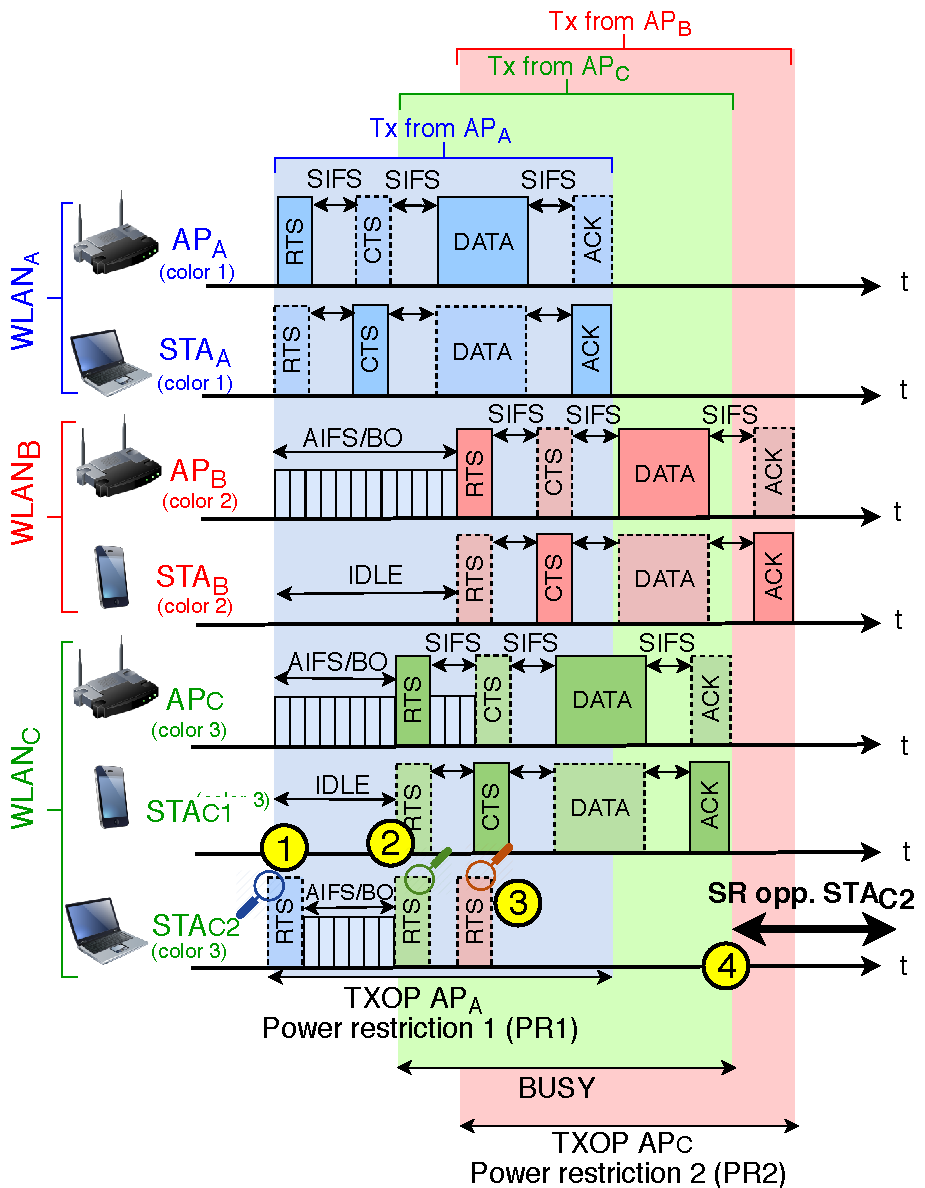
\includegraphics[width=\columnwidth]{fig_12}
		\caption{Example of the OBSS/PD-based SR operation. Station $\text{STA}_\text{C2}$ applies different OBSS/PD values according to the detected transmission.}
		\label{fig:fig_12}
	\end{figure}
	
	%%% SRP-based SR
	\subsection{SRP-based Spatial Reuse}
	\label{section:srp_based}	
	The SRP-based SR operation, in contrast to the OBSS/PD-based one, requires certain cooperation among nodes belonging to different WLANs. In particular, SRP-based SR uses TB communications (see Section \ref{section:tb_communication}) as a building block for identifying opportunities that allow increasing the number of parallel transmissions. Those opportunities, so-called \emph{SRP opportunities}, are detected from TF packets. In case of detecting an SRP opportunity, an HE node can ignore TB PPDU(s) that follow a TF. However, as for OBSS/PD-based SR, a transmit power limitation is maintained during the duration of the TB PPDU(s). This limitation avoids to negatively impact ongoing transmissions.
	
	% SRP opportunities
	\subsubsection{Detecting SRP opportunities}
	The SRP-based SR operation is achieved when nodes belonging to different WLANs cooperate. On the one hand, we find nodes taking advantage of SRP opportunities (i.e., the \emph{opportunists}). These nodes identify SRP opportunities from detected TB transmissions. On the other hand, we find the \emph{transmission holders}, which perform TB transmissions and indicate support for the SRP-based SR operation. Notice that SRP-based opportunities can only be detected from transmission holders that explicitly indicate support for the operation (e.g., in the headers of the TF packet).
	
	When it comes to identifying SRP opportunities, an opportunist must check whether the TB PPDUs that follow a given TF packet can be ignored or not. To do so, the intended transmission power at the opportunist must not exceed the requirements imposed by the transmission holder. Those requirements are encapsulated by the latter through the \texttt{SRP\_INPUT} parameter, which is afterward compared to the intended transmission power of the opportunist. This parameter is indicated in the TF and can take any of the discrete values shown in Table \ref{tbl:sr_subfield_encoding_TB_ppdu}. The SRP INPUT is computed as follows:
	\begin{equation}
	\text{SRP INPUT} = \text{TX PWR}_\text{AP} + \text{I}_\text{AP}^{\max},
	\label{eq:srp_input}
	\nonumber
	\end{equation}
	where $\text{TX PWR}_\text{AP}$ is the normalized transmit power in dBm at the output of the antenna connector, and $\text{I}_\text{AP}^{\max}$ is a normalized value in dB that captures the maximum allowed interference at the transmission holder.\footnote{In particular, $\text{I}_\text{AP}^{\max}$ is computed as the ambient noise plus the interference power level observed at the AP immediately before the TB transmission, plus the SNR margin value (granting a 10\% PER). A safety margin (set by the AP) is also added not to exceed 5 dB.}
	
	\begin{table}[ht!]
		\centering			
		\resizebox{\columnwidth}{!}{
		\begin{tabular}{|c|c|c|c|}
			\hline
			\textbf{Value} & \textbf{Meaning} & \textbf{Value} & \textbf{Meaning} \\ \hline
			0 & SRP\_DISALLOW & 8 & SRP = -44 dBm \\ \hline
			1 & SRP = -80 dBm & 9 & SRP = -41 dBm \\ \hline
			2 & SRP = -74 dBm & 10 & SRP = -38 dBm \\ \hline
			3 & SRP = -68 dBm & 11 & SRP = -35 dBm \\ \hline
			4 & SRP = -62 dBm & 12 & SRP = -32 dBm \\ \hline
			5 & SRP = -56 dBm & 13 & SRP = -29 dBm \\ \hline
			6 & SRP = -50 dBm & 14 & SRP $\geq$ -26 dBm \\ \hline		7 & SRP = -47 dBm & 15 & \begin{tabular}[c]{@{}c@{}}SRP\_AND\_NON-\\ SRG\_OBSS-PD\_\\ PROHIBITED\end{tabular} \\ \hline
		\end{tabular}}
		\caption{Spatial Reuse subfield encoding for Trigger and HE TB PPDU frames \cite{tgax2019draft}.}
		\label{tbl:sr_subfield_encoding_TB_ppdu}
	\end{table}
	
	Once an opportunist inspects the SRP value of the detected TF,\footnote{The SRP can be extracted either from the \texttt{SPATIAL REUSE} field, which is included in the \texttt{Common Info} field of the Trigger frame, or the \texttt{SIG-A SRP} field of the HE TB PPDU.} it uses it to assess whether the intended transmission power is acceptable or not. If so, the opportunist transmits during the duration of the TB PPDU(s) (indicated in the \texttt{Common Info} field). Otherwise, it remains waiting. In particular, the intended transmission power must be below the value of SRP minus the Received Power Level (RPL), which is measured from the legacy portion of the TF (i.e., from PHY headers).
	
	\begin{figure}[ht!]
		\centering
		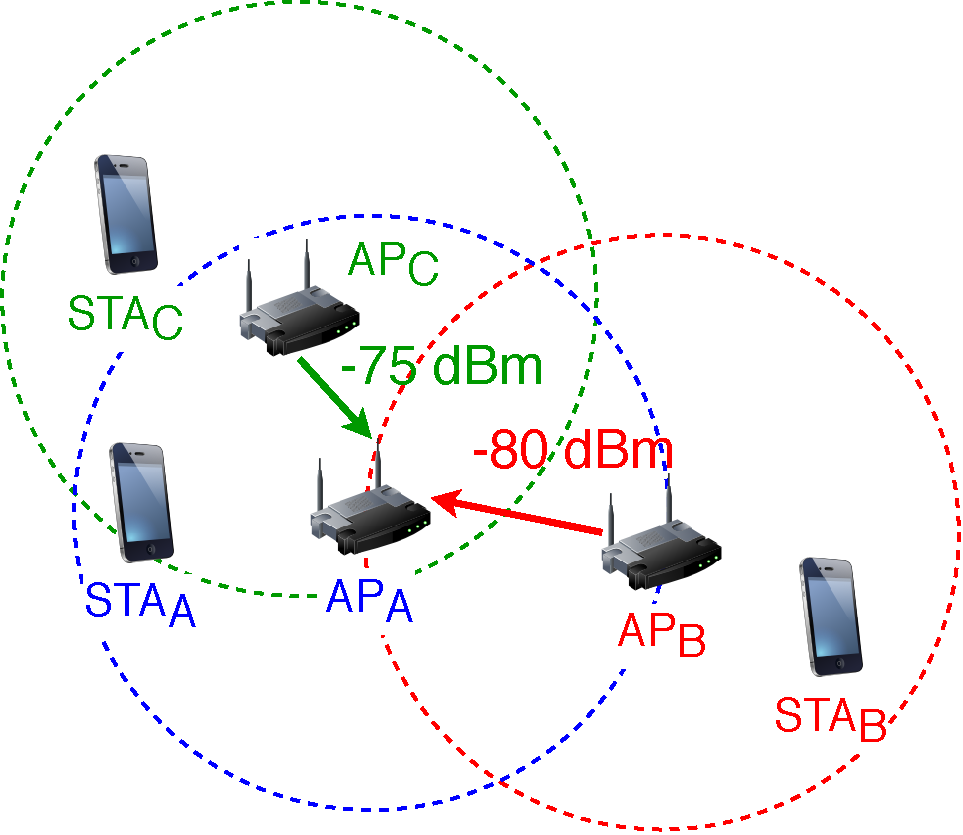
\includegraphics[width=0.65\columnwidth]{fig_13a}
		\caption{Scenario for showcasing the SRP-based SR operation.}
		\label{fig:fig_13a}
	\end{figure}
	
	\begin{figure}[ht!]
		\centering
		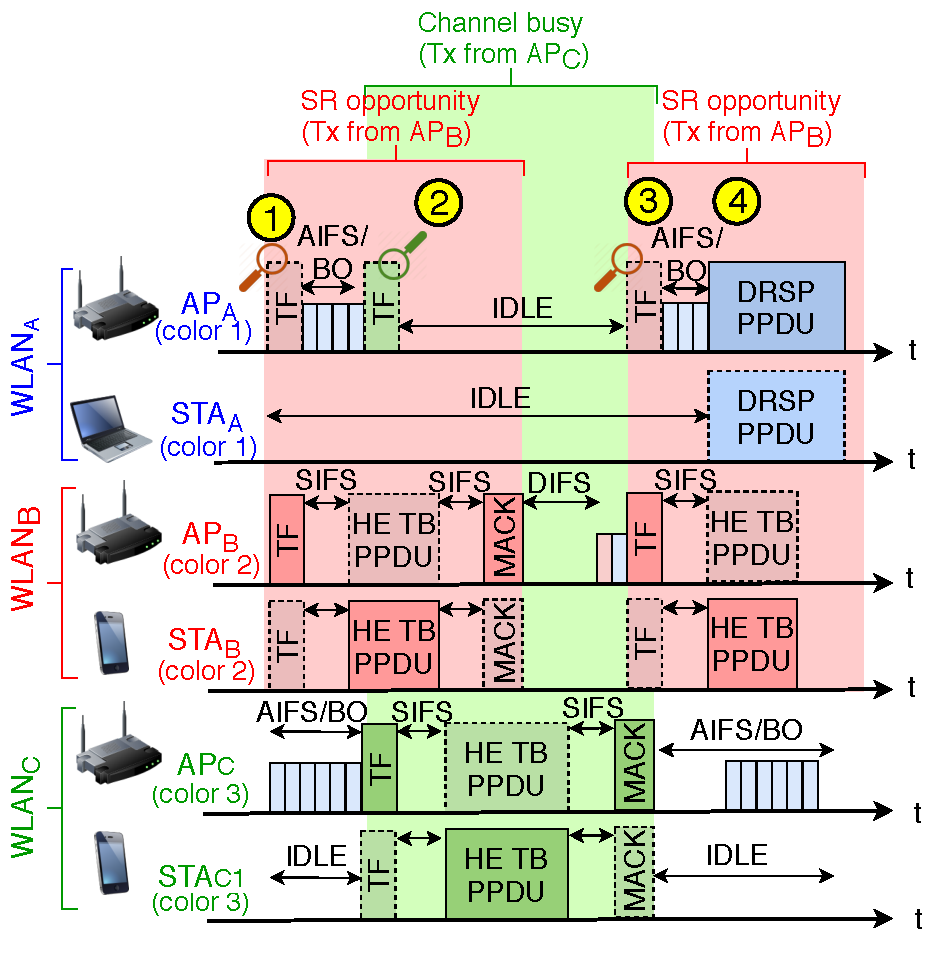
\includegraphics[width=\columnwidth]{fig_13b}
		\caption{Packets exchange according to the SRP-based SR operation.}
		\label{fig:fig_13b}
	\end{figure}
	
	In order to illustrate the SRP-based SR operation, refer to the scenario that is shown in Fig. \ref{fig:fig_13a}, where we focus on $\text{AP}_A$. The interference sensed in that AP from the overlapping transmitters, i.e. $\text{AP}_B$ and $\text{AP}_C$, is -80 dBm and -75 dBm, respectively. According to that, Fig. \ref{fig:fig_13b} shows an example of packets exchange when applying SRP-based SR in $\text{AP}_A$. The actions that are displayed in yellow in the figure are as follows:
	\begin{enumerate}
		\item $\text{AP}_A$ detects an SRP opportunity from $\text{AP}_B$'s TF packet. Notice that the intended transmission power for the next queued packet of $\text{AP}_A$ must be lower than the indicated SRP by $\text{AP}_B$ minus the RPL. If so, $\text{AP}_A$'s backoff keeps counting down.
		\item As soon as $\text{AP}_C$ transmits a TF, the SRP opportunity previously detected by $\text{AP}_A$ is cancelled because the transmission power condition no longer holds. As a result, the channel is now marked as busy and the backoff countdown is frozen.
		\item For a new transmission held by $\text{AP}_B$, an SRP opportunity is detected, even if $\text{WLAN}_C$ is still transmitting. That opportunity may be used by $\text{AP}_A$ as soon as $\text{WLAN}_C$'s transmission finishes.
		\item Once $\text{WLAN}_C$'s transmission is over, $\text{AP}_A$ keeps the backoff countdown and eventually transmits according to the last detected SRP opportunity.
	\end{enumerate}
	
	% ----------------------------------
	% -
	% 	-- Analytical Framework --
	% -
	% ----------------------------------
	
	\section{Model and Simulation of the 11ax Spatial Reuse Operation}
	\label{section:analytical_model}
	%\textcolor{red}{[Incloure un paràgraf breu on s'expliqui la rellevància de contrastar models amb simulacions (assumint que la simulació és acurada) per poder treure conclusions sobre les dinàmiques que passen, i plantejar-se coses que sense fer aquest esforç no es veurien.]}
	
	Characterizing the IEEE 802.11ax SR operation is crucial to fully understand its implications. However, it turns out to be a challenging task due to the complex (and still unknown) inter-WLAN interactions generated by adjusting the sensitivity and the transmission power. To the best of our knowledge, none of the previous works have attempted to model the 11ax SR operation. Nevertheless, with the aim of providing a thorough understanding of the SR operation, we introduce the CSMA/CA throughput model based on Continuous Time Markov Networks (CTMNs) \cite{bellalta2014throughput, bellalta2017throughput}. The analytical model presented in this work aims to provide further insight into the effects of applying SR in next-generation WLANs.
	
	In addition to the analytical model, we introduce the 11ax SR operation in the Komondor \cite{barrachina2019komondor} simulator.\footnote{The implementation of SR can be found in Komondor v3.0, available in \url{https://github.com/wn-upf/Komondor/releases/tag/v3.0}.} This simulator was conceived, among other purposes, to allow the low-cost integration of novel mechanisms included in new IEEE 802.11 standards. This is the case of the 11ax SR operation, which has not been yet fully implemented in any other well-known simulator. To the date of publishing this article, SR is still being developed for ns-3.\footnote{It is planned to be included in the following repository: \url{https://gitlab.com/nsnam/ns-3-dev}.} 
	
	By comparing our simulation results with the analytical model, we expect to shed some light on the effects of using 11ax SR, particularly with regard to inter-WLAN interactions. The analytical model will assist us in drawing conclusions regarding the network dynamics that can occur when applying the SR operation.
	
	Before getting into the analysis of IEEE 802.11ax SR through CTMNs, it is important to mention that we have only modeled the OBSS/PD-based operation described in Section \ref{section:obss_pd_based}. Therefore, from now onwards, we may refer to the OBSS/PD-based SR operation simply as SR operation. Notice that both OBSS/PD-based and SRP-based SR are expected to lead to similar inter-WLAN interactions. The fact is that both mechanisms rely on the same sensitivity and transmission power adjustment procedures. However, the way SR opportunities are detected is different and entails additional complexity for the SRP-based SR case. While OBSS/PD-based SR operates for any incoming transmission, SRP-based SR is activated only for trigger frames. Because of that, the implementation of SRP-based SR is left as future work since it entails the utilization of TB communications, which are not implemented yet in any simulator and are difficult to handle by analytical frameworks. 
	
	\subsection{Introduction to Continuous Time Markov Networks}
	
	The CTMN model captures the CSMA/CA operation used in IEEE 802.11 WLANs through states, which represent the set of WLANs that are active at a given moment. Transitions between states occur when WLANs become active (i.e., they gain access to the medium) or when they abandon the channel (i.e., their transmission is finished). It is worth pointing out some assumptions made by the CTMN model. First, the backoff procedure for accessing the medium is continuous in time. Thus, collisions due to backoff expiring at the same instant are not captured by the model. Second, downlink traffic is considered. Accordingly, the model is focused on finding inter-AP interactions.
	
	For the sake of illustration, let us consider Fig. \ref{fig:ctmn}, which represents the CTMN of a single WLAN, namely $\text{WLAN}_A$. In that CTMN, $s_0$ is the empty state (the channel is idle) and $s_1$ indicates that $\text{WLAN}_A$ is transmitting in a given channel.\footnote{In this work, we consider WLANs using the same frequency channel, which allows focusing on the spatial interactions only.} Regarding the transition rates between states, we find two different types: \emph{i)} AP activates, and \emph{ii)} AP finishes a transmission. While \emph{i)} is related to the necessary time for a given node to access the channel (characterized by the arrival rate $\lambda$), \emph{ii)} depends on the time spent by a given node for transmitting data (characterized by the service rate $\mu$). According to the transitions probabilities, one can obtain the long-term throughput experienced by each WLAN through the probability of being in each state.
	
	\begin{figure}[h!!!!]	
		\centering
		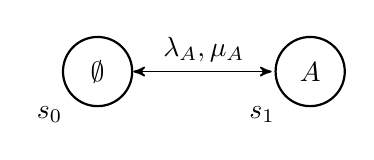
\begin{tikzpicture}[scale=1, align = center, <->,>=stealth',shorten >=1pt,auto,node distance=1.5cm,	semithick]
		\tikzstyle{every state}=[fill=white,draw=black,thick,text=black,scale=1]
		\node[state, label=below left:$s_0$]    (S1)  {$\emptyset$};
		\node[state, label=below left:$s_1$]    (S2)[right of = S1, xshift=1.2cm] {$A$};
		\path
		(S1) edge node[sloped, anchor=center, above]{$\lambda_A,\mu_A$} (S2);
		\end{tikzpicture}
		\caption{CTMN of $\text{WLAN}_A$.} 
		\label{fig:ctmn}
	\end{figure}
	
	In this work, the 11ax SR operation has been implemented as part of the Spatial Flexible Continuous Time Markov Network (SFCTMN) framework \cite{barrachina2019dynamic, barrachina2019overlap, wilhelmi2019potential}.\footnote{A dedicated Github branch of SFCTMN has been provided for single-channel spatial reuse \cite{wilhelmi2019sfctm_spatial_reuse}.} This framework allows generating the CTMN of a given scenario, according to the spatial distribution of nodes and their configuration (e.g., range of channels used, transmission power, sensitivity, etc.). It is important to highlight that additive interference is considered, which results from the combination of different simultaneous interfering transmissions. Accordingly, we are able to characterize real deployments where spatially-distributed interactions occur. Moreover, traffic is considered to be saturated in all the nodes, so that pure SR-based interactions become more apparent.
	
	In order to model the 11ax SR operation, we have considered the generation of new states, which are related to the different sensitivity levels that each WLAN can use. Notice that using different sensitivity levels enables, on the one hand, to find new types of inter-WLAN interactions that could not exist without applying SR. On the other hand, increasing the sensitivity entails decreasing the transmission power. As a result, the capabilities of a given node vary according to the OBSS/PD threshold that is employed in every situation; a lower transmission power entails using a more robust Modulation and Coding Scheme (MCS). 
	
	%%% Simple OBSS/PD-based interactions
	\subsection{Simple inter-WLAN interactions}
	\label{section:simple_interactions}
	
	We first focus on simple inter-WLAN interactions that occur when applying the SR operation. With that aim, we start introducing a very simple scenario (namely, \emph{Toy scenario 1}), where two WLANs coexist, but only $\text{WLAN}_A$ implements SR. Fig. \ref{fig:cs_toy_scenario_1a} and Fig. \ref{fig:cs_toy_scenario_1b} illustrate the default and the spatial reuse operation in \emph{Toy scenario 1}, respectively. In both cases, we show the carrier sense area of each transmitter with respect to the other one. The CTMNs that depicts the inter-WLAN interactions taking place in each case are depicted in Fig. \ref{fig:ctmn_toy_scenario_1a} and Fig. \ref{fig:ctmn_toy_scenario_1b}, respectively. Notice that we show the long-term probability of each state in parentheses.
	
	\begin{figure}[h!]
		\centering
		% Situation 1
		\subfigure[Sensing area]{\label{fig:cs_toy_scenario_1a}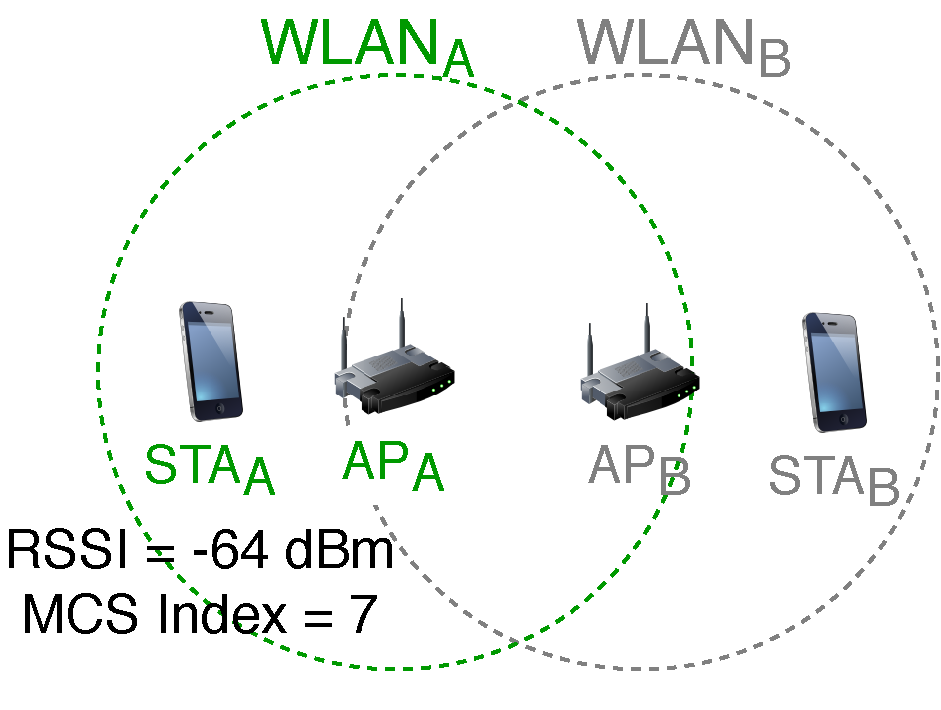
\includegraphics[width=0.2\textwidth]{fig_15a}}
		% CTMN 1
		\subfigure[CTMN]{ \scalebox{0.6}{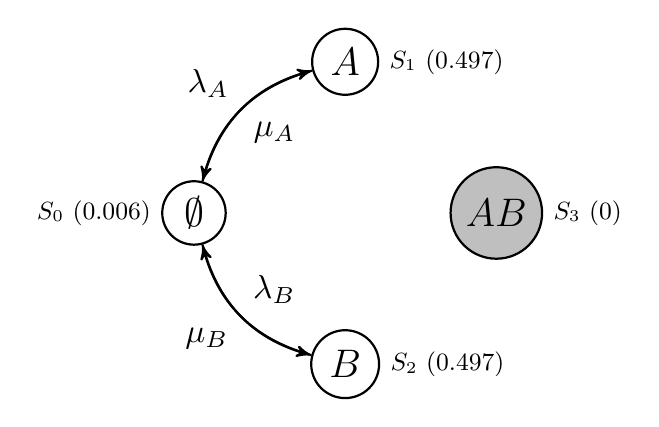
\begin{tikzpicture}[->,>=stealth',shorten >=0.5pt,auto,node distance=1.92cm,thick,main node/.style={circle,draw,font=\sffamily\Large\bfseries}]
			\tikzstyle{every state}=[fill=white,draw=black,thick,text=black,scale=1]	% Nodes
			\node[main node] (1) [label={right:\small $S_1$ (0.497)}] {$A$};
			\node[main node] (2) [label=left:{\small $S_0$ (0.006)}] [left of=1, below of=1] {$\emptyset$};
			\node[main node] (3) [label={right:\small $S_2$ (0.497)}] [right of=2, below of=2] {$B$};
			\node[main node, fill=lightgray] (4) [label=right:{\small $S_3$ (0)}] [right of=1, below of=1] {$AB$};
			% Arrows
			\path[every node/.style={scale=1.2}]
			(1) edge [bend right] node {$\mu_A$} (2)
			(2) edge [bend left] node {$\lambda_A$} (1)
			(3) edge [bend left] node {$\mu_B$} (2)
			(2) edge [bend right] node {$\lambda_B$} (3);	\label{fig:ctmn_toy_scenario_1a}
			\end{tikzpicture}}}\\
		% Situation 2
		\subfigure[Sensing area]{\label{fig:cs_toy_scenario_1b}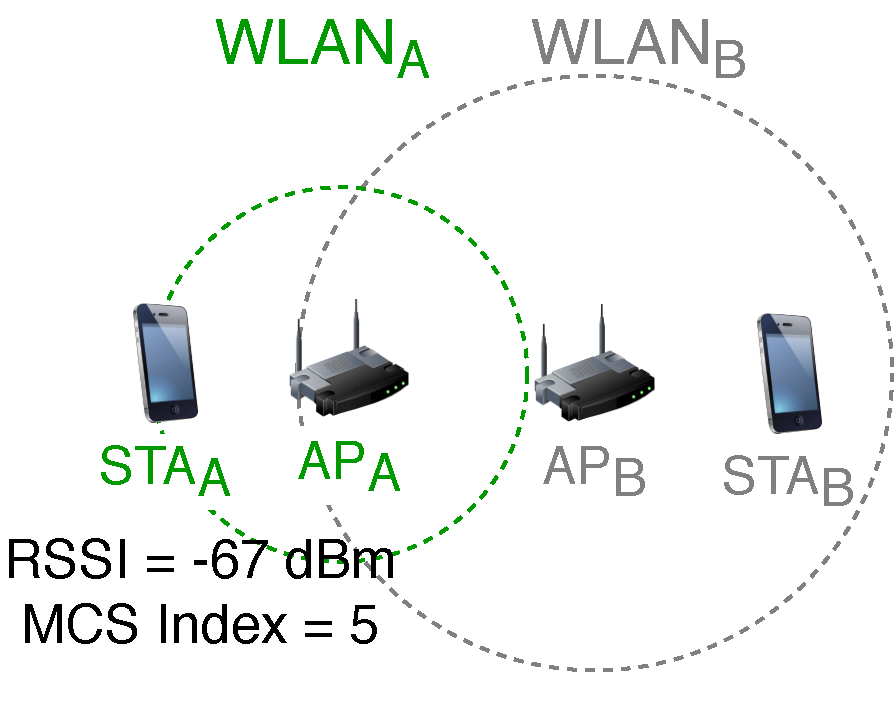
\includegraphics[width=0.2\textwidth]{fig_15c}}%\\
		% CTMN 2
		\subfigure[CTMN]{ \scalebox{0.6}{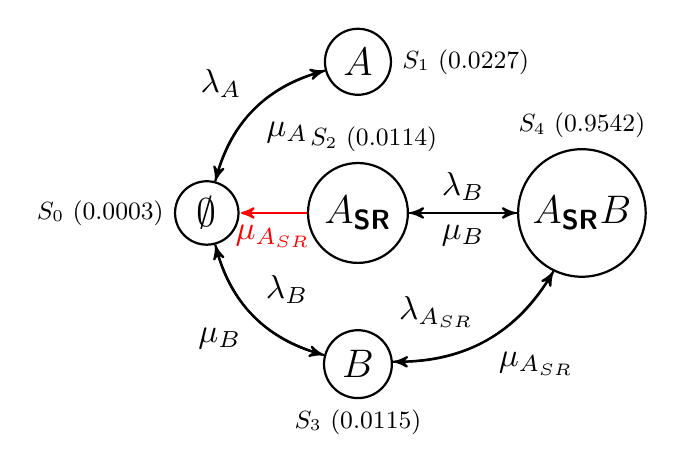
\begin{tikzpicture}[->,>=stealth',shorten >=0.5pt,auto,node distance=1.92cm,thick,main node/.style={circle,draw,font=\sffamily\Large\bfseries}]
			\tikzstyle{every state}=[fill=white,draw=black,thick,text=black,scale=1]	% Nodes
			\node[main node] (1) [label={right:\small $S_1$ (0.0227)}] {$A$};
			\node[main node] (2) [label={above,right=2mm:\small $S_2$ (0.0114)}] [below of=1] {$A_\text{SR}$};
			\node[main node] (3) [label=left:{\small $S_0$ (0.0003)}] [left of=2] {$\emptyset$};
			\node[main node] (5) [label={below:\small $S_3$ (0.0115)}] [below of=2] {$B$};
			\node[main node] (4) [label=above:{\small $S_4$ (0.9542)}] [right of=2, right=1mm] {$A_\text{SR}B$};
			% Arrows
			\path[every node/.style={scale=1.2}]
			(1) edge [bend right] node {$\mu_A$} (3)
			(2) edge node {$\lambda_B$} (4)
			(2) edge[red] node {$\mu_{A_{SR}}$} (3)
			(3) edge [bend left] node {$\lambda_A$} (1)
			(3) edge [bend right] node {$\lambda_B$} (5)
			(4) edge node {$\mu_B$} (2)
			(4)	edge [bend left] node {$\mu_{A_{SR}}$} (5)
			(5) edge [bend left] node {$\mu_B$} (3)
			(5) edge [bend right] node {$\lambda_{A_{SR}}$} (4);	\label{fig:ctmn_toy_scenario_1b}
			\end{tikzpicture}}}
		\caption{Representation of \emph{Toy scenario 1 }for different OBSS/PD values. (a) and (c) represent the carrier sense area of each transmitter for OBSS/PD equal to -82 dBm and -78 dBm, respectively. (b) and (d) illustrate the inter-WLAN interactions through CTMNs for OBSS/PD < -79 dBm and OBSS/PD $\geq$ -79 dBm, respectively (unidirectional transitions are marked in red).}
		\label{fig:toy_scenario_1b}
	\end{figure}
	
	On the one hand, the default operation is employed as long as $\text{WLAN}_A$ uses an OBSS/PD value below -79 dBm. As shown in Fig. \ref{fig:cs_toy_scenario_1a}, both APs are in the carrier sense range of one another. Therefore, parallel transmissions are not possible. This can also be noticed in the CTMN representation (see Fig. \ref{fig:ctmn_toy_scenario_1a}), where state $s_3$ (AB) cannot be reached from any other state. Despite sharing the medium, both WLANs can transmit at a high rate because the maximum transmission power is used when accessing the medium. In particular, the STA in $\text{WLAN}_A$ observes an RSSI of -64 dBm, which allows using the MCS 7 for 20 MHz transmissions.
	
	On the other hand, both WLANs can transmit simultaneously through the SR operation, provided that $\text{WLAN}_A$ uses an OBSS/PD value greater or equal than -79 dBm. As shown in Fig. \ref{fig:cs_toy_scenario_1b}, $\text{AP}_A$ reduces its sensitivity area in case of detecting any transmission from $\text{WLAN}_B$. However, having simultaneous inter-WLAN transmissions has a cost, which is paid by $\text{WLAN}_A$ via the transmission power limitation. This limitation results in poorer signal strength at the STA (RSSI = -67 dBm when the transmit power used by AP$_A$ is 17 dBm), thus forcing to use a lower data rate. The SR operation is represented through the CTMN's model in Fig. \ref{fig:ctmn_toy_scenario_1b}, where new states appear (i.e. $s_2$ and $s_4$). These new states capture the situations in which the transmitter of $\text{WLAN}_A$ uses a higher OBSS/PD in order to ignore $\text{WLAN}_B$'s transmissions (mode $A_\text{SR}$ is used, instead of $A$). In particular, state $s_2$ ($A_\text{SR}$) can never be reached from the empty state since $\text{WLAN}_A$ is always expected to transmit under its default operation when the channel is idle.
	
	To sum up, Fig. \ref{fig:toy_scenario_1_results} shows, for each possible OBSS/PD value, the throughput achieved in $\text{WLAN}_A$ and $\text{WLAN}_B$ (left side), as well as the transmission power used by each one (right side).  
	\begin{figure}[ht!]
		\centering
		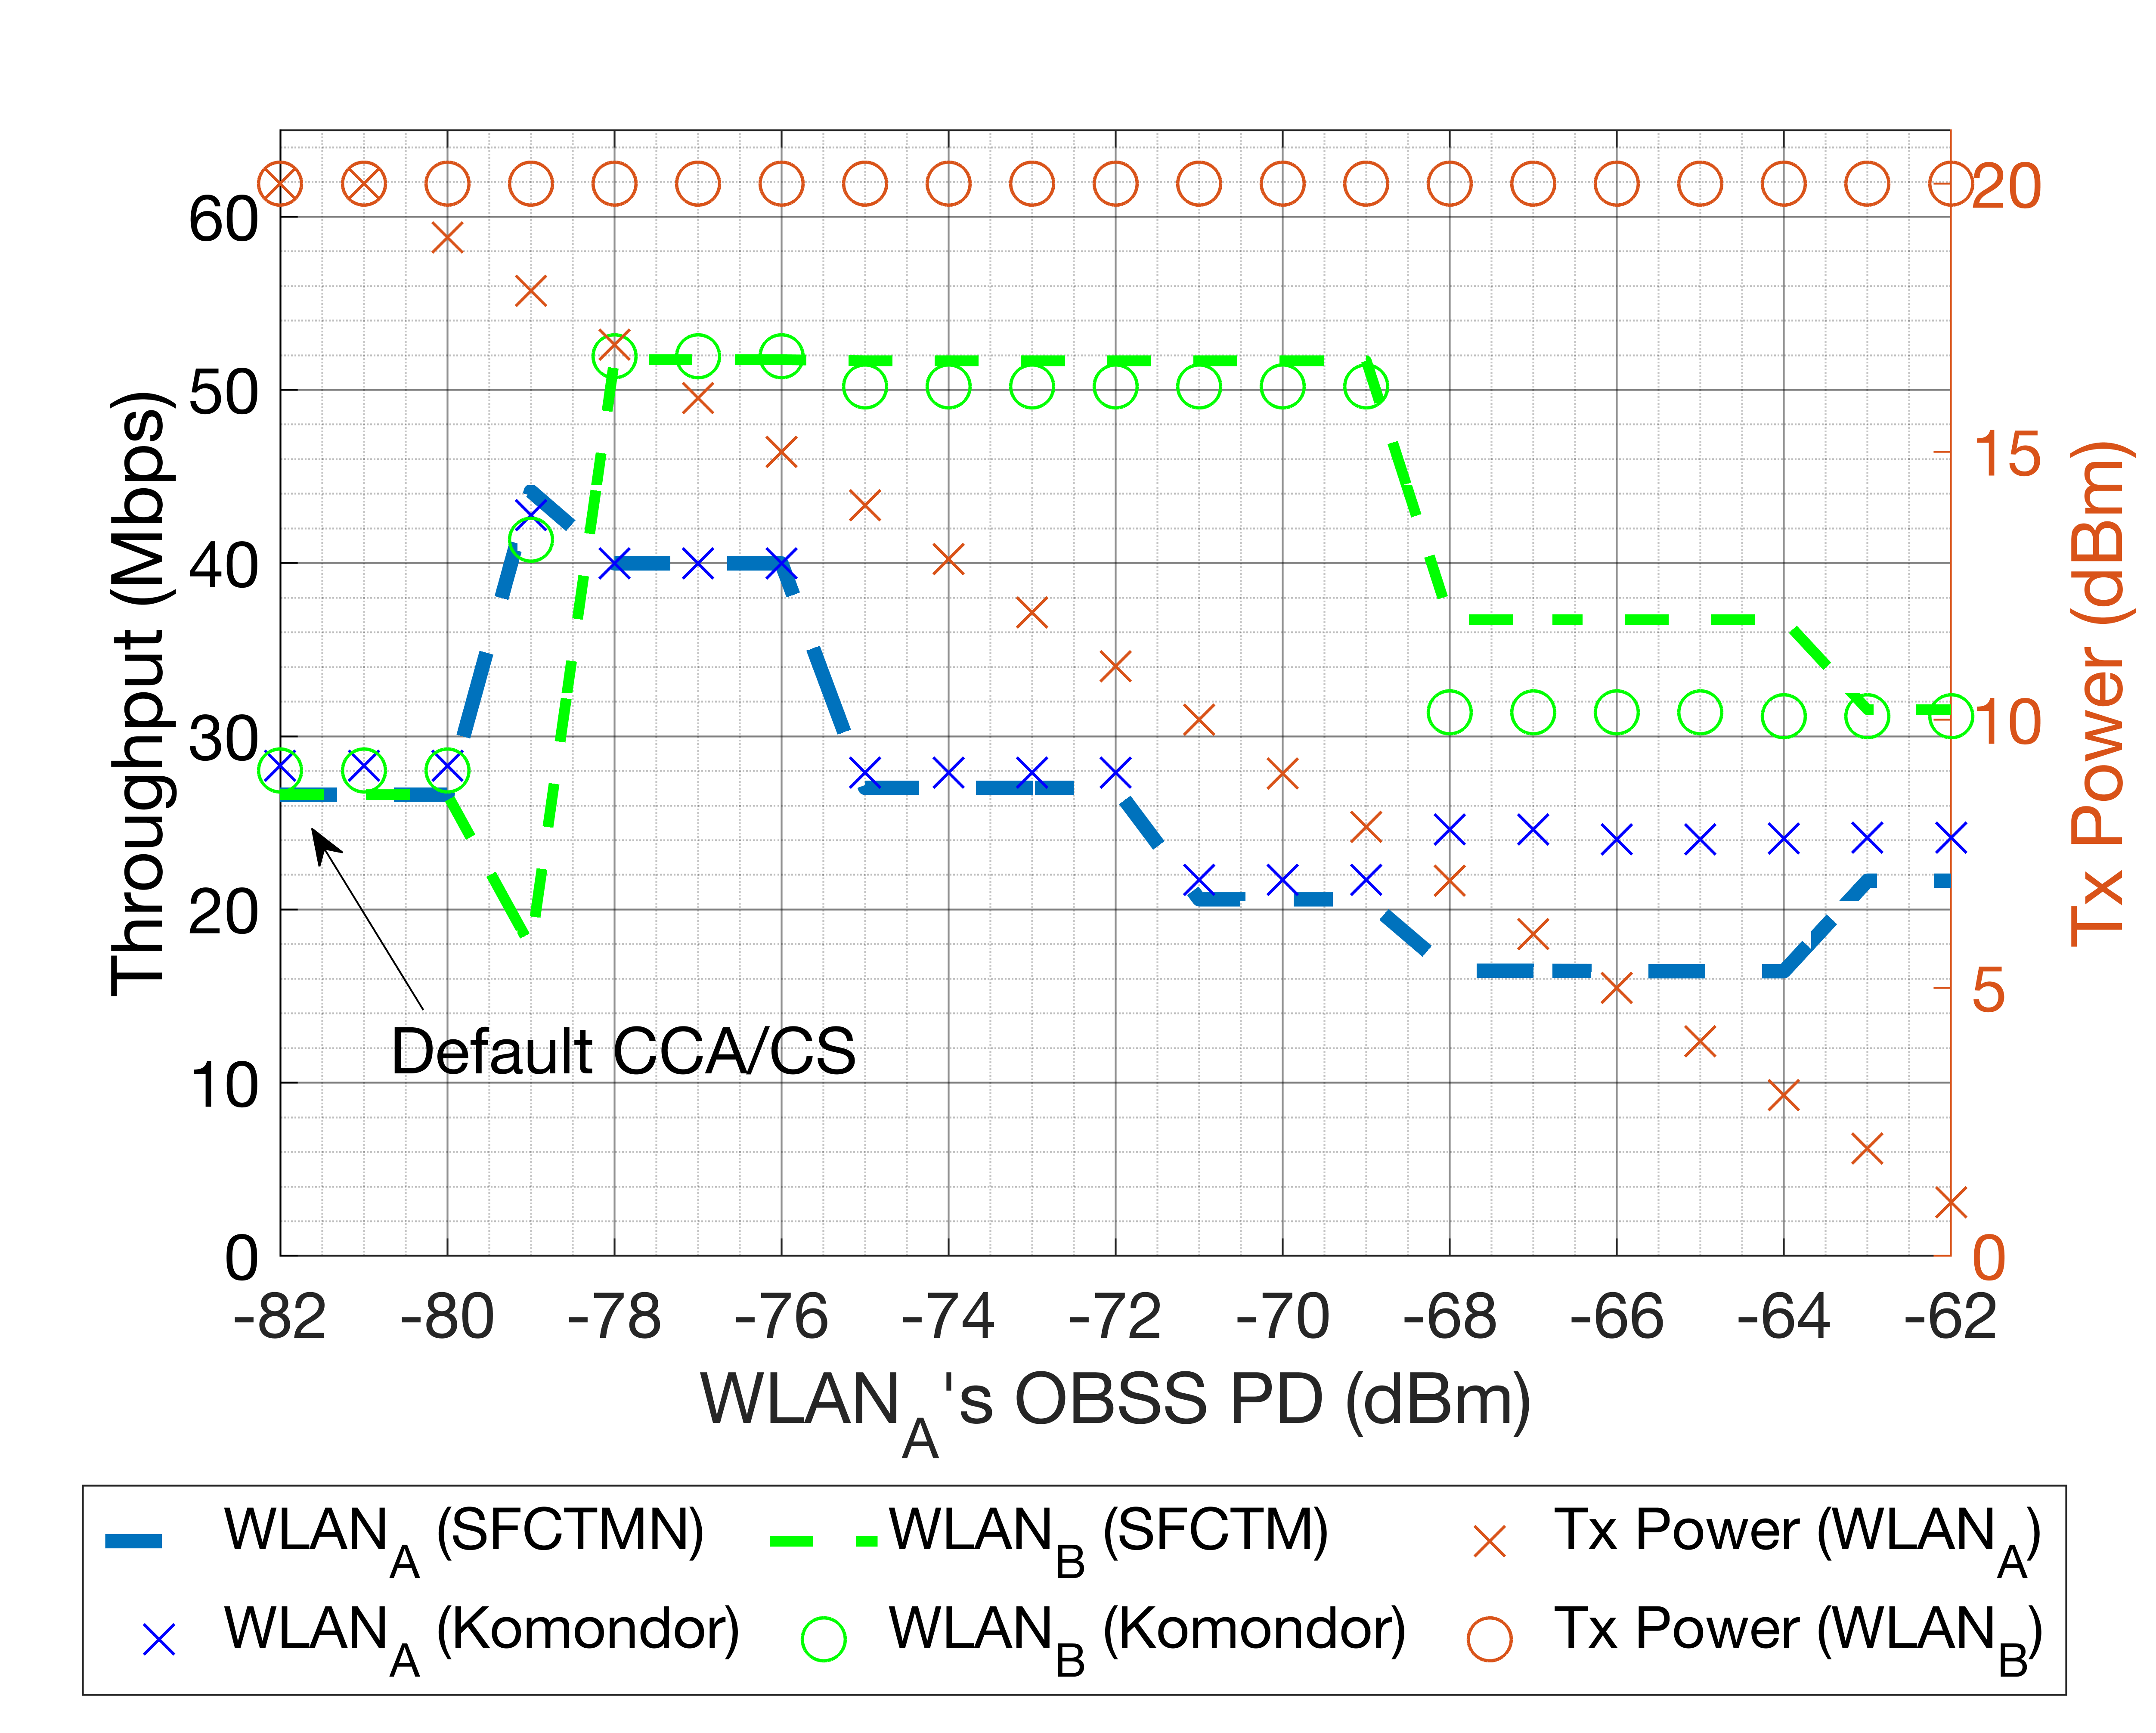
\includegraphics[width=\columnwidth]{SIM_1_1}
		\caption{Effects of applying OBSS/PD-based SR in $\text{WLAN}_A$ of \emph{Toy scenario 1}, for each possible OBSS/PD value. The transmission power is shown in red. Results are shown for both SFCTMN and Komondor.}		\label{fig:toy_scenario_1_results}
	\end{figure}
	
	As shown, both WLANs obtain the same performance for OBSS/PD $<$ -79 dBm (they share the channel). To that point onwards, $\text{WLAN}_A$ is able to ignore $\text{WLAN}_B$'s transmissions due to the SR operation. However, what might seem a worthy strategy for $\text{WLAN}_A$ turns out to be more beneficial to $\text{WLAN}_B$. The latter, except for OBSS/PD = -79 dBm,\footnote{At that point, the transmission power limitation for OBSS/PD = -79 dBm is insufficient. In this case, $\text{WLAN}_B$ senses the channel busy when $\text{WLAN}_A$ transmits under the SR mode.} enjoys the highest possible throughput when $\text{WLAN}_A$ applies the SR operation. The fact is that $\text{WLAN}_A$ is forced to use a lower transmission power in case of transmitting when $\text{WLAN}_B$ is occupying the channel. Therefore, $\text{WLAN}_B$ will keep sensing the channel idle once its transmission finishes, provided that $\text{WLAN}_A$ is still subject to the transmission power restriction.
	
	It is important to note that, in Fig. \ref{fig:toy_scenario_1_results}, there is a region (from OBSS/PD = -68 dBm to OBSS/PD = -64 dBm, both included) in which the SFCTMN is less accurate at capturing the actual OBSS behavior on using SR. In these points, $\text{STA}_A$ cannot decode any transmission from $\text{AP}_A$ in state $A_\text{SR}B$, but it can in the state $A_\text{SR}$. In particular, the transmit power limitation used by $\text{AP}_A$ in the SR mode makes that $\text{STA}_A$ perceives an insufficient signal-to-noise-plus-interference ratio (SINR) when $\text{WLAN}_B$ is also occupying the channel. The main reason is that the SFCTMN model considers that the throughput obtained in every state is independent of the others, and this condition does not hold for states $A_\text{SR}B$ and $A_\text{SR}$. In reality, $\text{AP}_A$ is expected to abandon its transmission in state $A_\text{SR}B$ as soon as a timeout is noticed, thus spending a few time in the SR mode (transition $A_\text{SR}B$ to $A_\text{SR}$ is unlikely). In contrast, the SFCTMN considers that much more time is spent in state $A_\text{SR}$ since transmissions at that point are successful (but slow due to the low MCS used).
	
	\begin{figure}[ht!]
		\centering
		\subfigure[CTMN representation]{ \scalebox{0.6}{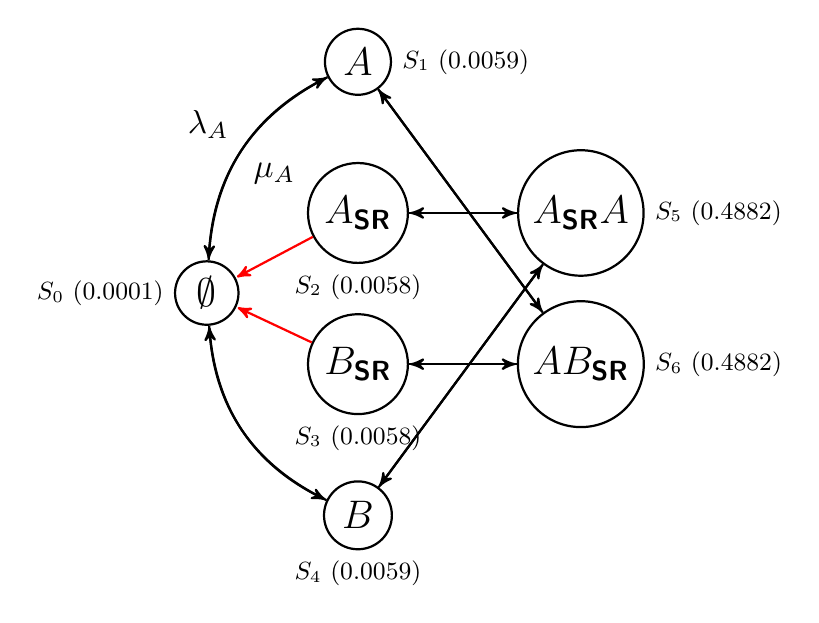
\begin{tikzpicture}[->,>=stealth',shorten >=0.5pt,auto,node distance=1.92cm,thick,main node/.style={circle,draw,font=\sffamily\Large\bfseries}]
			\tikzstyle{every state}=[fill=white,draw=black,thick,text=black,scale=1]	% Nodes
			\node[main node] (1) [label={right:\small $S_1$ (0.0059)}] {$A$};
			\node[main node] (2) [label={below:\small $S_2$ (0.0058)}] [below of=1] {$A_\text{SR}$};
			\node[main node] (3) [label={below:\small $S_3$ (0.0058)}] [below of=2] {$B_\text{SR}$};
			\node[main node] (4) [label=left:{\small $S_0$ (0.0001)}] [left of=2, below=6mm] {$\emptyset$};
			\node[main node] (5) [label={below:\small $S_4$ (0.0059)}] [below of=3] {$B$};
			\node[main node] (6) [label=right:{\small $S_5$ (0.4882)}] [right of=2, right=1mm] {$A_\text{SR}A$};
			\node[main node] (7) [label=right:{\small $S_6$ (0.4882)}] [below of=6] {$AB_\text{SR}$};
			% Arrows
			\path[every node/.style={scale=1.2}]
			(1) edge [bend right] node {$\mu_A$} (4)
			(5) edge [bend left] node {} (4)
			(4) edge [bend left] node {$\lambda_A$} (1)
			(4) edge [bend right] node {} (5)
			(2) edge[red] node {} (4)
			(3) edge[red] node {} (4)
			(1) edge node {} (7)
			(7) edge node {} (1)
			(5) edge node {} (6)
			(6) edge node {} (5)
			(2) edge node {} (6)
			(3) edge node {} (7)
			(6) edge node {} (2)
			(7) edge node {} (3)
			;	\label{fig:ctmn_toy_scenario_1c}
			\end{tikzpicture}}}
		\subfigure[Throughput]{\label{fig:toy_scenario_1c_results}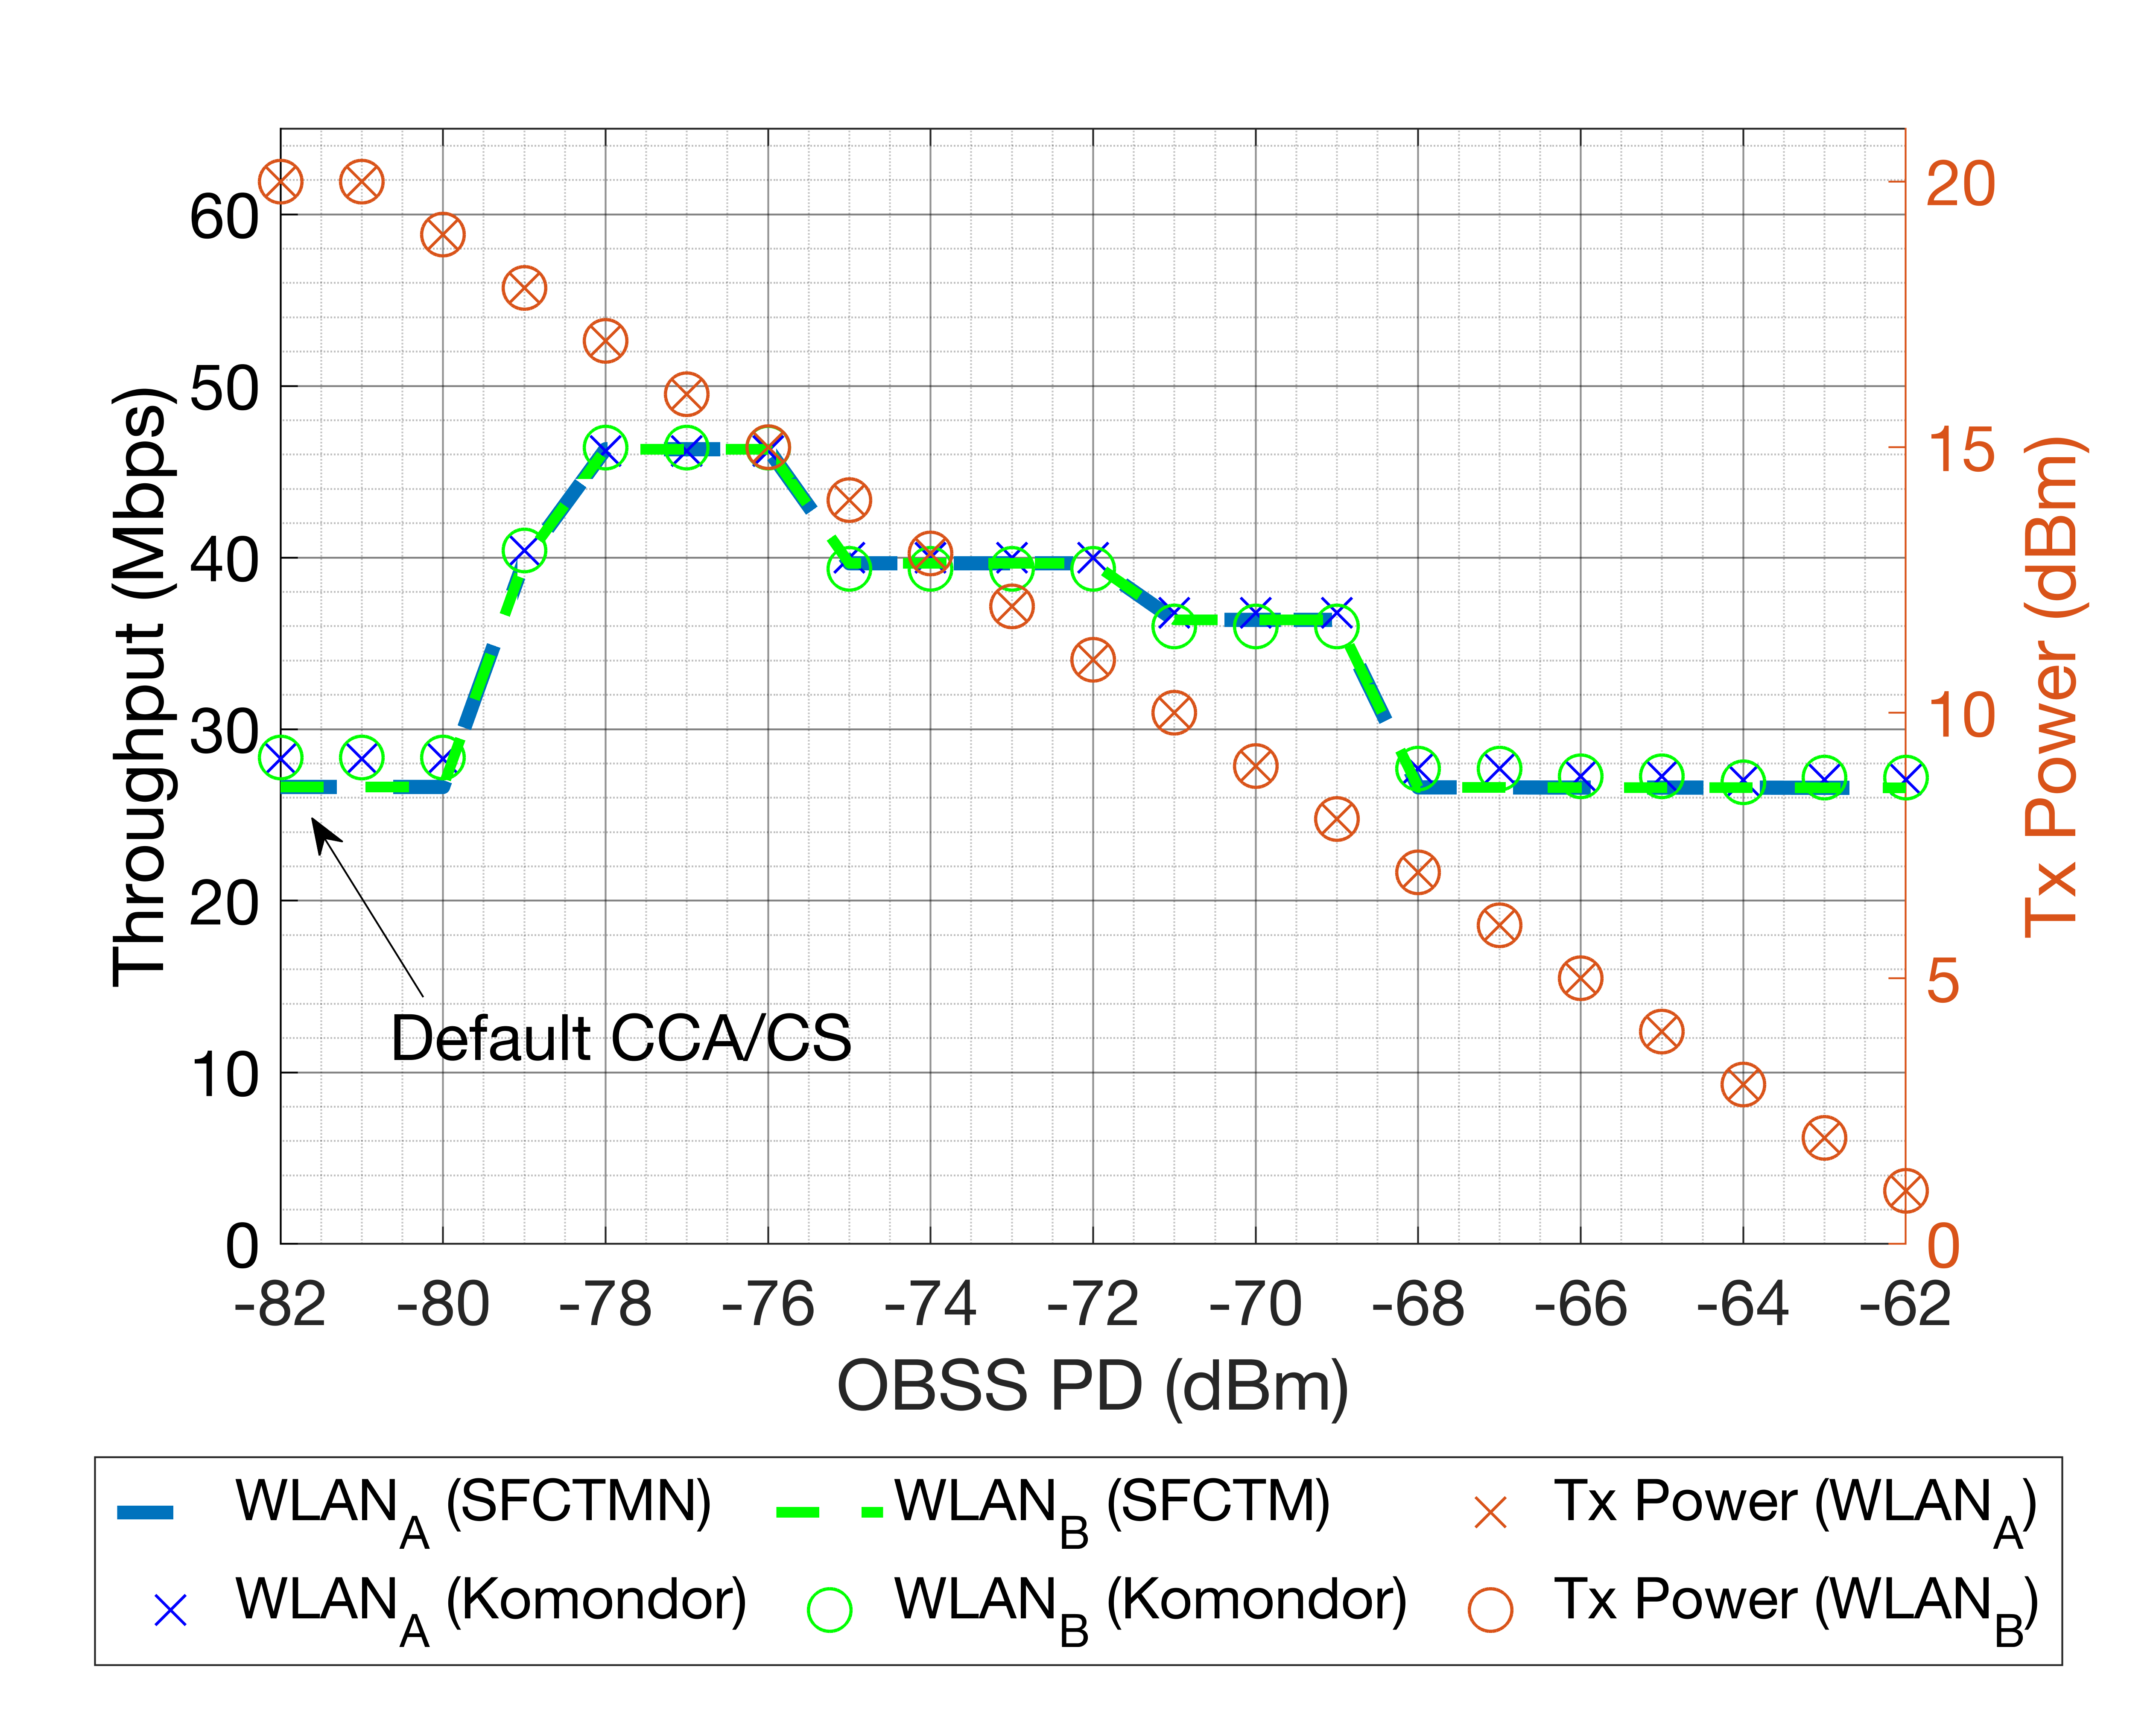
\includegraphics[width=\columnwidth]{SIM_1_1b}}
		\caption{Effects of applying OBSS/PD-based SR in both WLANs of \emph{Toy scenario 1}. (a) CTMN for OBSS/PD~$\geq$~-79~dBm (unidirectional transitions are marked in red), and (b) throughput obtained for each OBSS/PD value. In (b), the transmission power is shown in red, and results are shown for both SFCTMN and Komondor.}
		\label{fig:toy_scenario_1c}
	\end{figure}
	
	Now, let us consider the case where both WLANs apply the SR operation simultaneously. The CTMN for OBSS/PD $\geq$ -79 dBm is illustrated in Fig. \ref{fig:ctmn_toy_scenario_1c}. For the sake of illustration, only transitions between states $s_0$ and $s_1$ are provided. As shown, both WLANs can act by using the default or the SR modes, thus generating a symmetric CTMN. In particular, we find two dominant states: $s_5$  and $s_6$. These states are visited with the same probability (0.4482), which entails that both WLANs alternate the default with the SR mode, thus obtaining the same throughput. However, in reality, one of the WLANs can monopolize the channel through the default mode, so that the other operates under the transmit power-constrained SR mode.
	
	This is what actually occurs in the Komondor simulator, where SR opportunities are identified on a per-packet basis. In this case, the WLAN that accesses to the channel for the first time (e.g., $\text{WLAN}_A$) is most likely to enjoy the maximum throughput. In contrast, the other WLAN (e.g., $\text{WLAN}_B$) transmits under the SR mode almost all the time (as a result of $\text{WLAN}_A$'s activity), until they alternate roles. Notice that a single state between $s_5$  and $s_6$ is more likely to be monopolized as the transmission time becomes longer than the idle periods. In our case, we have very long transmission times in comparison to the idle time since we assume full-buffer traffic, packet aggregation, and short contention window (CW) values.
	
	Fig. \ref{fig:toy_scenario_1c_results} shows the performance achieved by each WLAN when both apply SR, and for each OBSS/PD threshold. The results have been extracted from both SFCTMN and Komondor. In order to show the long-term performance of each WLAN in the Komondor simulator, we have displayed the average values obtained from 100 simulations.
	
	From the long-term performance, we can observe that both WLANs always experience the same throughput, due to the symmetry of the scenario. In particular, states in which SR is used are alternated, thus allowing each WLAN to access the channel while the other is transmitting. As a result, the throughput of both WLANs can be further increased with respect to the case in which only one WLAN applies SR. However, unlike the previous case, the long-term throughput never reaches the maximum possible throughput in isolation (the transmission power limitation prevents to do so).
	
	%%% Complex OBSS/PD-based interactions
	\subsection{Interactions among Spatial Reuse groups}
	\label{section:advanced_interactions}
		
	Differentiating between SRGs may potentially enhance spectral efficiency since further inter-AP interactions can be generated by using an extra PD threshold. In practice, devices belonging to the same SRG use a dedicated OBSS/PD threshold, namely SRG OBSS/PD. For the rest of inter-WLAN transmissions, the non-SRG OBSS/PD threshold is used instead. One possible use case may lie in residential building apartments, where WLANs belonging to the same building form an SRG. For the rest of networks (e.g., public Wi-Fi in the street), other SRGs can be considered.
	
	In order to illustrate the implications of using SR based on SRGs, let us focus on \emph{Toy scenario 2}, which is depicted in Fig. \ref{fig:toy_scenario_2}. In this scenario, all the WLANs apply the SR operation and two different SRGs are created. In particular, WLANs belonging to the same SRG (i.e., $\text{WLAN}_A$ and $\text{WLAN}_B$) are close to each other, such as in a residential building. Besides that, we find $\text{WLAN}_C$, which is part of another SRG. 
	
	The result of jointly applying OBSS/PD-based SR in \emph{Toy scenario 2} is illustrated in Fig. \ref{fig:SIM_1_3_individual}, which plots the throughput achieved by each of the three WLANs, for each combination of SRG and non-SRG OBSS/PD thresholds. Notice that we have considered that all the WLANs use the same PD values since the number of total combinations grows exponentially and is unfeasible to be plotted.
	
	\begin{figure}[ht!]
		\centering
		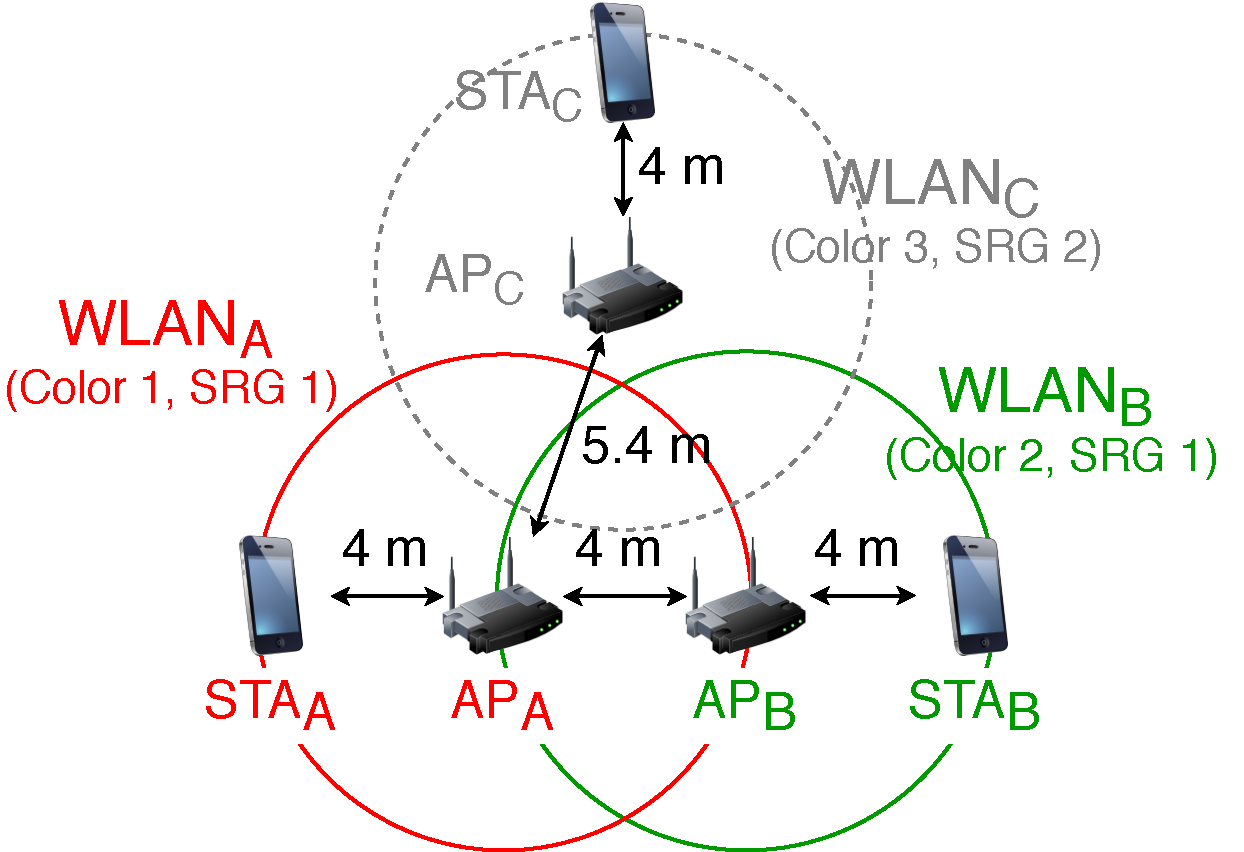
\includegraphics[width=0.8\columnwidth]{fig_18}
		\caption{Toy scenario 2.}
		\label{fig:toy_scenario_2}
	\end{figure}

	\begin{figure}[ht!]
		\centering
		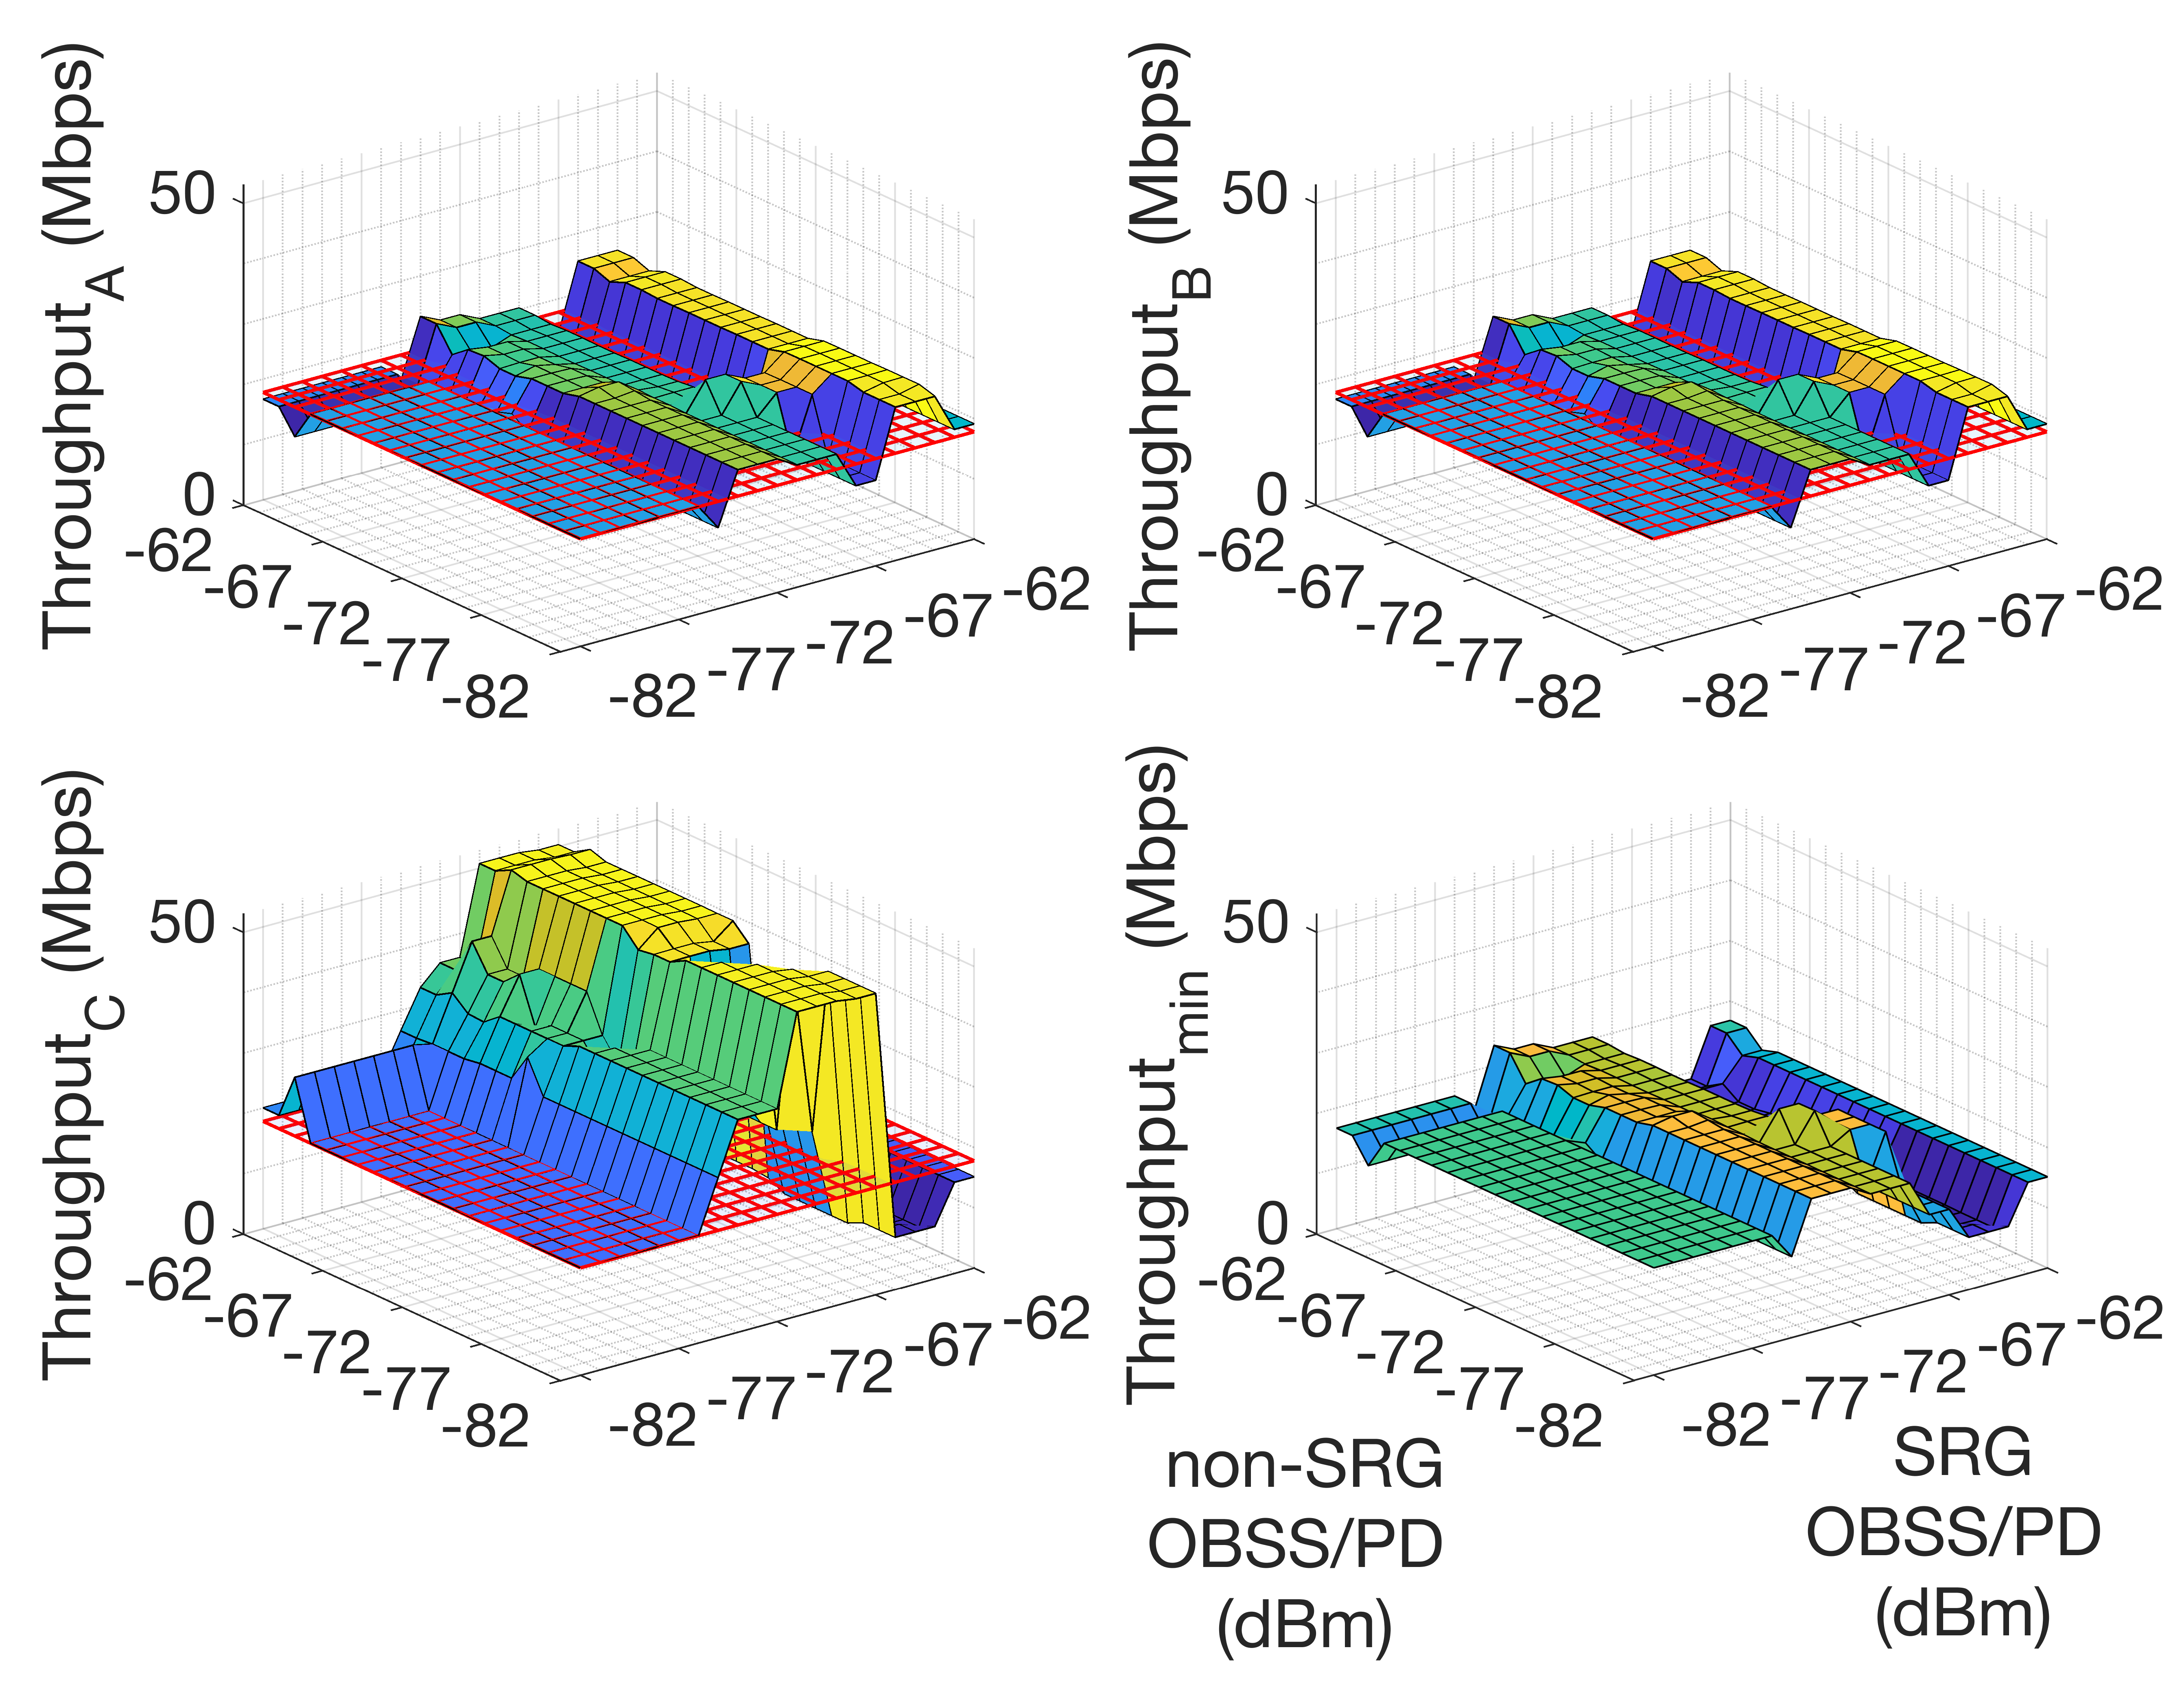
\includegraphics[width=\columnwidth]{SIM_1_2}
		\caption{Individual and max-min throughput achieved in \emph{Toy scenario 2}, for each SRG and non-SRG OBSS/PD threshold. The red mesh indicates the performance achieved by using the default CCA/CS.}
		\label{fig:SIM_1_3_individual}
	\end{figure}
	
	As shown, the throughput achieved by each WLAN follows an irregular pattern due to the complex inter-WLAN interactions that take place in this scenario. Moreover, it can be appreciated the clashing interests of each WLAN, where the individual performance is sometimes maximized at the expense of reducing the throughput of the others. For instance, if we focus on $\text{WLAN}_C$, it obtains the maximum throughput when flow starvation is generated to $\text{WLAN}_A$ (the same occurs for $\text{WLAN}_B$). The CTMN that results of that situation is shown in Fig. \ref{fig:ctmn_scenario_2}, which is given when all the WLANs use non-SRG OBSS/PD = -82 dBm and SRG OBSS/PD = -73 dBm.\footnote{The CTMN model captures the utilization of different OBSS/PD thresholds by considering that each WLAN acts in three different ways (states), according to the PD threshold that employs: \emph{i)} default CCA/CS, \emph{ii)} SRG OBSS/PD, and \emph{iii)} non-SRG OBSS/PD.}
	
	However, that solution is not optimal in terms of fairness. If we consider the optimal max-min performance\footnote{The max-min throughput corresponds to the solution that maximizes the minimum throughput achieved by a set of WLANs.}, a completely different solution is obtained. In this case, the max-min throughput is increased when every WLAN can overtake a single detected inter-BSS transmission (regardless of its source) and access to the channel. This situation is fair and at the same time increases the overall performance. However, it occurs when all the inter-BSS transmissions are equally treated. Using SRGs can therefore improve the performance of certain nodes (belonging to the same group), but potentially leads to unfairness. 
	
	\begin{figure}[ht]
		\centering
		\scalebox{0.65}{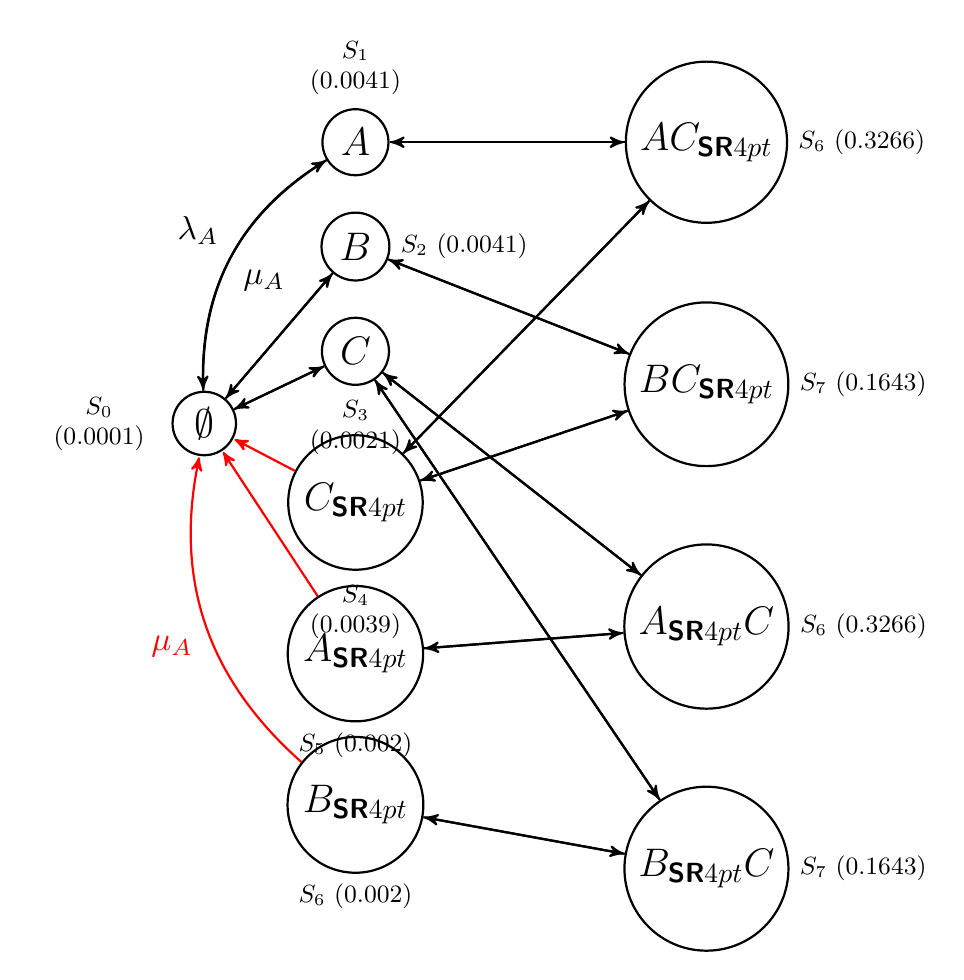
\begin{tikzpicture}[->,>=stealth',shorten >=0.5pt,auto,node distance=1.92cm,thick,main node/.style={circle,draw,font=\sffamily\Large\bfseries}]
			\tikzstyle{every state}=[fill=white,draw=black,thick,text=black,scale=1]	% Nodes
			% States with 1 or none WLANs
			\node[main node] (1) [label={above:\small \begin{tabular}{c}$S_1$ \\(0.0041)\end{tabular}}] {$A$};
			\node[main node] (2) [label={right:\small $S_2$ (0.0041)}] [below of=1, above=1.5mm] {$B$};
			\node[main node] (3) [label={below:\small \begin{tabular}{c}$S_3$ \\(0.0021)\end{tabular}}] [below of=2, above=1.5mm] {$C$};
			\node[main node] (4) [label=left:{\small \begin{tabular}{c}$S_0$ \\(0.0001)\end{tabular}}] [left of=3, below=5mm] {$\emptyset$};
			\node[main node] (5) [label={below:\small \begin{tabular}{c}$S_4$ \\(0.0039)\end{tabular}}] [below of=3] {$C_{\scaleto{\text{SR}}{4pt}}$};
			\node[main node] (6) [label={below:\small $S_5$ (0.002)}] [below of=5] {$A_{\scaleto{\text{SR}}{4pt}}$};
			\node[main node] (7) [label={below:\small $S_6$ (0.002)}] [below of=6] {$B_{\scaleto{\text{SR}}{4pt}}$};
			% Combinations of WLANs
			\node[main node] (8) [label=right:{\small $S_6$ (0.3266)}] [right of=1, right=15mm] {$AC_{\scaleto{\text{SR}}{4pt}}$};
			\node[main node] (9) [label=right:{\small $S_7$ (0.1643)}] [below of=8, below=1mm] {$BC_{\scaleto{\text{SR}}{4pt}}$};
			\node[main node] (10) [label=right:{\small $S_6$ (0.3266)}] [below of=9, below=1mm] {$A_{\scaleto{\text{SR}}{4pt}}C$};
			\node[main node] (11) [label=right:{\small $S_7$ (0.1643)}] [below of=10, below=1mm] {$B_{\scaleto{\text{SR}}{4pt}}C$};
			% Arrows
			\path[every node/.style={scale=1.2}]
			(1) edge [bend right] node {$\mu_A$} (4)
			(2) edge node {} (4)
			(3) edge node {} (4)
			(5) edge [red] node {} (4)
			(6) edge [red] node {} (4)
			(7) edge [red, bend left] node {$\mu_A$} (4)
			(4) edge [bend left] node {$\lambda_A$} (1)
			(4) edge node {} (2)
			(4) edge node {} (3)
			
			(1) edge node {} (8)
			(8) edge node {} (1)
			(2) edge node {} (9)
			(9) edge node {} (2)
			(3) edge node {} (10)
			(10) edge node {} (3)
			(3) edge node {} (11)
			(11) edge node {} (3)
			
			(5) edge node {} (8)
			(8) edge node {} (5)
			(5) edge node {} (9)
			(9) edge node {} (5)
			
			(6) edge node {} (10)
			(10) edge node {} (6)
			(7) edge node {} (11)
			(11) edge node {} (7)
			;
			\end{tikzpicture}}
		\caption{CTMN of \emph{Toy scenario 2}, for non-SRG OBSS/PD = -73 dBm and SRG OBSS/PD = -82 dBm. The unidirectional transitions are marked in red, and subindex \emph{SR} indicates the use of the non-SRG OBSS/PD threshold.}
		\label{fig:ctmn_scenario_2}
	\end{figure}
	
	Table \ref{tbl:cross_validation} provides a verification, for both SFCTMN and Komondor, of the results obtained in \emph{Toy scenario 2}. For the sake of representation, we show the Root Mean Square Error (RMSE) for all the SRG and non-SRG OBSS/PD thresholds. As shown, the error for $\text{WLAN}_A$ and $\text{WLAN}_B$ is relatively small. In contrast, a higher error is obtained for $\text{WLAN}_C$. This is strongly related to the fact that $\text{WLAN}_C$ belongs to a different SRG than $\text{WLAN}_A$ and $\text{WLAN}_B$, which is expected to generate more inter-WLAN interactions. Moreover, dominant states may lead to situations that cannot be captured by the SFCTMN, as previously shown for \emph{Toy scenario 1}. In particular, $\text{WLAN}_C$ in \emph{Toy scenario 2} is prone to participate in these states because of its asymmetric location with respect to $\text{WLAN}_A$ and $\text{WLAN}_B$.
	%Notice that SFCMTN only considers inter-AP interactions for generating states. However, despite the traffic is considered to be in the downlink, in Komondor STAs spend some time transmitting (basically, acknowledgments). These short transmissions intervals entail some important inter-WLAN interactions that are not captured by the SFCTMN. Moreover, the SFCTMN neither contemplates the simultaneous transmissions that can occur in case that two or more transmitters choose the same backoff value. Nevertheless, they can happen in reality, especially for short CW and high traffic load. 
	
	\begin{table}[]
		\centering
		\begin{tabular}{|c|l|c|c|c|}
			\hline
			\multicolumn{2}{|c|}{\multirow{2}{*}{\textbf{}}} & \multicolumn{3}{c|}{\textbf{WLAN}} \\ \cline{3-5} 
			\multicolumn{2}{|c|}{} & \textit{A} & \textit{B} & \textit{C} \\ \hline
			\multicolumn{2}{|c|}{\begin{tabular}[c]{@{}c@{}}RMSE\\ (Mbps)\end{tabular}} & 6.02 & 6.03 & 18.42 \\ \hline
		\end{tabular}
		\caption{Verification of the results obtained in \emph{Toy scenario 2} from the SFCTMN model and Komondor.}
		\label{tbl:cross_validation}
	\end{table}
	
	% ----------------------------------
	% -
	% 	-- Performance Evaluation --
	% -
	% ----------------------------------
	
	\section{Performance Evaluation}
	\label{section:performance_evaluation}

	In this Section, we aim to show the potential of applying SR by using large-scale WLAN scenarios. With this aim, we leave the CTMNs-based analysis out and concentrate on simulation results. For the rest of this Section, WLANs are considered to be composed by an AP and a single STA, which are placed uniformly at random, as shown in Fig. \ref{fig:random_scenario}. 
	
	\begin{figure}[ht!]
		\centering
		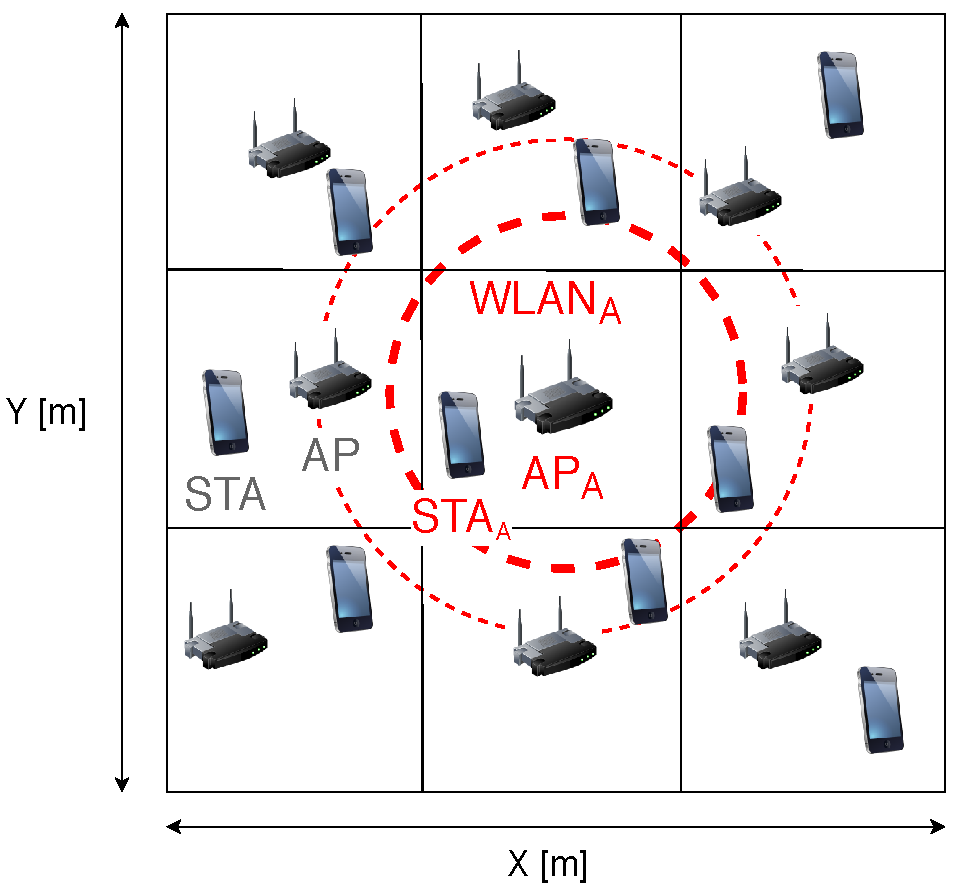
\epsfig{file=random_scenario.pdf, width=5.5cm}
		\caption{Random grid scenario containing 9 WLANs. The location of $\text{WLAN}_A$ is fixed to the center.}
		\label{fig:random_scenario}
	\end{figure}

    The simulation parameters are provided in Table \ref{table:parameters}. The scenario is divided into 9 cells, but the location of $\text{WLAN}_A$ is always fixed in the center of the scenario. For the rest of the APs and STAs, their position is randomly selected within their corresponding cell. The configuration of each WLAN is set homogeneously: they all use the same channel, the default sensitivity is set to -82 dBm, and the default transmission power is set to 20 dBm. Notice that, for dense deployments, $\text{WLAN}_A$ is expected to suffer a higher level of interference than the others, which allows us to assess the effectiveness of the SR operation in crowded environments.

	\begin{table}[h]
		\centering
		\resizebox{\columnwidth}{!}{
			\begin{tabular}{c|l|l|}
				\cline{2-3}
				\multicolumn{1}{l|}{} & \textbf{Parameter} & \textbf{Value}
				\\ \hline
				% PHY
				\multicolumn{1}{|c|}{\multirow{9}{*}{\rotatebox[origin=c]{90}{PHY}}} & Central frequency, $f_c$ & 5 GHz \\ \cline{2-3} 
				\multicolumn{1}{|c|}{} & Transmission gain, $G_{tx}$ & 0 dB \\ \cline{2-3} 
				\multicolumn{1}{|c|}{} & Reception gain, $G_{rx}$ & 0 dB \\ \cline{2-3} 
				\multicolumn{1}{|c|}{} & Path-loss (residential scenario), $\text{PL}(d)$ & See \cite{pathloss11ax}  \\ \cline{2-3}
				\multicolumn{1}{|c|}{} & Background noise level, $N$ & -95 dBm \\ \cline{2-3}
				\multicolumn{1}{|c|}{} & Legacy OFDM symbol duration, $\sigma_\text{leg}$ & 4 \textmu s \\
				\cline{2-3}
				\multicolumn{1}{|c|}{} & OFDM symbol duration (GI-32), $\sigma$ & 16 \textmu s \\ 				\cline{2-3}
				\multicolumn{1}{|c|}{} & Number of subcarriers (20 MHz), $N_{sc}$ & 234   \\
				\cline{2-3}
				\multicolumn{1}{|c|}{} & Number of spatial streams, $N_{ss}$ & 1  \\
				\cline{2-3}
				\multicolumn{1}{|c|}{} & Transmit power levels, $\mathcal{T}$ & 1 to 20 dBm (1 dBm steps) \\
				\hline
				% MAC
				\multicolumn{1}{|c|}{\multirow{16}{*}{\rotatebox[origin=c]{90}{MAC}}} & Empty slot duration, $\text{T}_e$ & 9 $\mu$s\\ 
				\cline{2-3} 
				\multicolumn{1}{|c|}{} & SIFS duration, $T_\text{SIFS}$ & 16 \textmu s  \\
				\cline{2-3} 
				\multicolumn{1}{|c|}{} & DIFS/AIFS duration, $T_\text{DIFS/AIFS}$ & 34 \textmu s \\
				\cline{2-3} 
				\multicolumn{1}{|c|}{} & PIFS duration, $T_\text{PIFS}$  & 25 \textmu s \\
				\cline{2-3} 
				\multicolumn{1}{|c|}{} & Legacy preamble duration, $T_\text{PHY-leg}$ & 20 \textmu s  \\
				\cline{2-3}
				\multicolumn{1}{|c|}{} & HE single-user field duration, $T_\text{HE-SU}$ & 100 \textmu s \\
				\cline{2-3} 
				\multicolumn{1}{|c|}{} & ACK duration, $T_\text{ACK}$ & 28 \textmu s\\
				\cline{2-3} 
				\multicolumn{1}{|c|}{} & Block ACK duration, $T_\text{BACK}$ & 32 \textmu s \\
				\cline{2-3} 
				\multicolumn{1}{|c|}{} &  Size OFDM symbol (legacy), $L_{s,l}$ & 24 bits \\
				\cline{2-3} 
				\multicolumn{1}{|c|}{} & Length of data packets, $\text{L}_{d}$ & 12,000 bits \\
				\cline{2-3} 
				\multicolumn{1}{|c|}{} & No. of frames in an A-MPDU, $N_{\text{agg}}$ & 64 \\
				\cline{2-3} 
				\multicolumn{1}{|c|}{} & Length of an RTS packet, $L_\text{RTS}$ & 160 bits \\
				\cline{2-3} 
				\multicolumn{1}{|c|}{} & Length of a CTS packet, $L_\text{CTS}$ & 112 bits \\
				\cline{2-3} 
				\multicolumn{1}{|c|}{} & Length of service field, $L_\text{SF}$ & 16 bits  \\
				\cline{2-3} 
				\multicolumn{1}{|c|}{} & Length of MAC header, $L_\text{MH}$ & 320 bits \\
				\cline{2-3} 
				\multicolumn{1}{|c|}{} & Contention window (fixed), $\text{CW}$ & 15 \\
				\cline{2-3} 
				\multicolumn{1}{|c|}{} & Allowed sensitivity levels, $\mathcal{S}$ & -82 to -62 (1 dBm steps) \\
				\hline
				% Other
		    	\multicolumn{1}{|c|}{\multirow{2}{*}{\centering\rotatebox[origin=c]{90}{Misc.  }}} & Traffic model, $\Lambda$ & Downlink (UDP)\\
				\cline{2-3} 
				\multicolumn{1}{|c|}{} & Traffic generation ratio, $l$ & 1,000, 2,000 and 10,000 pkts/s\\ 
				\cline{2-3} 
				\multicolumn{1}{|c|}{} & Map area (random scenario), $A$ & 625, 400, 225 and 100 m$^2$\\
				\hline
		\end{tabular}}
		\caption{Simulation parameters.}
		\label{table:parameters}
	\end{table}
	
	%%% DENSITY
	\subsection{Network Density}
	\label{section:random_scenarios_density}
    In order to capture the effects of using SR according to network density, we consider four different map sizes: sparse ($25\times25$ m), semi-dense ($20\times20$ m), dense ($15\times15$ m) and ultra-dense ($10\times10$ m). For each type of scenario, we provide 50 different deployments, in which APs and STAs are placed uniformly at random within their corresponding cell. $\text{WLAN}_A$ is the only one applying the SR operation. Therefore, since we compute all the possible OBSS/PD values to be used by $\text{WLAN}_A$, in total we have $21\times4\times50 = 4200$ scenarios.
	
	Fig. \ref{fig:SIM_2_1} shows the average throughput achieved by default and when applying the SR operation in $\text{WLAN}_A$. In particular, we differentiate between the individual throughput of $\text{WLAN}_A$ and the average throughput of the other WLANs. For each network density, we have tried all the possible OBSS/PD values to be used by $\text{WLAN}_A$. Then, we have chosen the best possible result and compare it with the results obtained when using the default CCA/CS.
	
	\begin{figure}[ht!]
		\centering		
		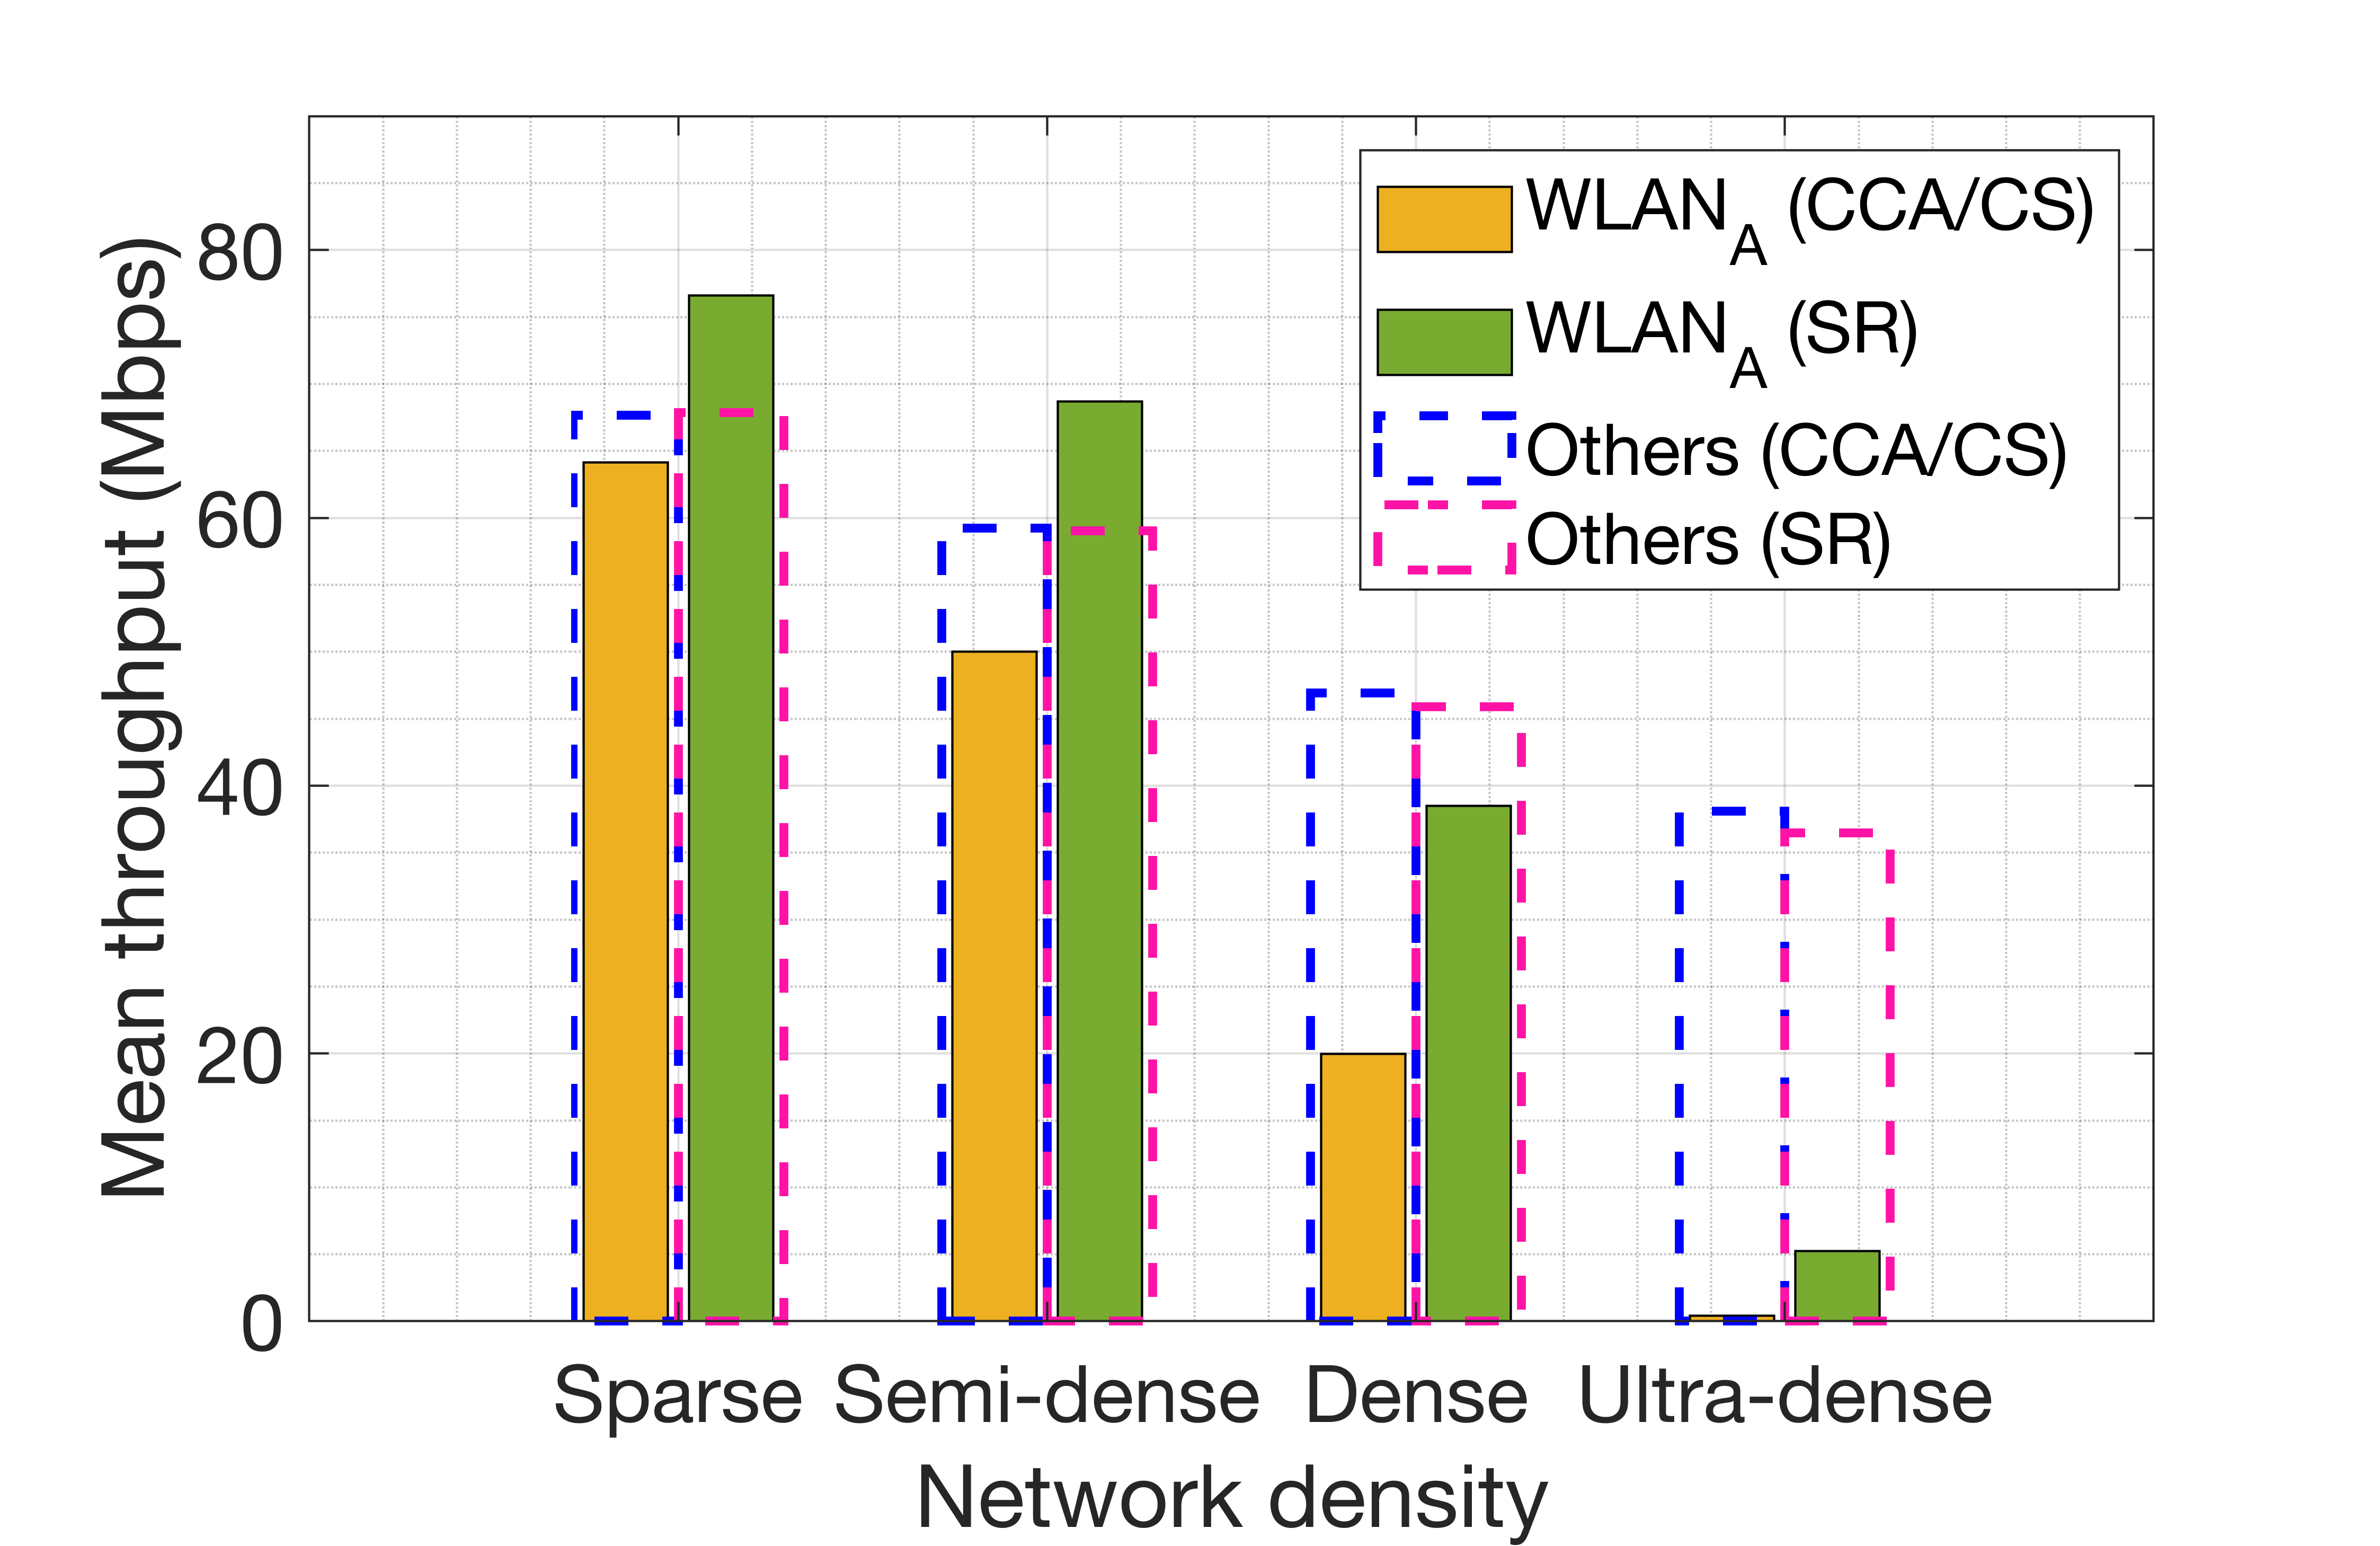
\includegraphics[width=\columnwidth]{SIM_2_1}
		\caption{Mean throughput achieved with and without applying the SR operation in $\text{WLAN}_A$, for each network density. Results show the mean throughput achieved by $\text{WLAN}_A$ and the rest of WLANs.}
		\label{fig:SIM_2_1}
	\end{figure}
	
	First of all, if we focus on the throughput that $\text{WLAN}_A$ experiences by default (amber solid bars), we notice a dramatic decrease as network density increases. Nevertheless, the SR operation allows to significantly overcome the high levels of channel contention noticed by $\text{WLAN}_A$ (displayed by the green solid bars). Note, as well, that the maximum improvement is experienced for the dense scenario ($15\times15$ m). While the default performance is quite high for sparser scenarios, the ultra-dense scenario supposes a barrier to keep improving the performance (the level of interference is that high that channel reutilization cannot be further improved).
	
	Apart from that, we observe that the average performance of the other WLANs (dashed bars) does not suffer radical changes for any of the network densities when $\text{WLAN}_A$ applies SR. This is a really positive result, which indicates that the SR operation allows maximizing the individual performance without affecting the environment (i.e., legacy devices that do not apply the operation).
	
	%%% TRAFFIC LOAD
	\subsection{Traffic load}
	\label{section:random_scenarios_traffic_load}
	In addition to network density, the traffic load is another key factor to be studied with regards to the SR operation. To that purpose, we focus on the second densest scenario, which has been previously shown to achieve the maximum gains of the SR operation. In particular, we provide three different traffic loads ($l$), which are the same for all the WLANs: \emph{i)} low (1,000 packets/s, i.e., 12 Mbps), \emph{ii)} medium (2,000 packets/s, i.e., 24 Mbps), and \emph{iii)} high (10,000 packets/s, i.e., 120 Mbps). The traffic type considered is UDP in the downlink, which injects packets to the AP's queue following a Poisson distribution with $\lambda$ equal to the traffic load considered in each case.
		
	Fig. \ref{fig:SIM_2_2} compares the performance achieved by using the default CCA/CS and by applying the SR operation. As done before, results target the individual performance of $\text{WLAN}_A$ and the average performance of the other WLANs. In particular, Fig. \ref{fig:SIM_2_2_2} shows the maximum improvements achieved by WLAN$_A$ in terms of throughput. Notice that the SR configuration considers the OBSS/PD values that maximize WLAN$_A$'s throughput. Based on that configuration, Fig. \ref{fig:SIM_2_2_1} shows the average channel occupancy (in \%).
	
	\begin{figure}[ht!]
		\centering		
		%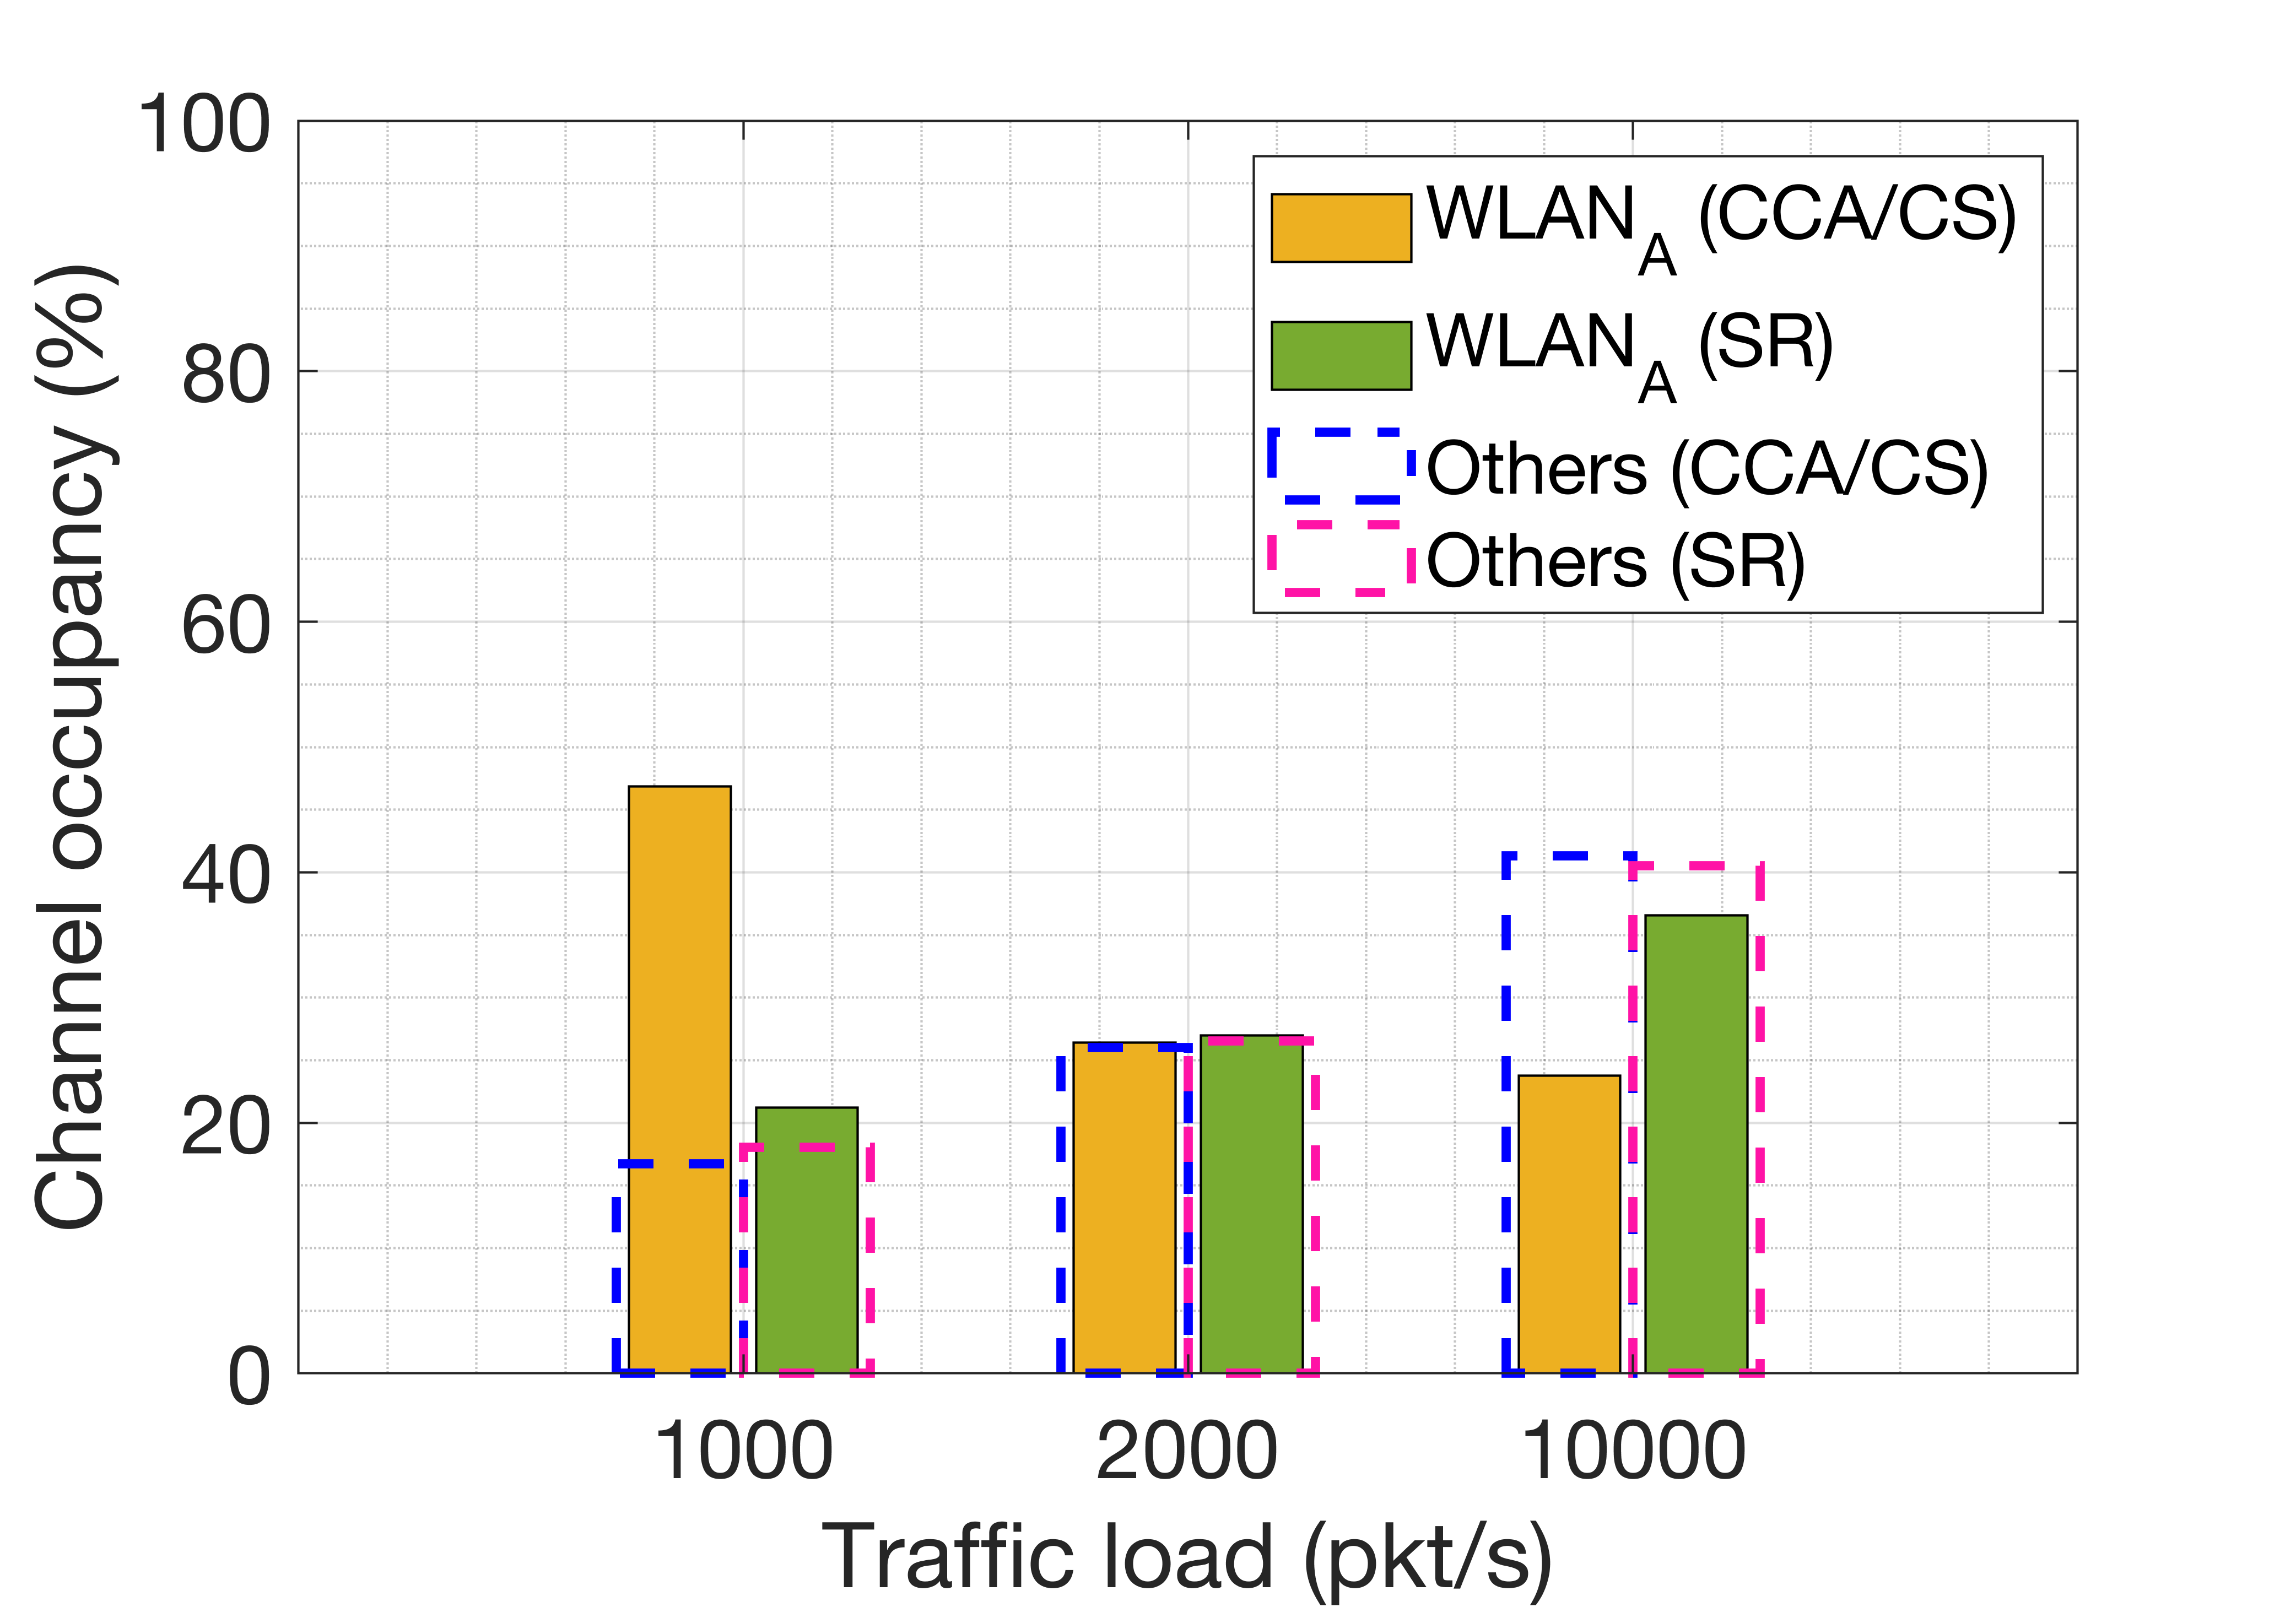
\includegraphics[width=\columnwidth]{SIM_2_2_1}
		\subfigure[Throughput]{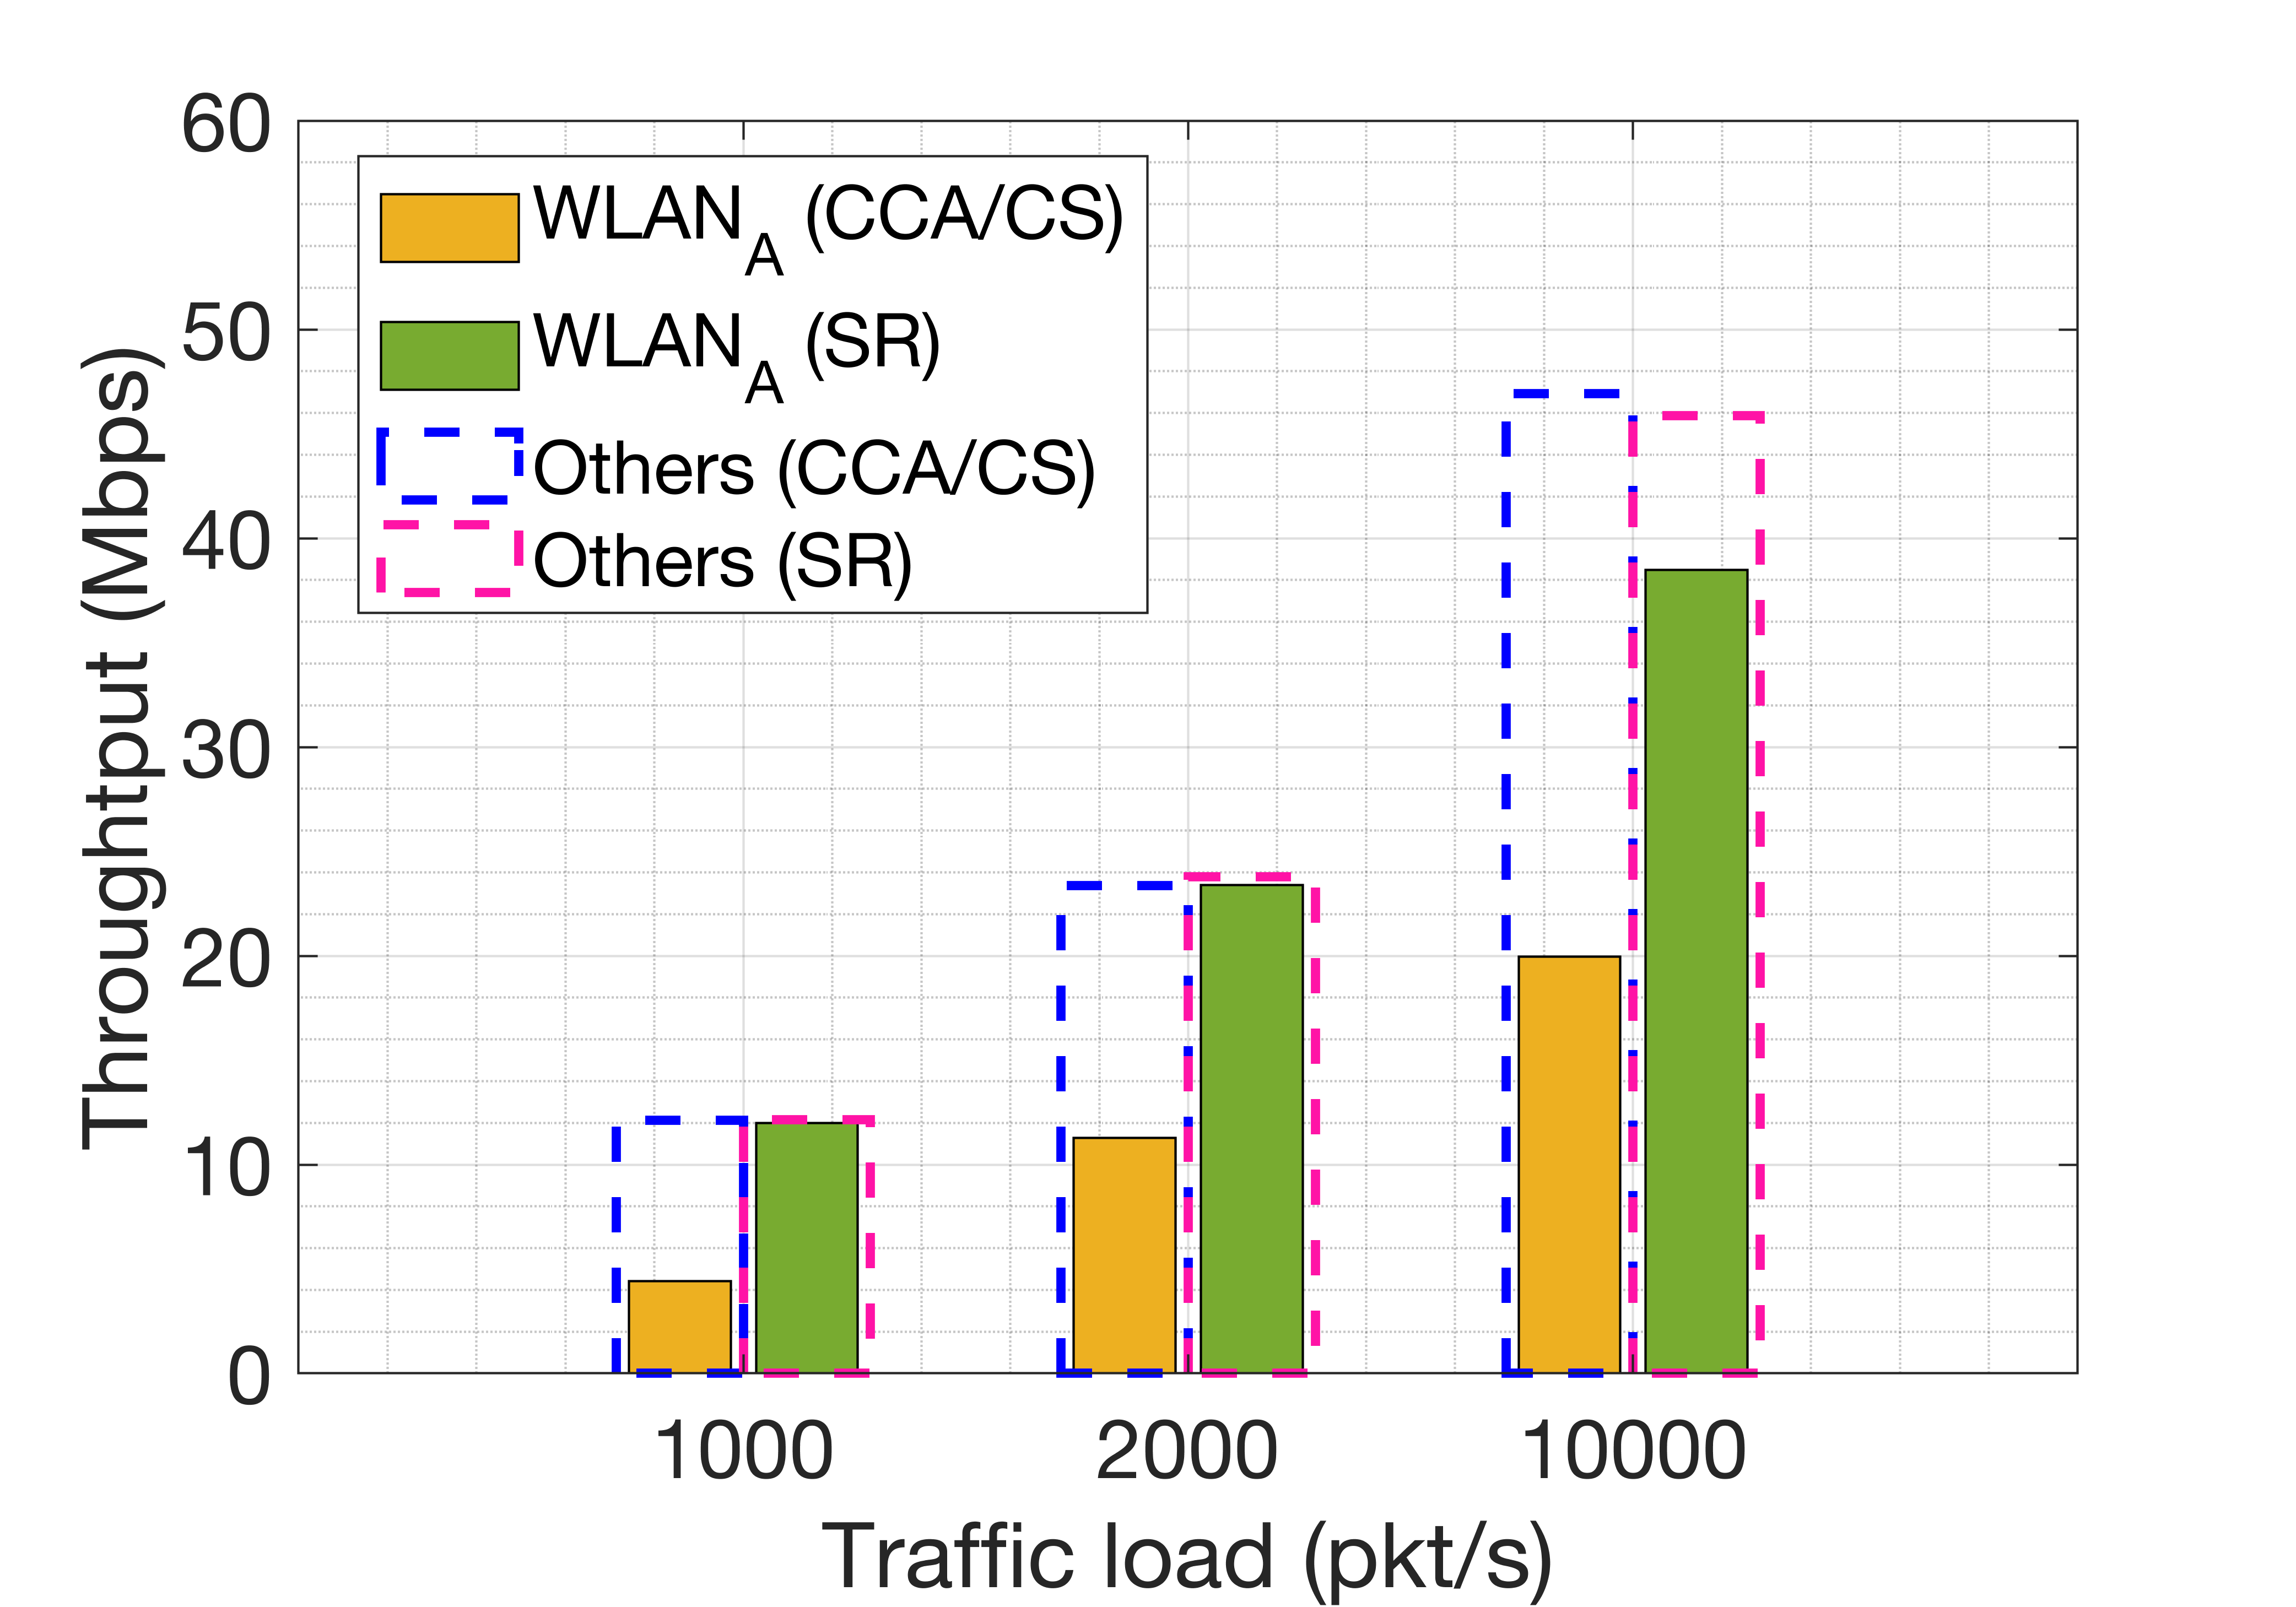
\includegraphics[width=\columnwidth]{SIM_2_2_2}\label{fig:SIM_2_2_2}}
		\subfigure[Traffic load]{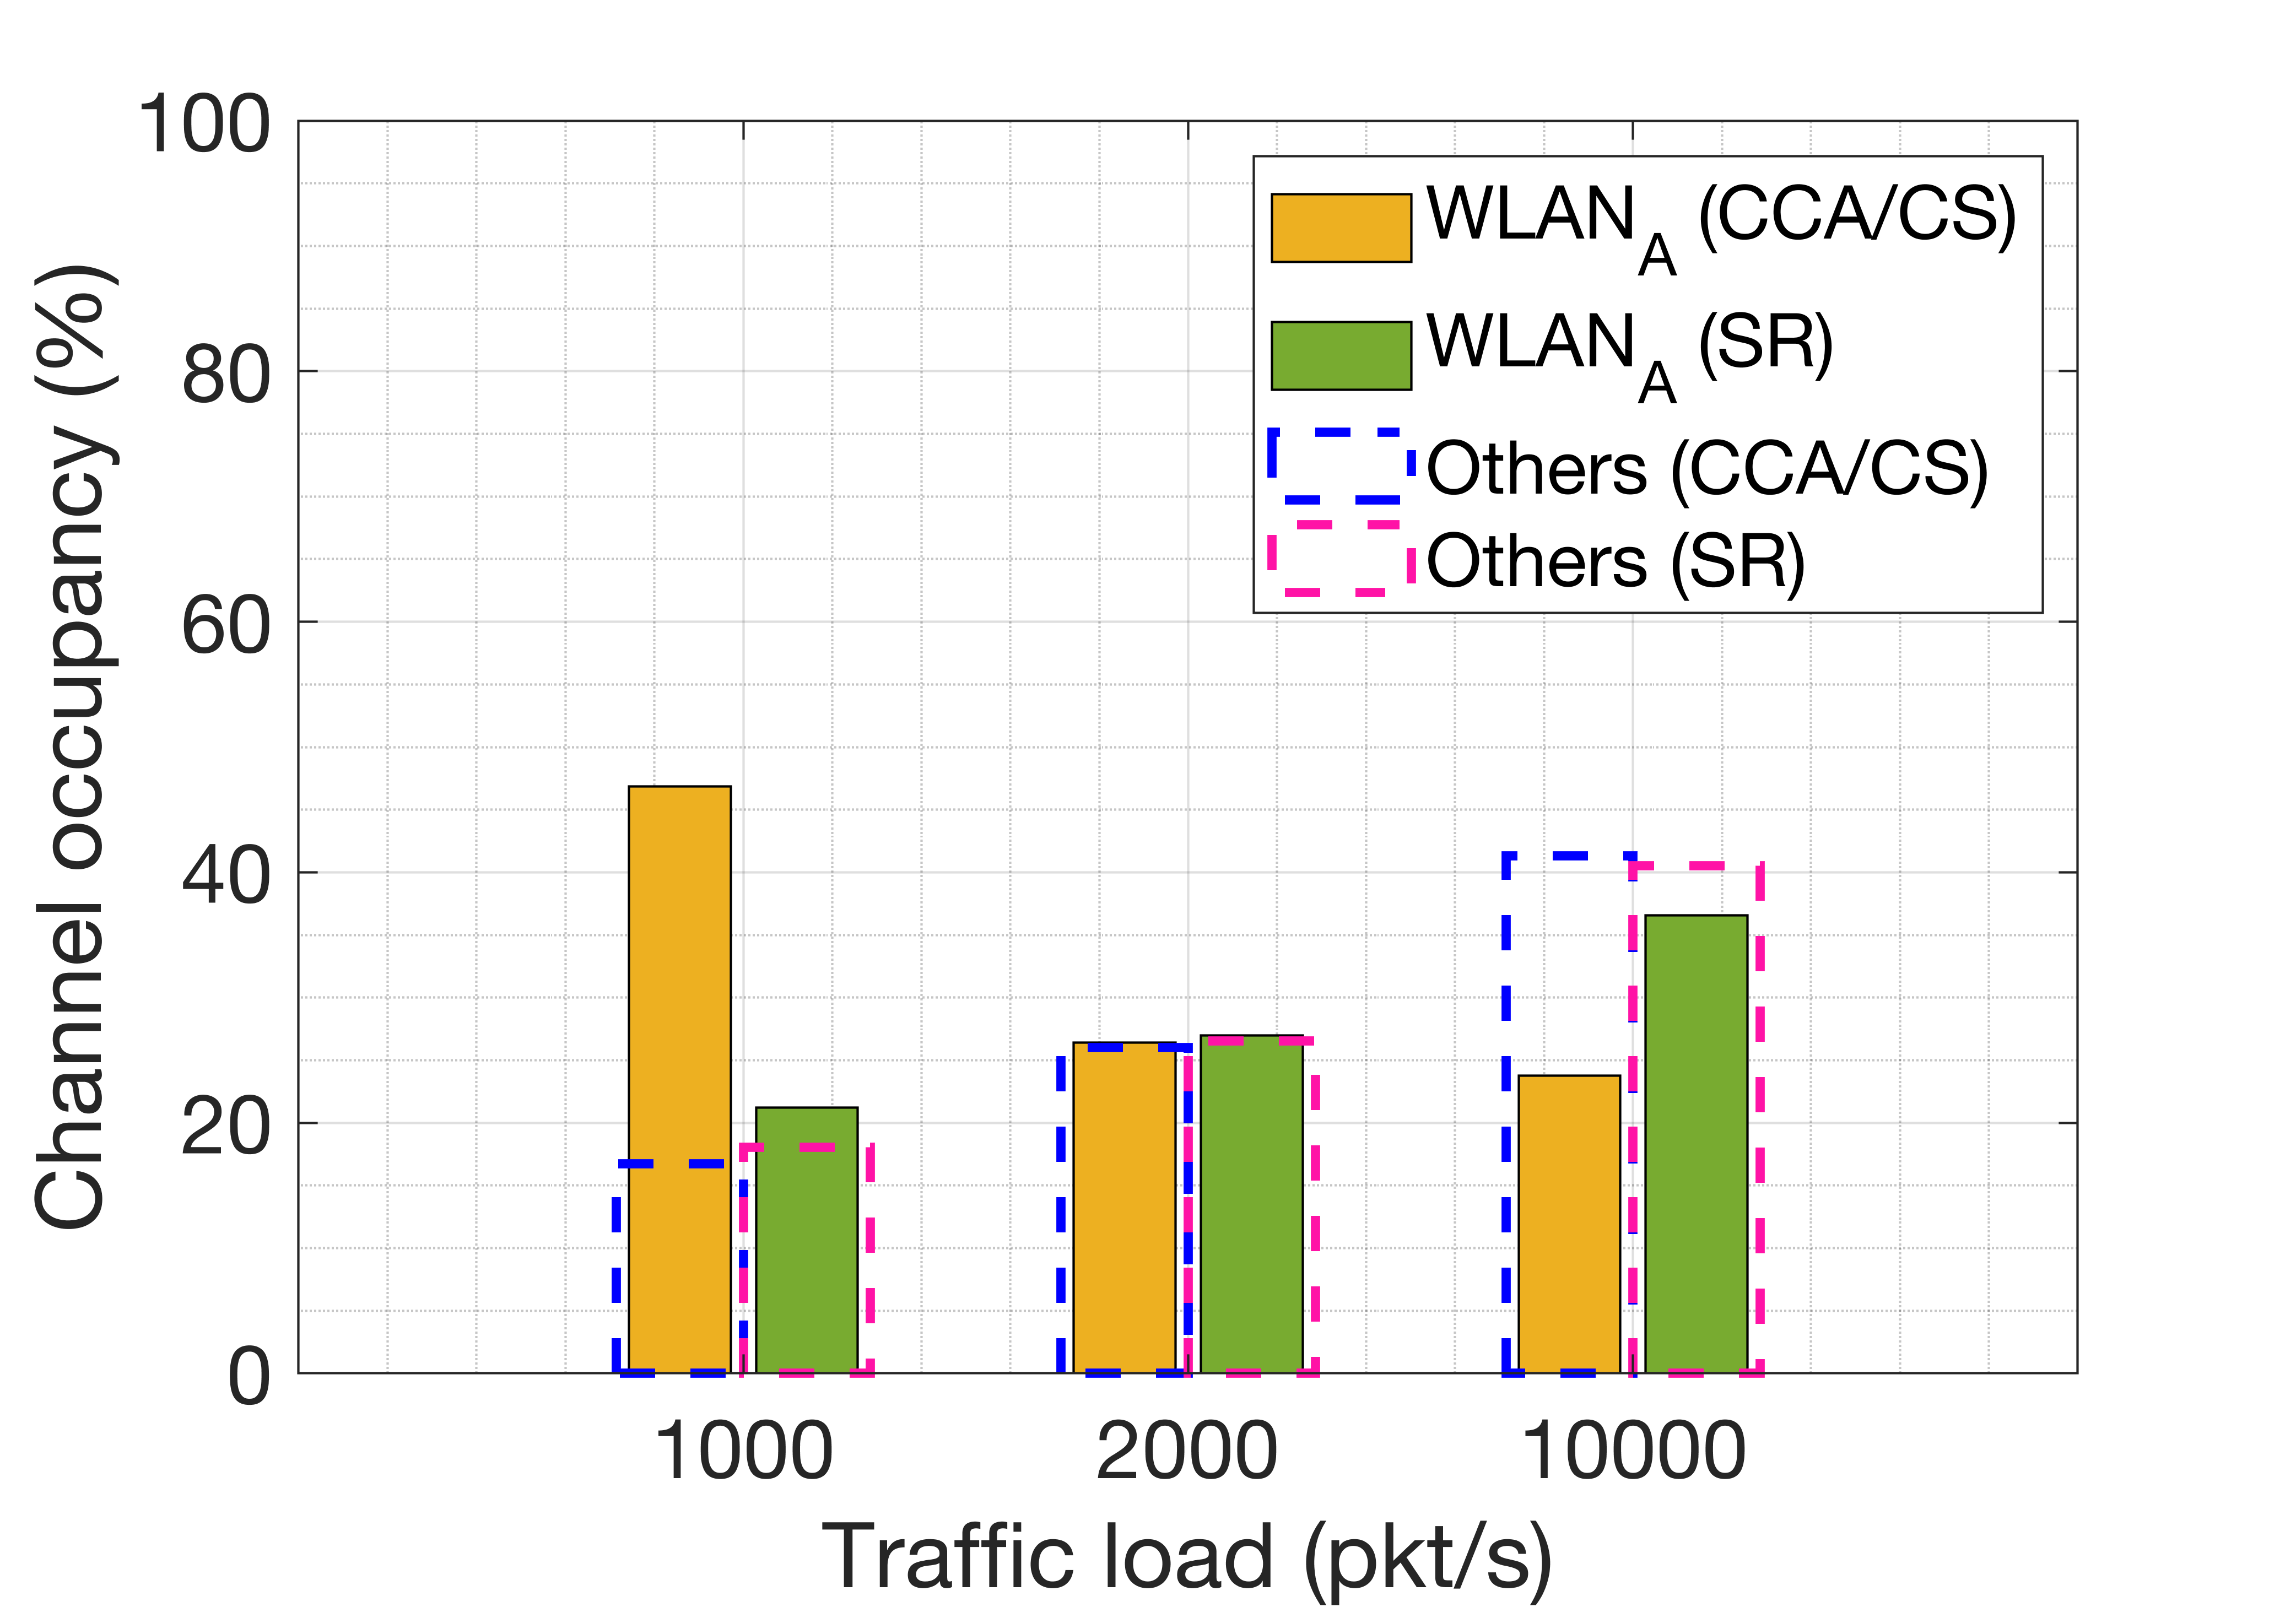
\includegraphics[width=\columnwidth]{SIM_2_2_1}\label{fig:SIM_2_2_1}}
		\caption{Mean performance achieved with and without applying the SR operation in $\text{WLAN}_A$, for each traffic load. Results are shown for $\text{WLAN}_A$ and for the rest of WLANs (others).}
		\label{fig:SIM_2_2}
	\end{figure}
	
	As shown in Fig. \ref{fig:SIM_2_2_2}, greater improvements on the throughput of $\text{WLAN}_A$ are achieved as traffic load increases. In particular, the greatest gain is noticed for the largest traffic load (10,000 packets/s), which entails a saturation regime. This is a quite remarkable result since the interference noticed by $\text{WLAN}_A$ is much higher when all the surrounding devices are constantly transmitting due to their high traffic load. Regarding channel occupation (shown in Fig. \ref{fig:SIM_2_2_1}), an interesting phenomenon is observed for the lowest traffic load. The fact is that the legacy CCA/CS configuration provides a higher channel occupancy than the SR one. However, this is not translated into higher throughput, due to the high number of experienced collisions. Notice that those collisions entail a high number of re-transmissions, which cause such an increase in the occupancy.
	
	Finally, it is worth pointing out that the performance of the other WLANs is not affected in case $\text{WLAN}_A$ applies SR.
	
	%%% COLLABORATIVE SR
	\subsection{Joint Spatial Reuse Operation}
	\label{section:random_scenarios_collaborative}
	So far, we have studied the effects of applying SR in a single WLAN (i.e., $\text{WLAN}_A$). Now, we assess the potential of the joint operation by defining different situations according to the number of WLANs that apply SR. Provided that $\text{WLAN}_A$ always applies the SR operation, we propose three cases: 
	\begin{itemize}
		\item \textbf{Legacy:} all the other WLANs employ the default CCA/CS.
		\item \textbf{Mixed SR:} at the beginning of the simulation, each WLAN randomly decides (with same probability) whether to apply the SR operation or to remain using the default configuration.
		\item \textbf{All SR:} all the WLANs apply the SR operation. 
	\end{itemize}
	
	In order to compare the effects of applying SR in parallel with other WLANs, we define the following metrics: \emph{i)} throughput ($\Gamma$), \emph{ii)} percentage of time occupying the channel ($\rho$), and \emph{iii)} average delay for transmitting a packet once it arrives at the queue ($d$). For each metric, we consider the performance improvements achieved by $\text{WLAN}_A$ (indicated with subindex \emph{A}), and the average across the rest of WLANs (indicated with subindex \emph{O}).

	Fig. \ref{fig:SIM_2_3} shows the potential improvements achieved when applying SR in every type of scenario. While Fig. \ref{fig:SIM_2_3_1} shows the performance of WLAN$_A$, Fig. \ref{fig:SIM_2_3_2} focuses on the performance of the others. For that purpose, the empirical cumulative distribution function (CDF) is used for each of the performance metrics. Notice that we have considered the densest scenario ($25\times25$m) and the highest traffic load (10,000 packets/s), thus representing a worst-case situation. As done before, we have generated 50 random scenarios for averaging purposes, and, for each of them, we have tried all the possible OBSS/PD values to be used homogeneously by the WLANs applying the SR operation. Accordingly, we have used the best value to extract the maximum average improvement of SR with respect to the legacy configuration. In every situation (\emph{legacy}, \emph{mixed} and \emph{all SR}), we pick the best OBSS/PD threshold from $\text{WLAN}_A$'s point of view, which is also used to assess its impact on the others. Again, the SR configuration used for the channel occupancy is the one that maximizes $\text{WLAN}_A$'s throughput.
	
	\begin{figure}[ht!]
		\centering		
		\subfigure[WLAN$_A$]{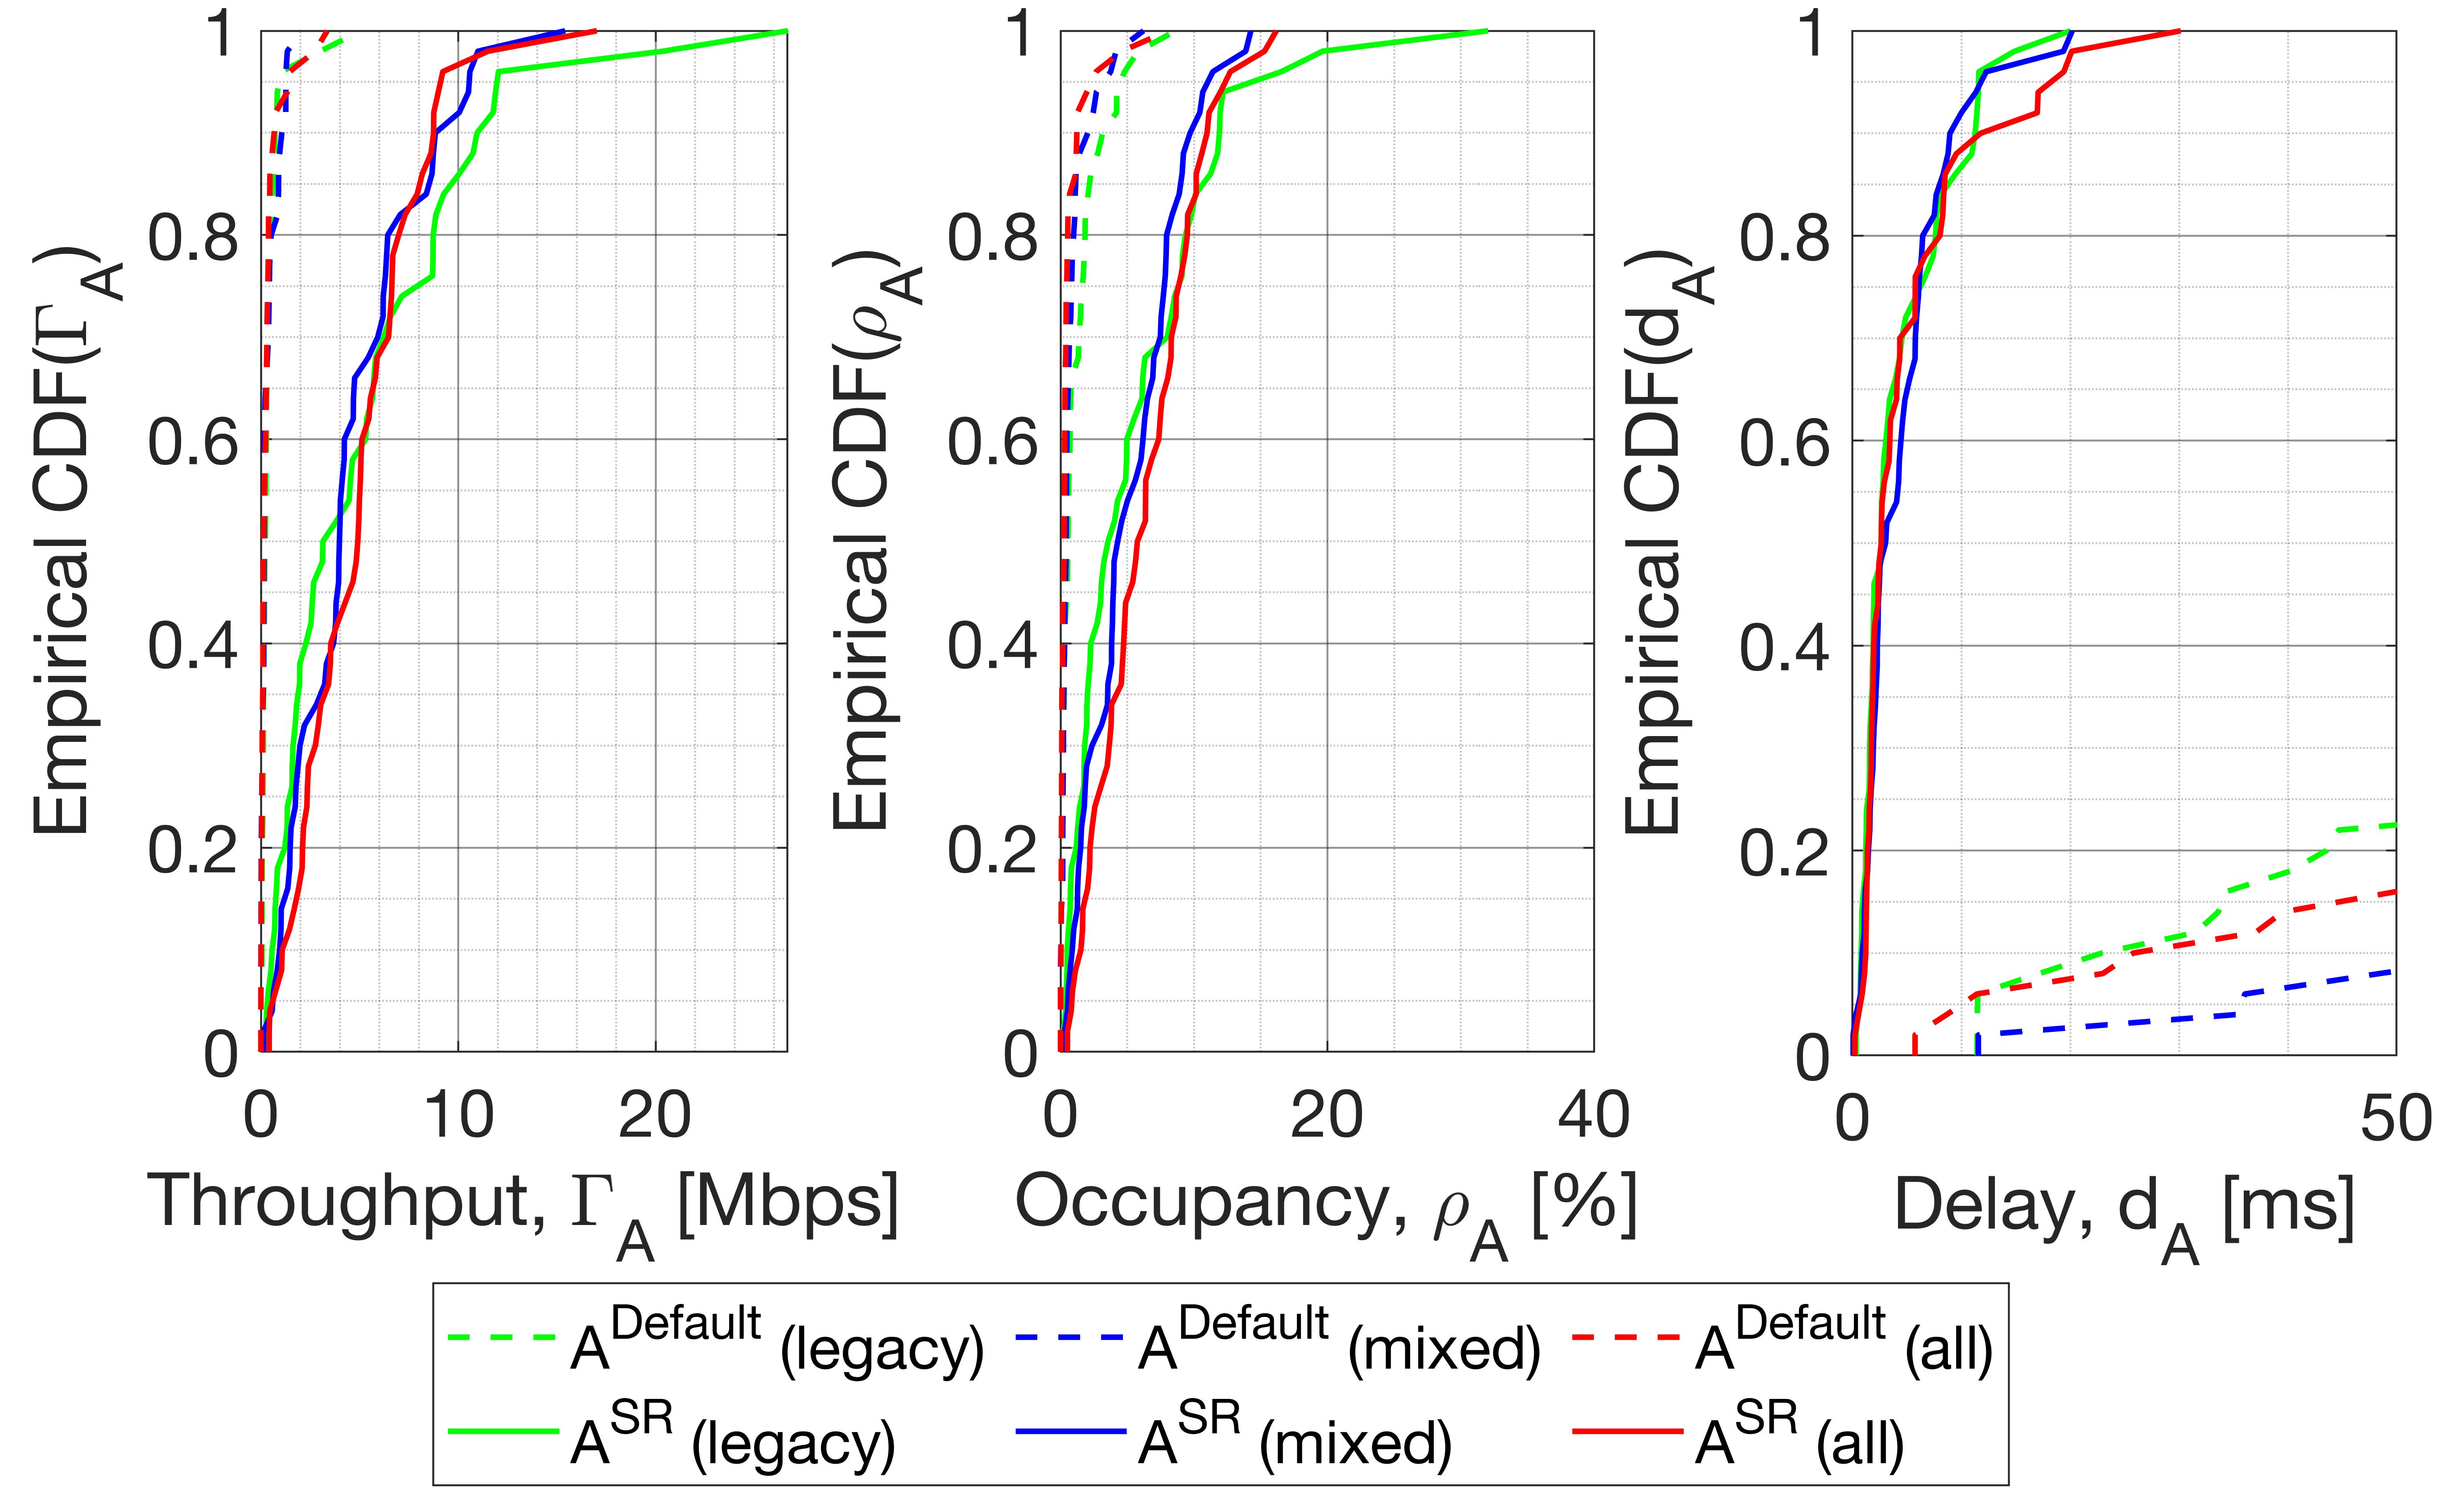
\includegraphics[width=\columnwidth]{SIM_2_3_1}\label{fig:SIM_2_3_1}}
		\subfigure[Others]{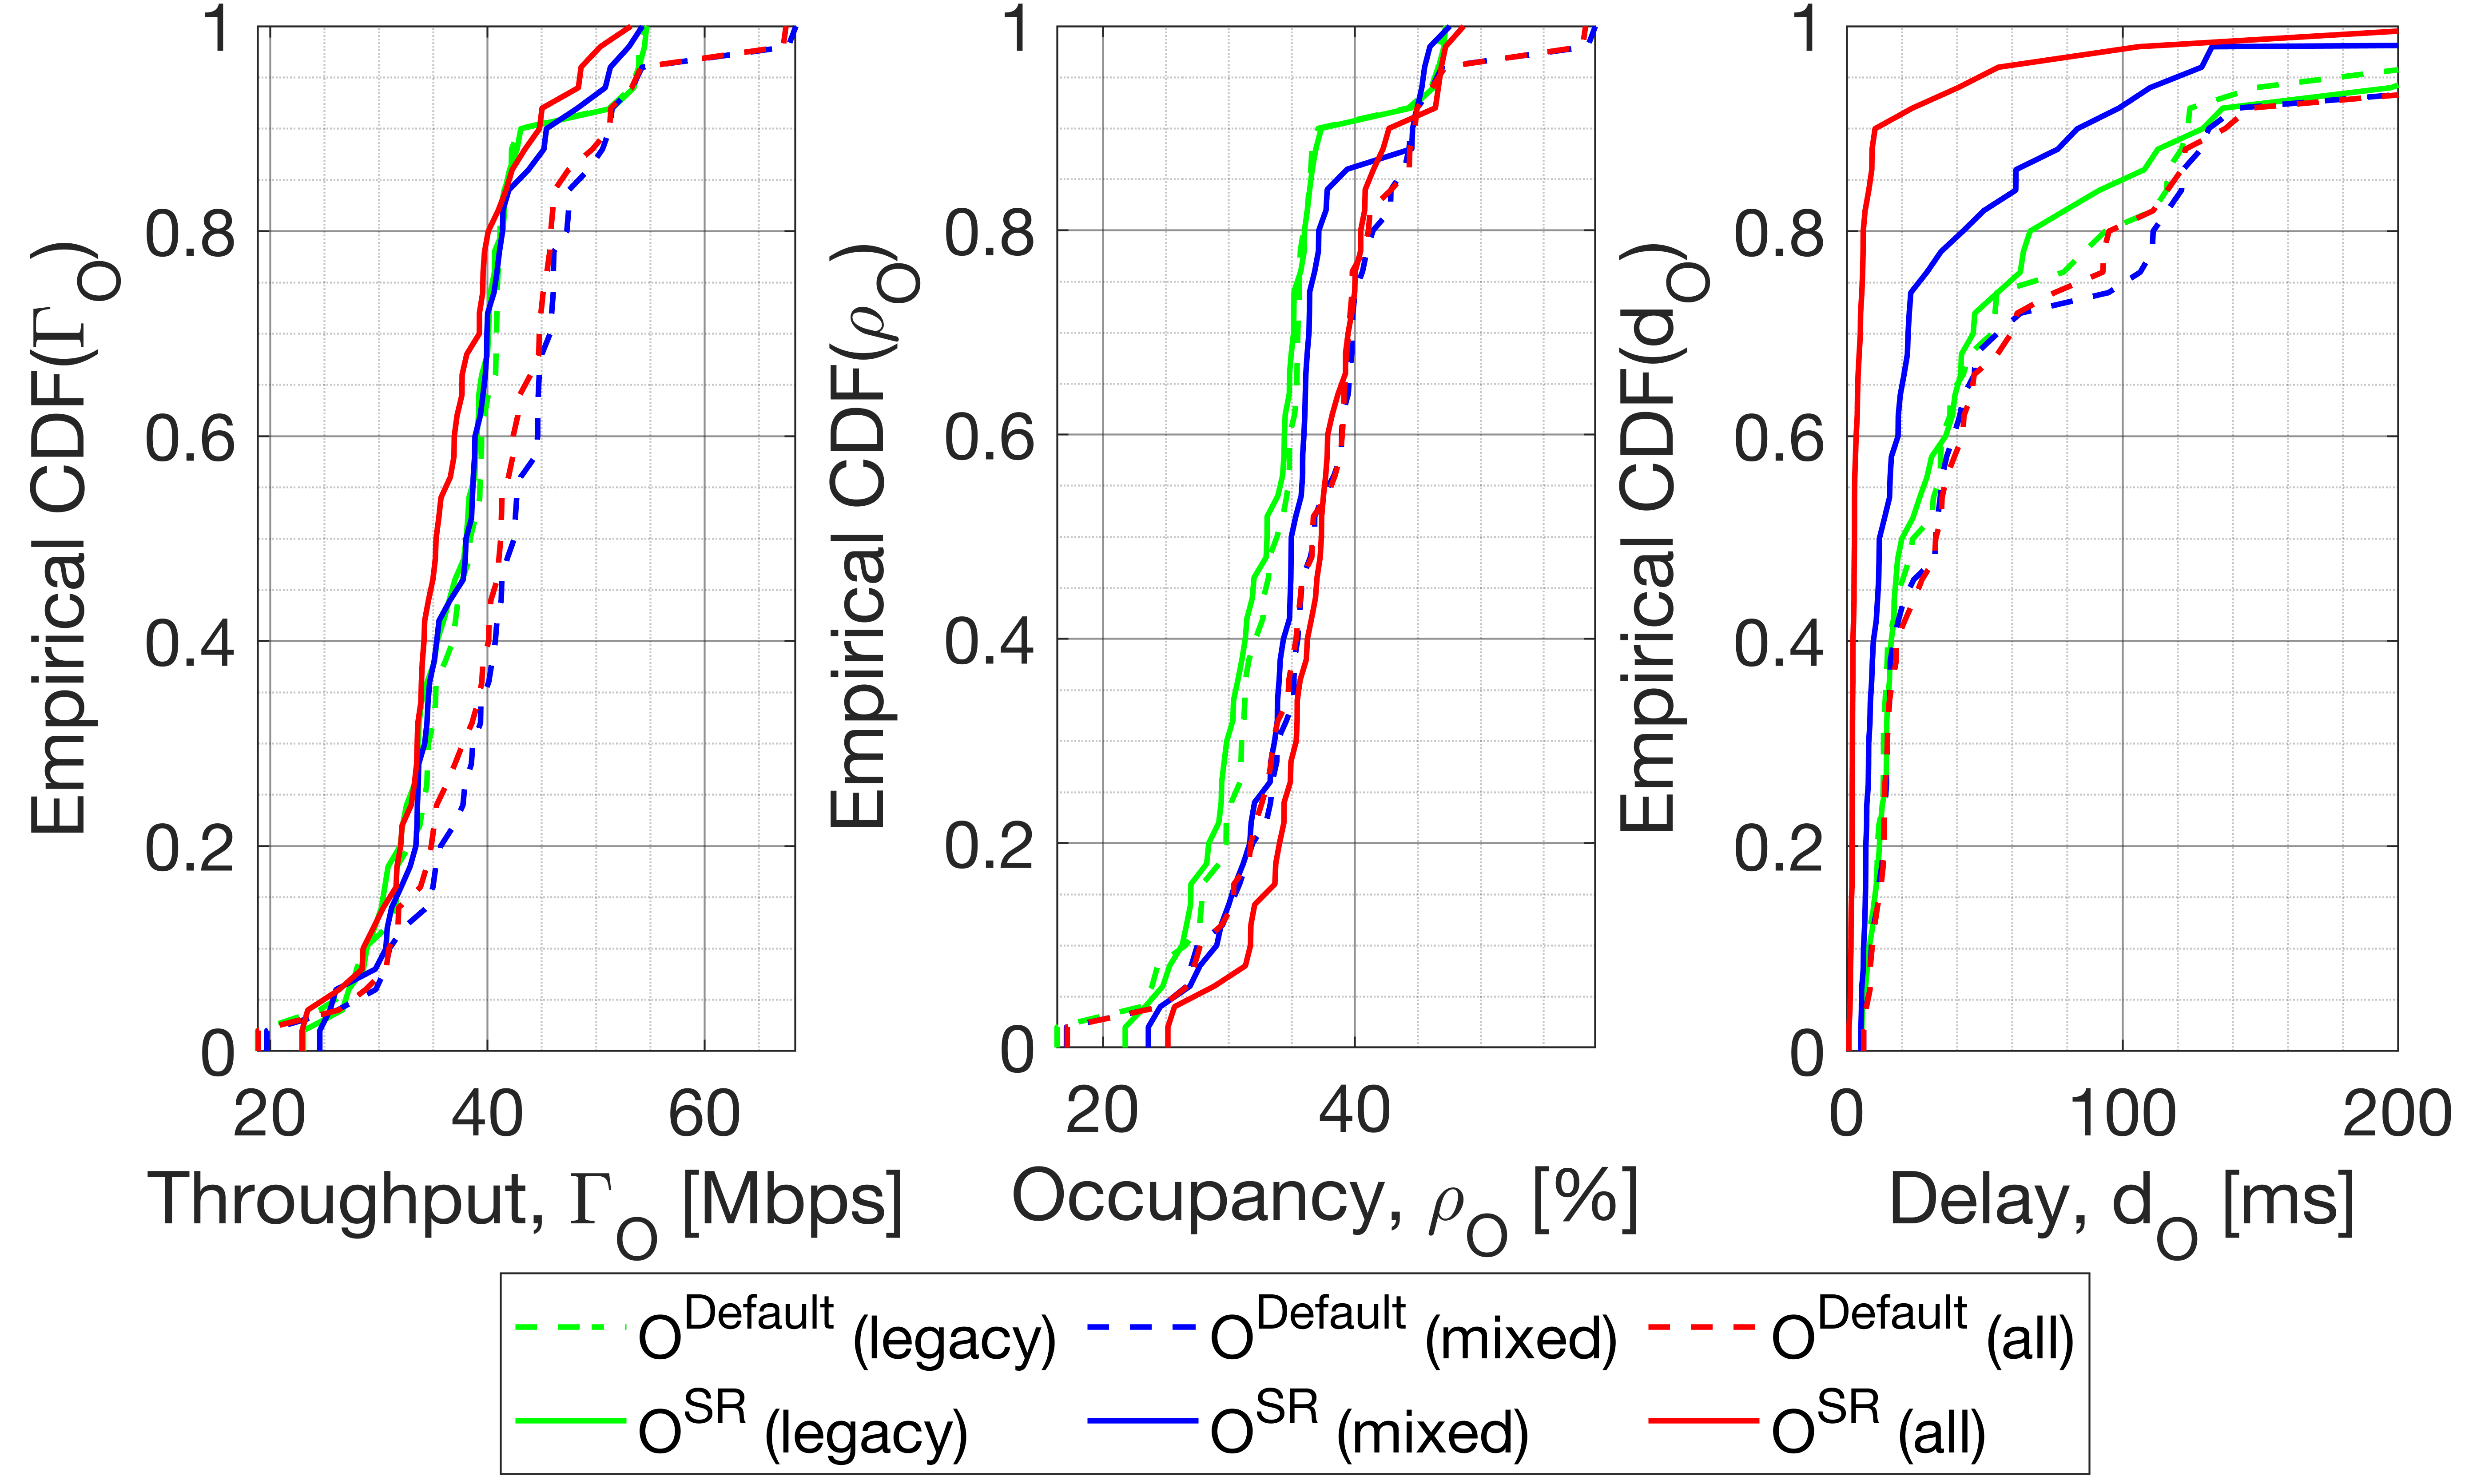
\includegraphics[width=\columnwidth]{SIM_2_3_2}\label{fig:SIM_2_3_2}}
		\caption{Mean performance improvements achieved for each SR setting by WLAN$_A$ ($A$) and the others ($O$). The results are shown for the OBSS/PD values that maximize the performance of WLAN$_A$.}\label{fig:SIM_2_3}
	\end{figure}
	
	As shown in Fig. \ref{fig:SIM_2_3_1}, $\text{WLAN}_A$ achieves similar performance improvements, regardless of whether the environment applies SR or not. In particular, a high gain is noticed on the average delay. Moreover, regarding the others' performance (Fig. \ref{fig:SIM_2_3_2}), a null improvement is observed on the throughput, even for the \emph{all SR} context. In contrast, the delay is notably reduced as the number of WLANs using SR increases.
	
	% ----------------------------------
	% -
	% 	-- Gaps --
	% -
	% ----------------------------------
	\section{Ways Forward and Research Opportunities}
	\label{section:ways_forwad}
	The IEEE 802.11ax SR operation can potentially increase spectral efficiency in dense deployments. However, there are several blind spots that must be overcome in order to sustain progress towards next-generation wireless deployments. 
	
	\subsection{Unexplored Areas within the Spatial Reuse Operation}
	In particular, the following areas in the context of the SR operation have not been fully exploited yet:
	\begin{itemize}
		\item \textbf{Assignment of BSS colors:} as discussed in Sections \ref{section:bss_coloring} and \ref{section:obss_pd_based}, BSS coloring is key for the OBSS/PD-based SR operation since it allows differentiating between intra and inter-BSS frames. However, the way BSS colors are assigned to WLANs is not specified, thus leading to potential collisions and miss-behaviors regarding the SR operation.
		\item \textbf{Election of SRGs:} similarly to the BSS color, the SRG is used to sub-classify inter-BSS frames, so that different PD policies can be applied to increase spectral efficiency. However, forming SRGs is not trivial, since inter-WLAN interactions must be carefully captured to properly taking advantage of the SR operation. The set of policies regarding SRGs may be decided by the APs, as a result of a previous information gathering (e.g., after experiencing several packet losses for the default configuration).
		\item \textbf{Establishment of PD thresholds:} the election of PD thresholds for each type of frame (SRG, and non-SRG) must be carefully done. On the one hand, too low values may lead to null improvement, thus framing the legacy operation whereby the channel is shared. On the other hand, too high values may generate performance anomalies such as the hidden-terminal problem or flow starvation. In order to properly establish each PD threshold, all the possible interactions between WLANs must be captured on a per-STA basis.
		\item \textbf{Optimal transmit power:} the current transmit power restriction is useful to prevent the accentuation of unfair situations. However, the performance of the SR operation may be further increased in case of properly leveraging the transmit power according to the noticed interactions among nodes.
		\item \textbf{Disabling the SR operation:} there are situations in which the SR operation may be harmful to certain devices (e.g., in terms of fairness). Therefore, a given WLAN must be able to identify whether the SR operation must be disabled or not. This can be achieved by setting the OBSS/PD threshold to the default CCA/CS value. Alternatively, the SR operation can be disabled at STAs only, thus leading to an AP-only SR setting. In this regard, AP-AP interactions would be mostly targeted.
	\end{itemize}
	
	Solving most of the aforementioned problems is not straightforward and requires an in-depth analysis to offer optimal or close-to-optimal solutions. While BSS color assignment may appear to be straightforward (e.g., through graph coloring techniques), defining PD thresholds is a very complex task that embraces many variables. In particular, inter-WLAN interactions have been shown in this paper to significantly vary depending on the chosen OBSS/PD. Since the performance of IEEE 802.11 WLANs is not linear with the sensitivity and the transmission power (due to the nature of CSMA/CA), the optimal PD threshold cannot be computed explicitly. 
	
	Notice that the number of total combinations in an N-WLANs scenario is $C = 21^\text{N}$, provided that only intra and inter-BSS frames are differentiated and that 21 possible OBSS/PD thresholds are allowed. Therefore, the problem is intractable. Moreover, when considering SRGs, the problem becomes even more complex. In that case, the number of combinations is $C = (21\times21)^\text{N}$, provided that we have 21 values to be used for each PD threshold type (SRG OBSS/PD, and non-SRG OBSS/PD).
	
	\subsection{Integration of the Spatial Reuse Operation with other Techniques}
	
	% Other ways forward
	In addition to problems specific to the SR operation, the integration with many other novel mechanisms is unexplored. Among them, we highlight OFDMA \cite{bankov2018ofdma, dovelos2018optimal}, multiple antenna systems \cite{liao2016mu}, and scheduled transmissions \cite{nurchis2019target}. The potential of the 11ax SR operation goes further when combined with other techniques. 
	
	For instance, the combination of SR with directional transmissions may lead to efficient and performance maximizing communications, where SR is applied on a per-beam basis. Fig. \ref{fig:sr_and_beamforming} devises the potential of combining SR with directional transmissions. As illustrated, $\text{WLAN}_A$ applies the SR operation on a per-beam basis, while $\text{WLAN}_B$ remains using the default CCA/CS. In particular, collisions by hidden-node may be experienced for $\text{STA}_\text{A3}$, in case of using the inter-BSS OBSS/PD. However, channel reuse can be enhanced for transmissions to $\text{STA}_\text{A1}$ and $\text{STA}_\text{A2}$, which are out of range of $\text{AP}_B$. Therefore, the inter-BSS OBSS/PD can be used only for transmissions involving those two STAs, while a more conservative threshold (i.e., the legacy CCA/CS) can be employed for $\text{STA}_\text{A3}$.
	
	\begin{figure}[ht!]
		\centering		
		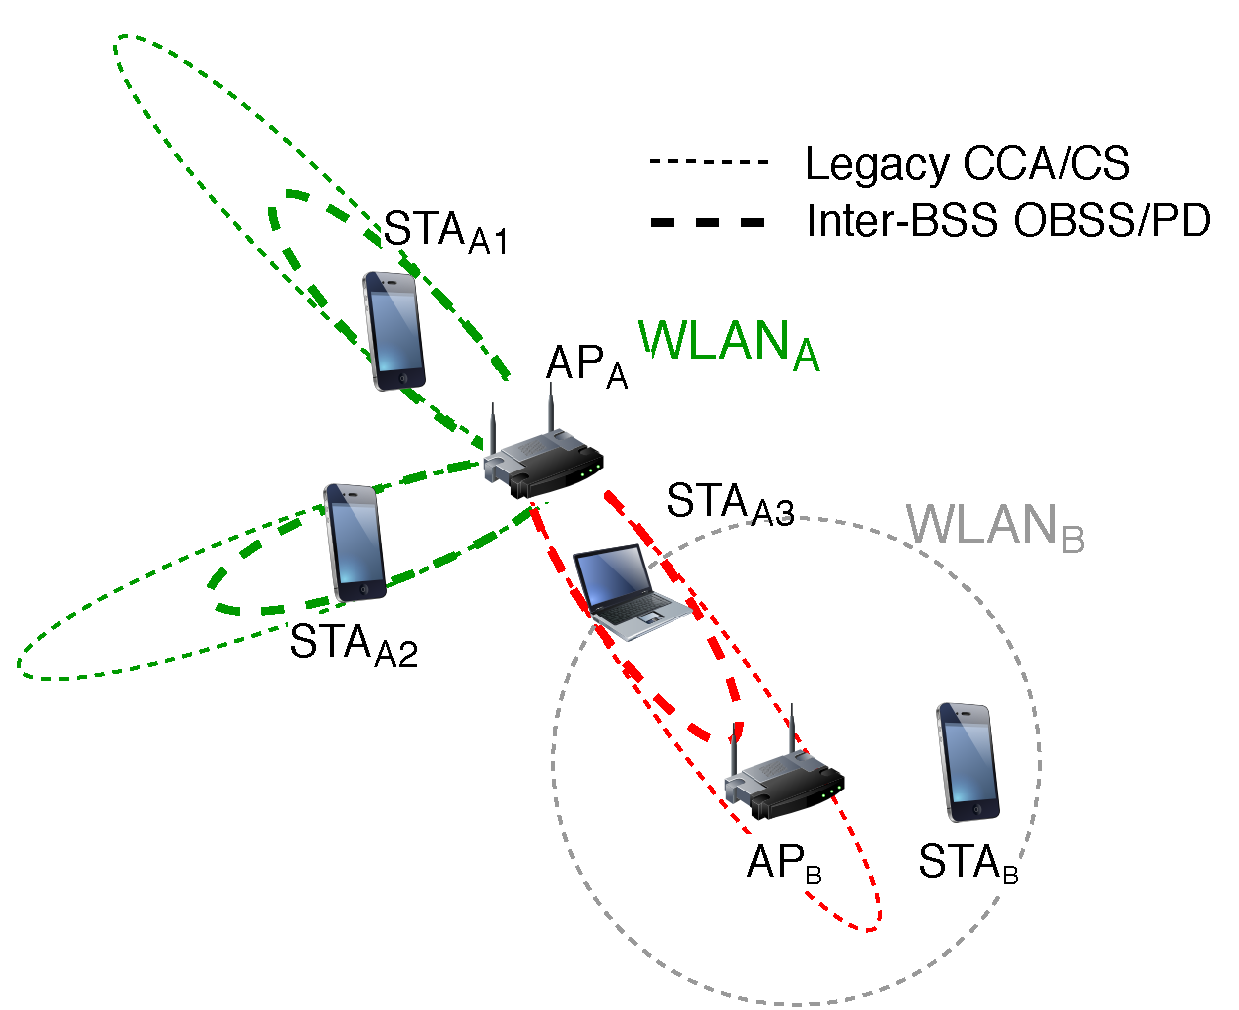
\includegraphics[width=0.9\columnwidth]{sr_and_beamforming}
		\caption{Potential application of SR combined with directional transmissions.}
		\label{fig:sr_and_beamforming}
	\end{figure}
	
	Similarly to the integration with directional antennas, the potential of SR can be further exploited through TB communications. In this case, users of a given WLAN can be categorized into different types, according to different inter-BSS OBSS/PD values to be used on them. Fig. \ref{fig:sr_and_tb_a} shows how users can be grouped based on different OBSS/PD thresholds. As a result, transmissions within the same WLAN can be scheduled in a different manner, thus increasing network efficiency. In our proposed example, $\text{STA}_\text{A1}$ and $\text{STA}_\text{A2}$ belong to the first group because of their privileged position with respect to $\text{AP}_A$. Therefore, a more aggressive OBSS/PD threshold is employed at the time of scheduling transmissions to these stations. The same logic can be applied to $\text{STA}_\text{A3}$, which, in this case, requires the usage of a more conservative OBSS/PD threshold for being scheduled in combination with SR. Finally, the legacy CCA/CS is used for $\text{STA}_\text{A4}$, in order to prevent negative interactions with respect to $\text{WLAN}_B$. It is worth pointing out that users belonging to different groups can be scheduled together, provided that the most restrictive PD threshold is used. 
	
	In Fig. \ref{fig:sr_and_tb_b}, we show a data transmission based on the combination of TB communications and SR. In the yellow point \#1, $\text{AP}_A$ detects an inter-BSS transmission from $\text{AP}_B$, which can be ignored by using the most aggressive OBSS/PD, i.e., the one devoted for STAs in group 1. Accordingly, it schedules an uplink transmission from $\text{STA}_\text{A1}$ and $\text{STA}_\text{A2}$ (yellow point \#2). Finally, $\text{AP}_A$ receives the scheduled transmissions from group 1 (yellow point \#3).
	
	\begin{figure}[ht!]
		\centering		
		\subfigure[Scenario]{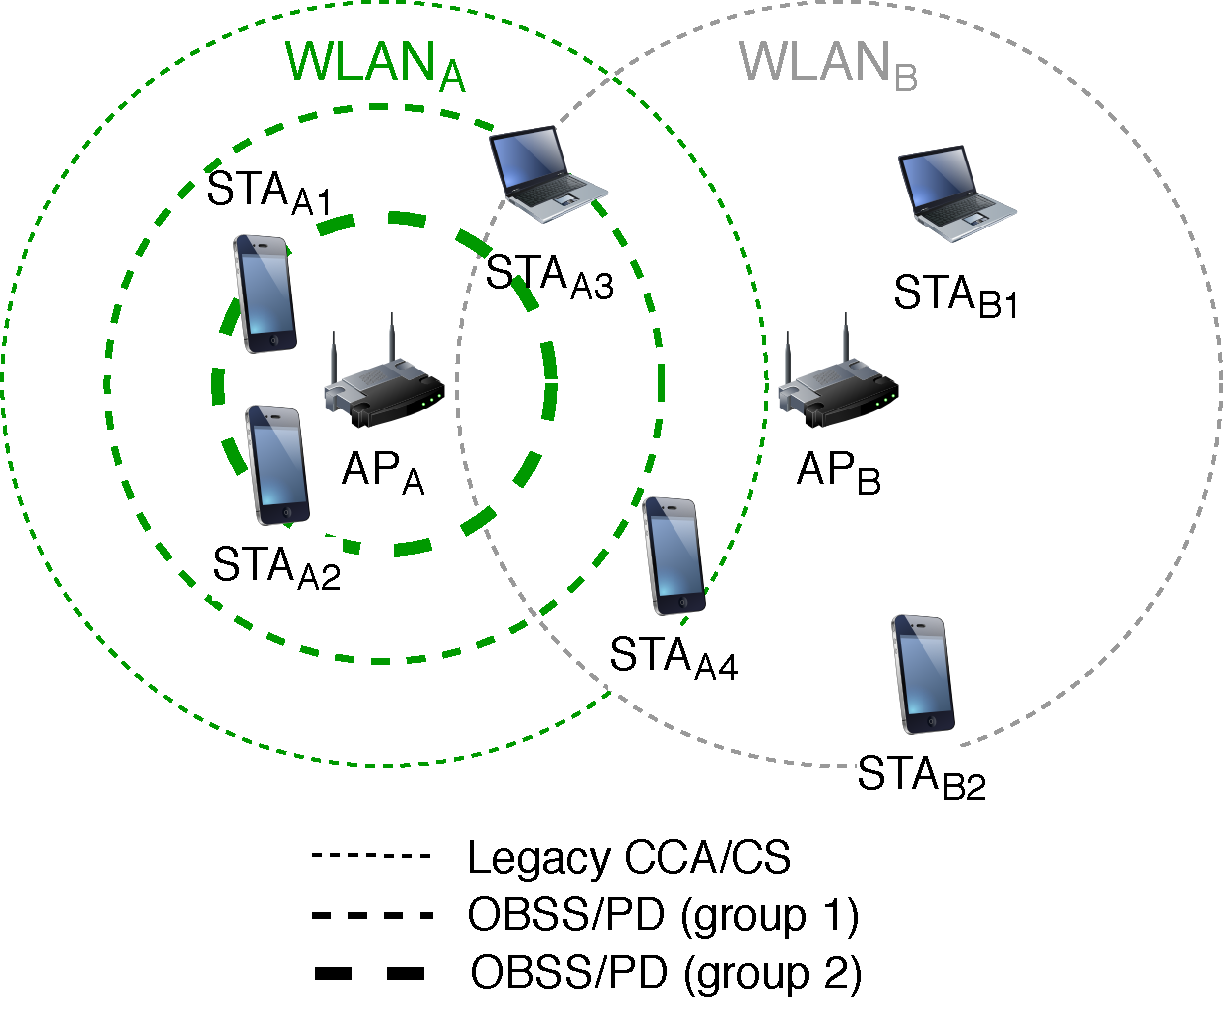
\includegraphics[width=0.8\columnwidth]{sr_and_tb}\label{fig:sr_and_tb_a}}
		\subfigure[Packets exchange]{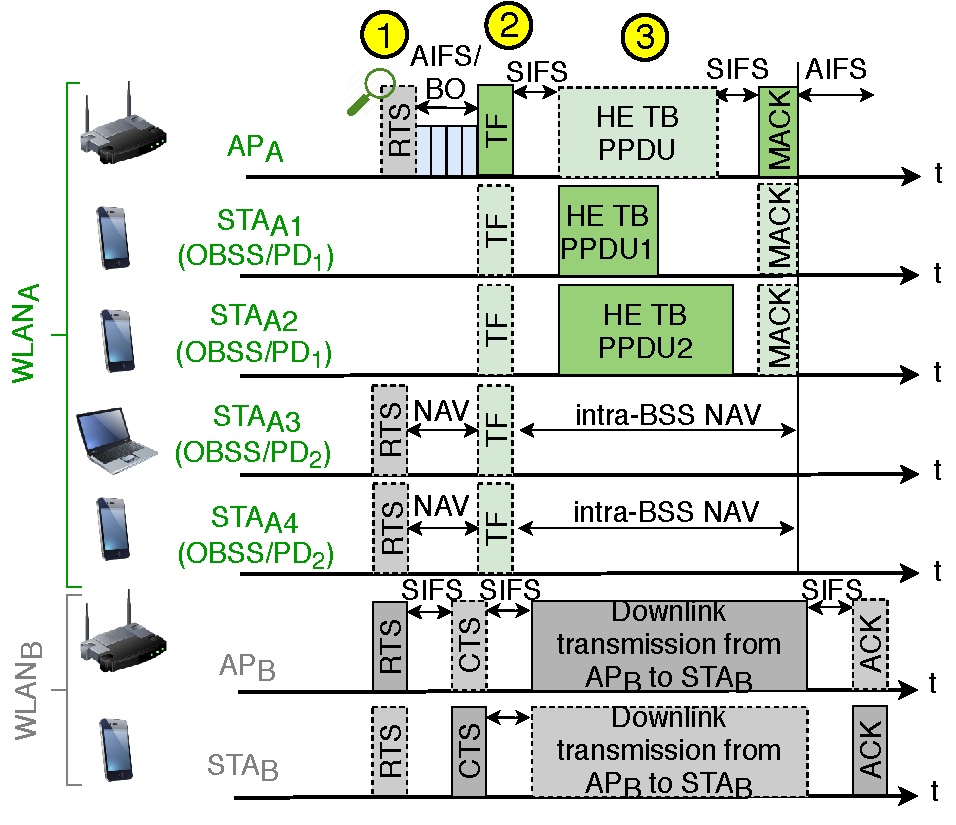
\includegraphics[width=\columnwidth]{sr_and_tb_b}\label{fig:sr_and_tb_b}}
		\caption{Potential application of SR combined with TB communications.}		\label{fig:sr_and_tb}
	\end{figure}
	
	\subsection{Artificial Intelligence to Address Spatial Reuse Optimization}
	
	In light of the challenges posed by the 11ax SR operation, Artificial Intelligence (AI) emerges as a potential solution. In particular, WLANs are characterized by being highly varying in terms of users and channel dynamics. Moreover, we typically find decentralized deployments, at which none or little coordination is allowed. Hence, online learning stands as a suitable technique to address the optimization of SR in WLANs. In fact, many works on PD adjustment, such as DSC \cite{smith2015dynamic} and COST \cite{selinis2018control}, are based on iterative methods. 
	
	Machine Learning (ML), and more precisely Reinforcement Learning (RL), can contribute to improving the performance of the already existing methods. RL has been shown to properly fit with the decentralized nature of IEEE 802.11 WLANs \cite{wilhelmi2019collaborative, wilhelmi2019potential}. In particular, the usage of RL allows capturing subtle information that cannot be predicted on before-hand (for instance, regarding inter-WLANs interactions). Such information enables conducting a proper learning procedure, which is aimed at increasing performance while reducing the number of undesired situations (e.g., poor fairness).
	
	% ----------------------------------
	% -
	% 	-- Conclusions --
	% -
	% ----------------------------------
	\section{Conclusions}
	\label{section:conclusions}
	
	In this paper, we have provided an extensive tutorial of the IEEE 802.11ax SR operation, which is aimed at maximizing the performance of next-generation WLANs by increasing the number of parallel transmissions. Our purpose has been to do so in a clear and easy-to-understand manner. Thus, significant efforts have been made in providing meaningful examples of the different specifications related to SR. %First of all, we have presented the concepts that enable such an operation, which mostly refer to BSS coloring, SRGs, and scheduled transmissions. From there, we described the 11ax SR specification, which has been supported with illustrative examples. 
	
	Apart from the tutorial, we have modeled the SR operation analytically using CTMNs. Through this model, we have analyzed the new kind of inter-WLAN interactions that may result from applying SR in an OBSS. In particular, we have considered WLANs with a single STA, but more complex interactions are expected to happen when applying the SR operation in WLANs with multiple STAs. In addition to the model, we have implemented the 11ax SR operation in the Komondor simulator. The potential of SR in large-scale scenarios has been evaluated through extensive simulations.
	
	Besides significant improvements are achieved through the SR operation, other important aspects are identified. First of all, it is important to highlight the non-intrusive characteristic of the SR operation. In particular, WLANs using this operation can increase their performance without affecting other overlapping networks or preventing them to transmit. This is a key feature for sustainable performance growth. Moreover, the SR operation has been shown to perform better in scenarios with a high level of interference, i.e., high-density scenarios with a high traffic load. This confirms the utility of the SR for dense next-generation wireless networks. 
	
	However, finding the best SR configuration is far from trivial (it is a combinatorial problem), and still remains open to the date. Indeed, the 11ax amendment does not provide any specification and/or guideline on this matter. We left as future work the design of mechanisms able to find the optimal parameters within the IEEE 802.11ax SR operation. For that purpose, the usage of RL will be particularly targeted. In addition, SR can be further enhanced by combining the operation with other novel techniques such as directional transmissions or distributed OFDMA.

	%%% APPENDICES
	\appendices
	\section{IEEE 802.11ax Frames}
	\label{section:frames}
	In this Section, we introduce the type of frames that are considered in the 11ax amendment. Such information is key to properly understand the SR operation.
	
	% HE PPDUs
	\subsection{HE PPDU formats}
	Below, we briefly describe the Physical Protocol Data Unit (PPDU) formats available in the 11ax:
	\begin{itemize}
		\item SU (Single User) HE PPDU: are meant for single user communications.
		\item  HE Extended Range HE PPDU: are meant for single user long-range transmissions, hence only contemplate 20 MHz bandwidths in a single spatial stream.
		\item  MU (Multi-User) HE PPDU: due to the OFDMA operation, such kind of PPDUs are meant for multiple transmissions to one or more users.
		\item Trigger-Based (TB) HE PPDU: in this case, MU UL transmissions are scheduled by the AP, which decides which STAs are expected to transmit during a specific elapse of time. The TB HE PPDUs can make use of OFDMA and/or MU-MIMO.
	\end{itemize}
	
	The new fields included in the abovementioned HE PPDU formats are HE Signal A Field (HE-SIG-A), HE Signal B Field (HE-SIG-B), HE Short Training Field (HE-STF), and HE Long Training Field (HE-LTF), which are shown in Fig. \ref{fig:appendix_1}.
	\begin{figure}[ht!]
		\centering
		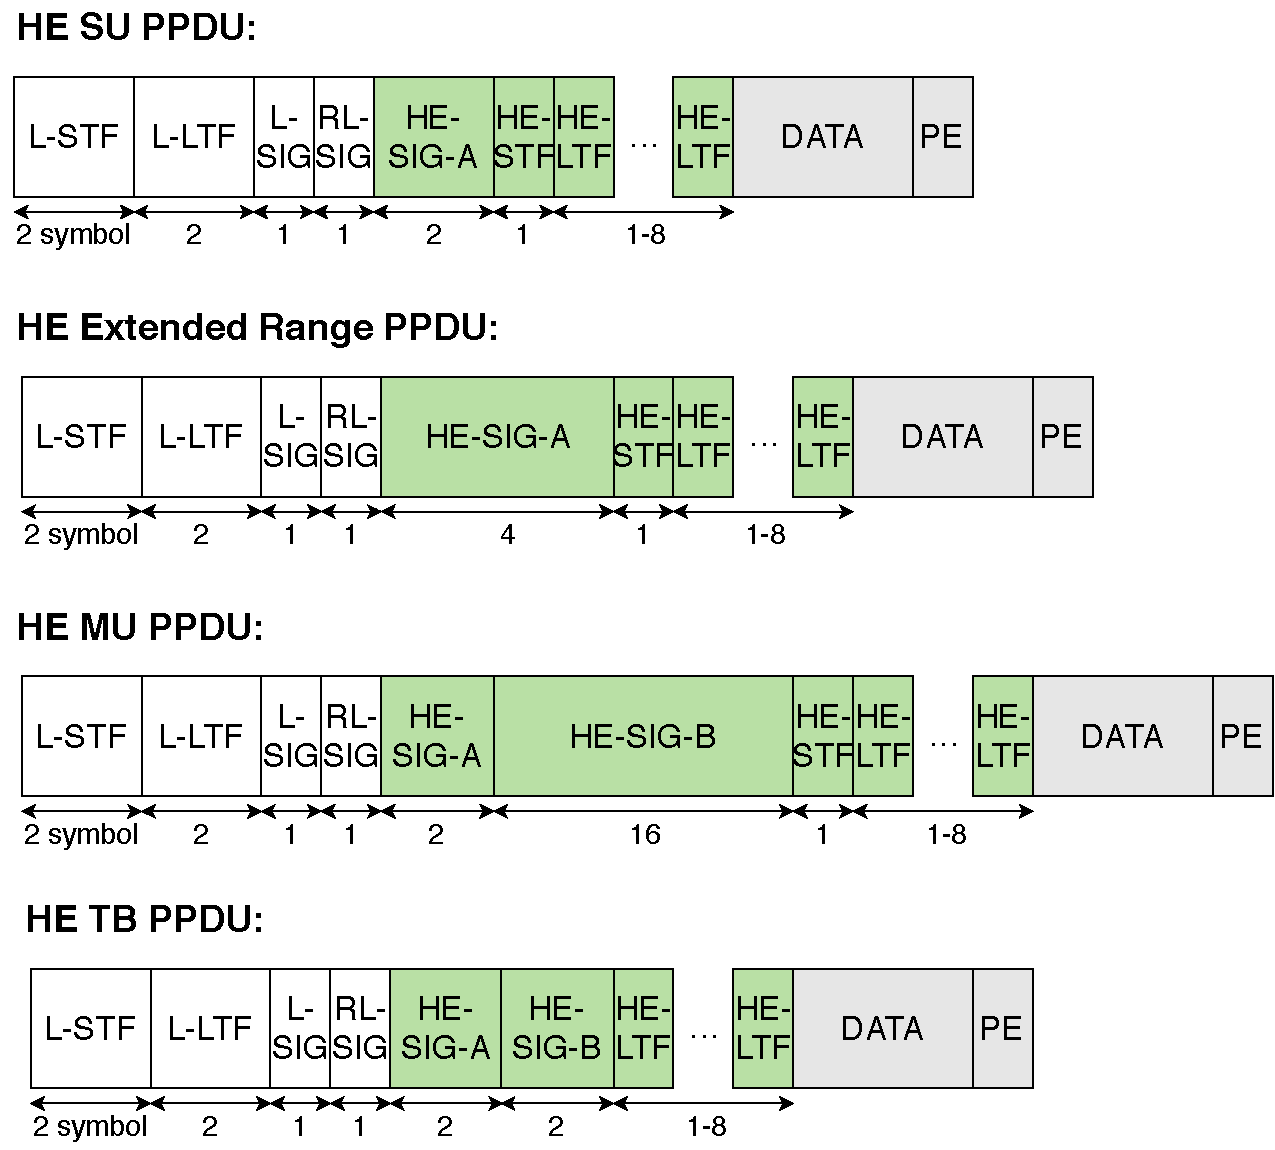
\epsfig{file=fig_25.pdf, width=\columnwidth}
		\caption{HE PPDU formats. New IEEE 802.11ax fields are highlighted in green.}
		\label{fig:appendix_1}
	\end{figure}
	
	Among the new fields, we highlight HE-SIG-A, which includes the following elements related to the SR operation:
		\begin{itemize}
			\item BSS color: it is used as an identifier of the BSS (refer to Section \ref{section:bss_coloring}).
			\item Spatial Reuse: this field indicates whether the HE node supports the SR operation. If this is the case, the field also indicates the limit on the transmission power to be used during the SR opportunities that can potentially be detected. Notice that a single Spatial Reuse field (of length of 4 bits) is carried in HE SU/MU/ER PPDUs,  while HE TB PPDUs may include up to four Spatial Reuse fields. In particular, each field is meant for the SR operation in each allowed channel width (i.e., 20 MHz, 40 MHz, 80 MHz, and 160 MHz).
	\end{itemize}
	
	Besides supporting HE PPDU formats, HE STAs are required to be compatible with legacy formats. More information regarding HE PPDU formats can be found in \cite{rhode2017whitepaper}. 
	
	% Other
	\subsection{Management Fields Implied in the Spatial Reuse Operation}
	Some operations auxiliary to SR are enabled by the exchange of control frames, which are Beacon, Probe Response, and (Re)Association Response frames. Beacons are a type of frame used by APs to announce the presence of a WLAN and to provide details of it. In particular, an AP, by means of Beacons, may request a STA to gather information regarding the environment: information of BSSs matching a particular BSSID and/or SSID, channel-specific report, or HE Operation element of neighboring HE APs. With such information, the AP can make decisions related to the SR operation. Regarding Probe Responses, they are meant to carry the information requested by devices scanning the area through Probe Requests. Finally, (Re)Association Response frames are sent by APs to which a station (STA) attempts to associate.
	
	The abovementioned kind of frames are important to the SR operation because they carry, among other fields, the following information:
	\begin{itemize}
		\item \textbf{HE Capabilities:} it is used by HE STAs to announce support for certain HE capabilities.
		\item \textbf{HE Operation:} it defines the operation of HE STAs. For instance, it indicates whether BSS coloring is enabled or not.
		\item \textbf{BSS Color Change Announcement:} it is used by HE APs to indicate the utilization of a new BSS color so that the associated STAs and the surrounding devices can be aware of the change.
		\item \textbf{Spatial Reuse Parameter Set (SRPS) element:} this element provides the necessary information to carry out the OBSS/PD-based SR operation, which is defined in Section \ref{section:obss_pd_based}. The SRPS element is further defined in Appendix \ref{section:srps}.
	\end{itemize}
	
	\subsubsection{Spatial Reuse Parameter Set element}
	\label{section:srps}
	The format of the SRPS element is optionally present in Beacons, Probe Responses and (Re)Association responses. Fig. 
	\ref{fig:appendix_2} shows the SRPS element in detail.
	% SR PARAMETER SET ELEMENT
	\begin{figure}[ht!]
		\centering
		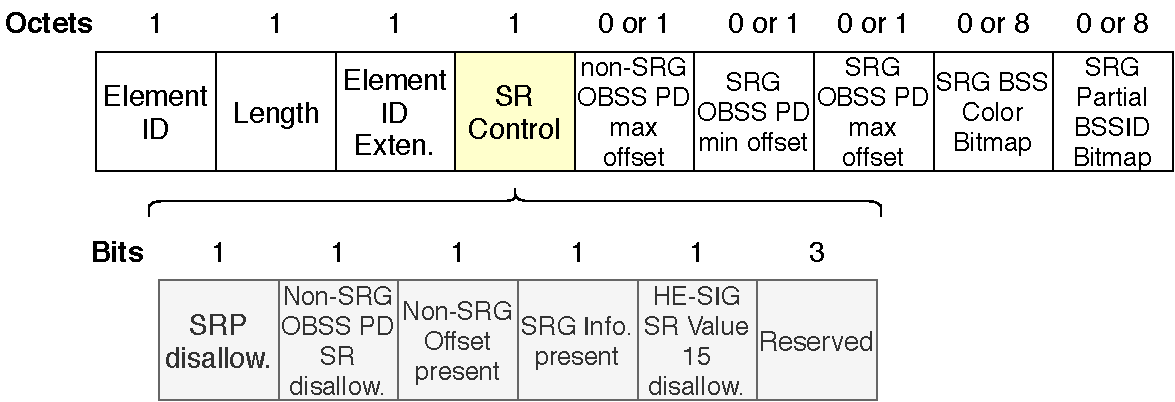
\epsfig{file=fig_26.pdf, width=\columnwidth}
		\caption{Spatial Reuse Parameter Set element.}
		\label{fig:appendix_2}
	\end{figure}
	
	Each item in the SRPS element is next described:
	\begin{itemize}
		\item Element ID: set to 255.
		\item Length: not defined.
		\item Element ID extension: set to 39.
		\item SR Control field: contains the following parameters:
		\begin{itemize}
			\item SRP Disallowed: indicates whether SRP-based SR transmissions are allowed or not at non-AP STAs that are associated with the AP that transmitted this element.
			\item Non-SRG OBSS/PD SR Disallowed: indicates whether non-SRG OBSS/PD SR transmissions are allowed or not at non-AP STAs that are associated with the AP that transmitted this element.
			\item Non-SRG Offset Present: indicates whether the Non-SRG OBSS/PD Max Offset subfield is present in the element.
			\item SRG Information Present: indicates whether the SRG OBSS/PD Min Offset, SRG OBSS/PD Max Offset, SRG BSS Color Bitmap, and SRG Partial BSSID Bitmap subfields are present in the element.
			\item HE-SIG-A Spatial Reuse Value 15 disallow: indicates whether non-AP STAs that are associated with the AP that transmitted this element may set the TXVECTOR parameter SPATIAL\_REUSE to SRP\_AND\_NON-SRG-OBSS-PD\_PROHIBITED to avoid SRP-based SR transmissions.
		\end{itemize}
		\item Non-SRG OBSS/PD Max Offset: integer to generate the maximum Non-SRG OBSS/PD threshold.
		\item Non-SRG OBSS/PD Min Offset: integer to generate the minimum Non-SRG OBSS/PD threshold.
		\item SRG OBSS/PD Max Offset: integer to generate the maximum SRG OBSS/PD threshold.
		\item SRG BSS Color Bitmap: indicates which BSS Color values are used by the members of the SRG.
		\item SRG Partial BSSID Bitmap: indicates which partial BSSID values are used by members of the SRG.
	\end{itemize}
	
	\section*{Acknowledgments}
	
	This  work  has  been  partially  supported  by  the  Spanish Ministry of Economy and Competitiveness under the Maria de Maeztu  Units  of  Excellence  Programme  (MDM-2015-0502), by PGC2018-099959-B-100 (MCIU/AEI/FEDER,UE), by the Catalan Government under SGR grant for research support (2017-SGR-11888), by SPOTS project (RTI2018-095438-A-I00) funded by the Spanish Ministry of Science, Innovation and Universities, and  by a Gift from the Cisco University Research Program (CG\#890107, Towards Deterministic Channel Access in High-Density WLANs) Fund, a corporate advised fund of Silicon Valley Community Foundation.
	
	% Can use something like this to put references on a page
	% by themselves when using endfloat and the captionsoff option.
	\ifCLASSOPTIONcaptionsoff
	\newpage
	\fi
	
	% trigger a \newpage just before the given reference
	% number - used to balance the columns on the last page
	% adjust value as needed - may need to be readjusted if
	% the document is modified later
	%\IEEEtriggeratref{8}
	% The "triggered" command can be changed if desired:
	%\IEEEtriggercmd{\enlargethispage{-5in}}
	
	% references section
	
	% can use a bibliography generated by BibTeX as a .bbl file
	% BibTeX documentation can be easily obtained at:
	% http://mirror.ctan.org/biblio/bibtex/contrib/doc/
	% The IEEEtran BibTeX style support page is at:
	% http://www.michaelshell.org/tex/ieeetran/bibtex/
	%\bibliographystyle{IEEEtran}
	% argument is your BibTeX string definitions and bibliography database(s)
	%\bibliography{IEEEabrv,../bib/paper}
	%
	% <OR> manually copy in the resultant .bbl file
	% set second argument of \begin to the number of references
	% (used to reserve space for the reference number labels box)
	%\begin{thebibliography}{1}
	%
	%\bibitem{IEEEhowto:kopka}
	%H.~Kopka and P.~W. Daly, \emph{A Guide to \LaTeX}, 3rd~ed.\hskip 1em plus
	%  0.5em minus 0.4em\relax Harlow, England: Addison-Wesley, 1999.
	%
	%\end{thebibliography}
	
	% -------------------------------------
	% Bibliography
	%
	% -------------------------------------
	\bibliographystyle{unsrt}
	\bibliography{bib}
	
	% biography section
	% 
	% If you have an EPS/PDF photo (graphicx package needed) extra braces are
	% needed around the contents of the optional argument to biography to prevent
	% the LaTeX parser from getting confused when it sees the complicated
	% \includegraphics command within an optional argument. (You could create
	% your own custom macro containing the \includegraphics command to make things
	% simpler here.)
	%\begin{IEEEbiography}[{\includegraphics[width=1in,height=1.25in,clip,keepaspectratio]{mshell}}]{Michael Shell}
	% or if you just want to reserve a space for a photo:
	
	\begin{IEEEbiography}[{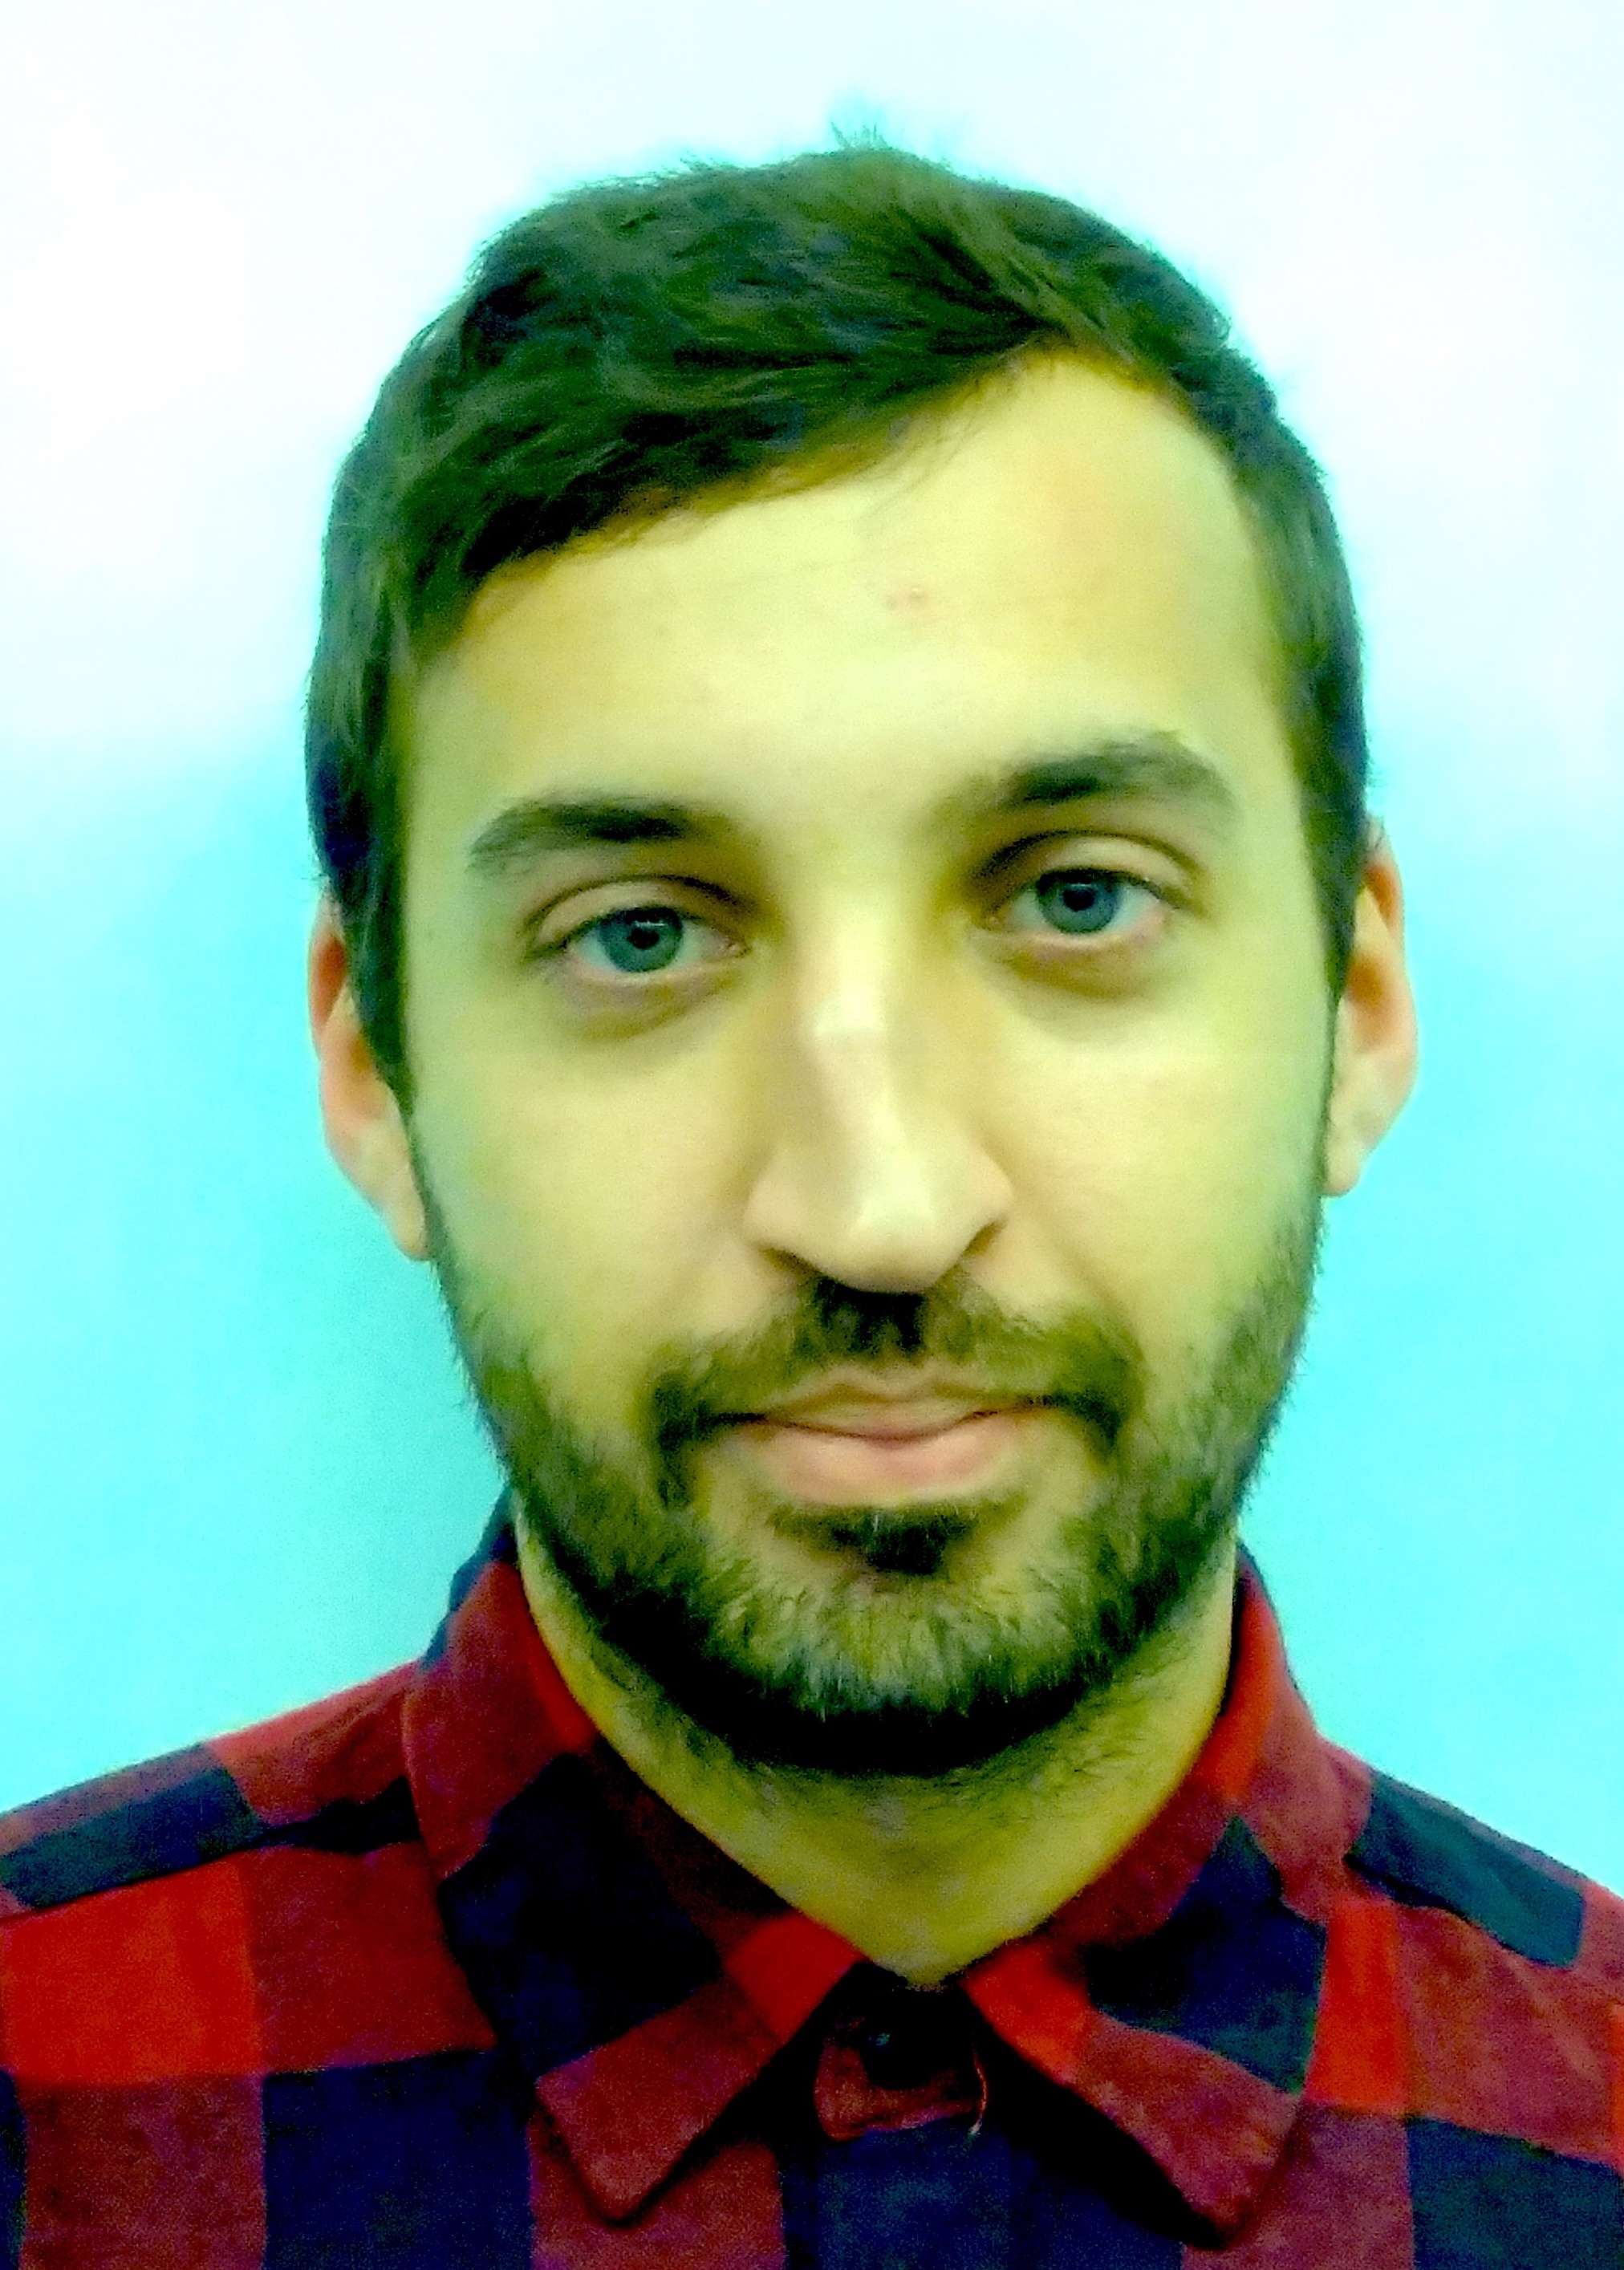
\includegraphics[width=1in,height=1.25in,clip,keepaspectratio]{fwilhelmi}}]{Francesc Wilhelmi} holds a B.Sc. degree in Telematics Engineering (2015) and a M.Sc. in Intelligent and Interactive Systems in (2016), both from Universitat Pompeu Fabra (UPF). He is currently a Ph.D. Student in the Wireless Networking Research Group (WNRG) in the Department of Information and Communication Technologies (DTIC) at the UPF. His interests are related to next-generation wireless networks and their potential synergy with Artificial Intelligence (AI).
	\end{IEEEbiography}
	
	\begin{IEEEbiography}[{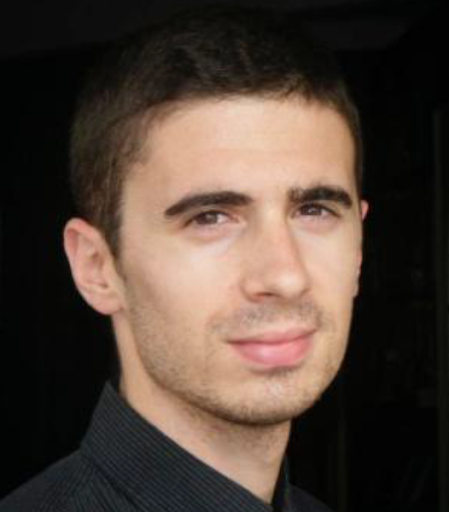
\includegraphics[width=1in,height=1.25in,clip,keepaspectratio]{sbarrachina}}]{Sergio Barrachina-Mu\~noz} obtained his B.Sc. degree in Telematics Engineering and his M.Sc. in Intelligent Interactive Systems in 2015 and 2016, respectively, both from Universitat Pompeu Fabra (UPF), Barcelona. Currently, he is a PhD student and teacher assistant in the Department of Information and Communication Technologies (DTIC) at UPF. His main research interests are focused on developing autonomous learning methods and techniques for improving the performance of next-generation wireless networks.
	\end{IEEEbiography}
	
	\begin{IEEEbiography}[{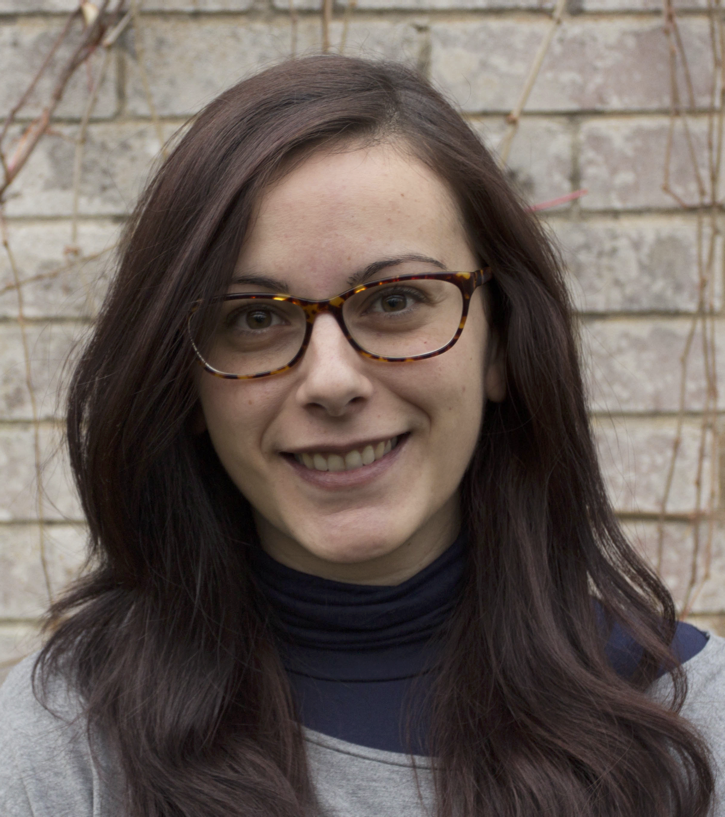
\includegraphics[width=1in,height=1.25in,clip,keepaspectratio]{cristina2}}]{Cristina Cano} holds a Ph.D. (2011) in Information, Communication and Audiovisual Media Technologies from the Universitat Pompeu Fabra (UPF). She has been a research fellow in the Hamilton Institute of the National University of Ireland, Maynooth (2012-2014), in Trinity College Dublin (2015-2016) and in Inria- Lille in France (first half of 2016). Currently, she is an associate professor at the WINE research group of the Universitat Oberta de Catalunya (UOC). Her research interests include coexistence of wireless heterogeneous networks, distributed resource allocation and online optimisation. 
	\end{IEEEbiography}
	
	\begin{IEEEbiography}[{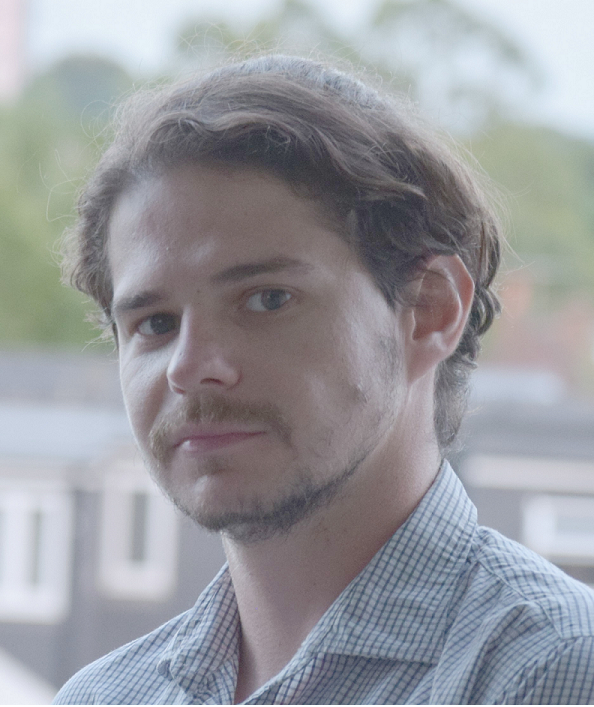
\includegraphics[width=1in,height=1.25in,clip,keepaspectratio]{selinis_pic}}]{Ioannis Selinis} received the B.Sc. and M.Sc. degrees from University of Piraeus, Greece, in 2011 and 2014, respectively. He is currently a research fellow and pursuing a Ph.D in electronic engineering from the Institute for Communications Systems (ICS) home of the 5G Innovation Centre at the University of Surrey. His main research interests include wireless communications and networking, performance evaluation and design of MAC protocols.
	\end{IEEEbiography}

	\begin{IEEEbiography}[{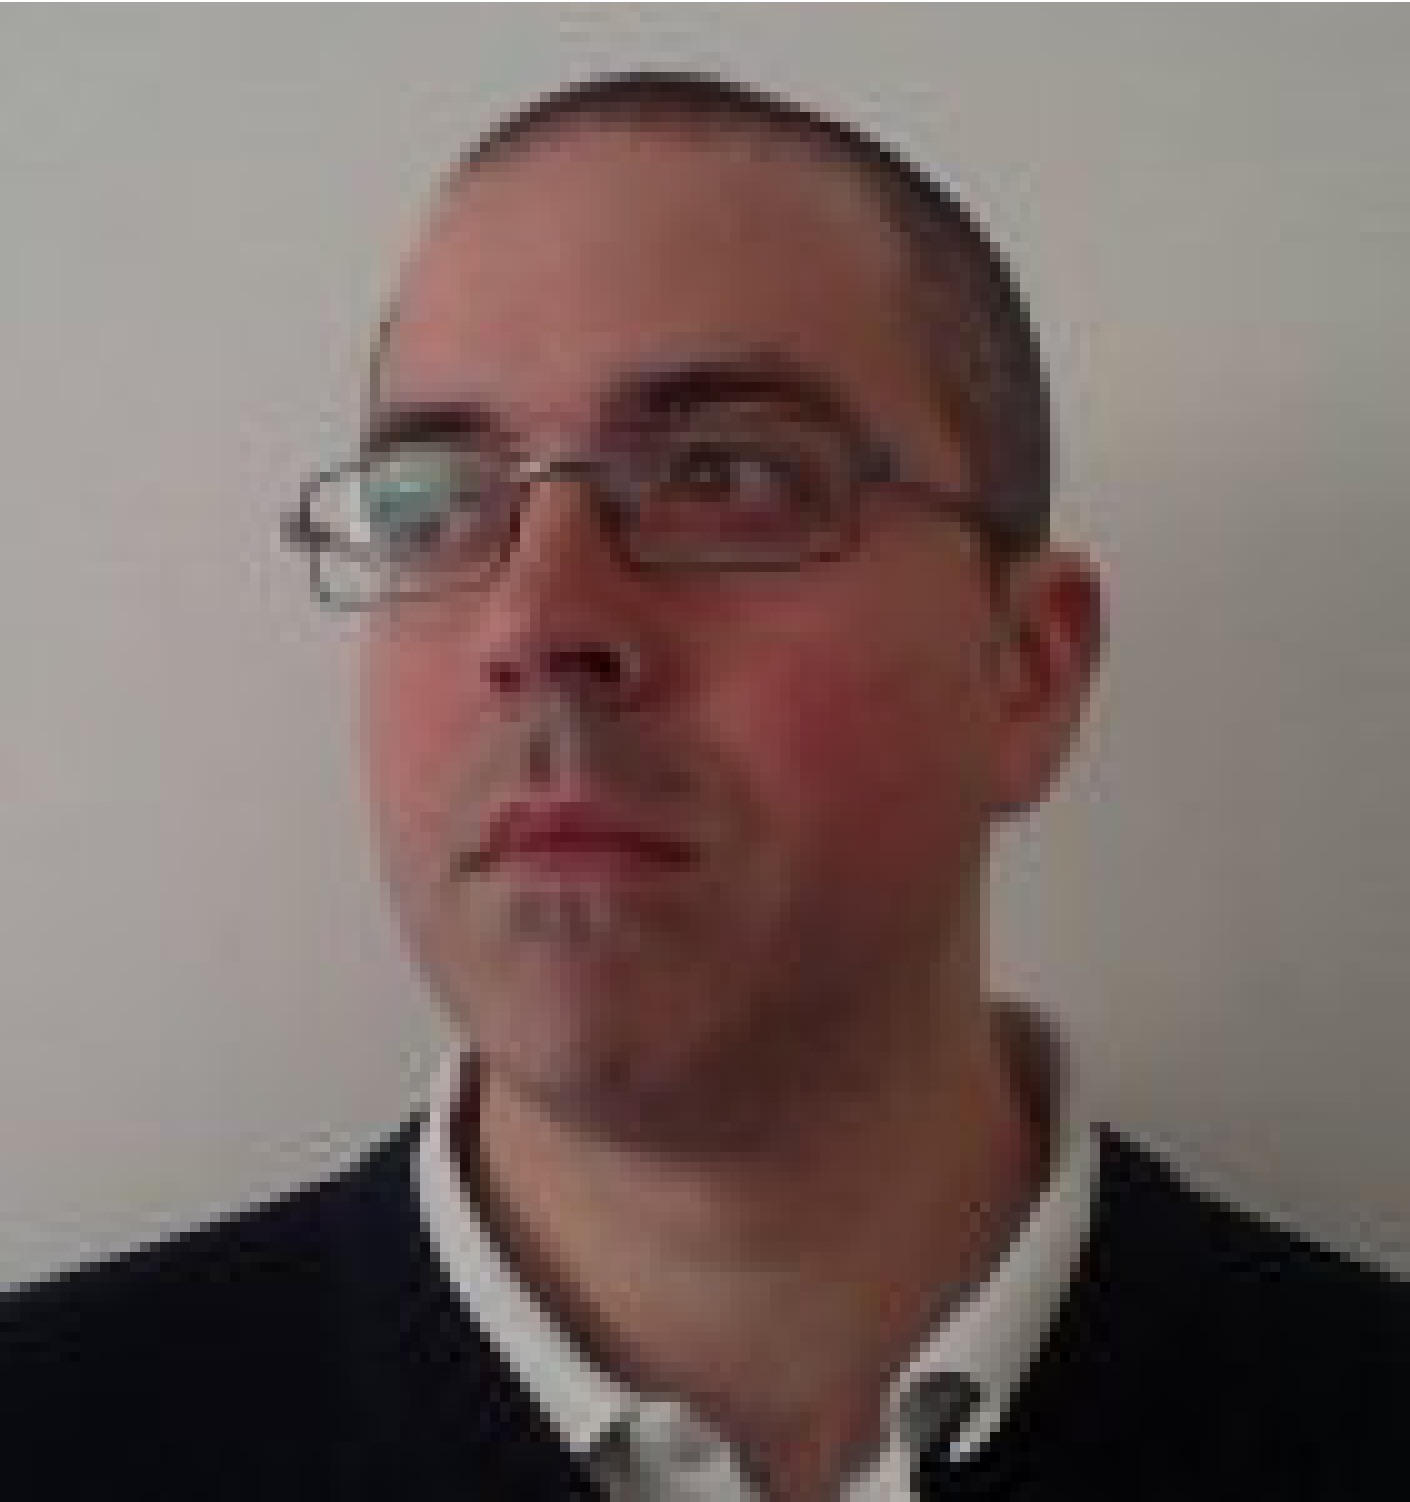
\includegraphics[width=1in,height=1.25in,clip,keepaspectratio]{bbellalta}}]{Boris Bellalta} is an Associate Professor in the Department of Information and Communication Technologies (DTIC) at Universitat Pompeu Fabra (UPF). He is the head of the Wireless Networking research group at DTIC/UPF. His research interests are in the area of wireless networks, with emphasis on the design and performance evaluation of new architectures and protocols.
	\end{IEEEbiography}

	% You can push biographies down or up by placing
	% a \vfill before or after them. The appropriate
	% use of \vfill depends on what kind of text is
	% on the last page and whether or not the columns
	% are being equalized.
	
	%\vfill
	
	% Can be used to pull up biographies so that the bottom of the last one
	% is flush with the other column.
	%\enlargethispage{-5in}
	
	% that's all folks
\end{document}